% !TEX encoding = UTF-8 Unicode
% !TEX root = DesignDocument.tex

\documentclass{book}

% !TEX root = DesignDocument.tex



\usepackage[width=6.5in, height=9.2in, top=1.0in, papersize={8.5in,11in}]{geometry}
\usepackage[pdftex]{graphicx}
\graphicspath{{Graphics/}}
\usepackage{amsmath}
\usepackage{amsthm}
\usepackage{amssymb}
%\usepackage{txfonts}
\usepackage{textcomp}
\usepackage{amsthm}
\usepackage{float}
\usepackage[all]{xy}
\usepackage{fancyhdr}
\pagestyle{fancy}
\usepackage{hyperref}
\usepackage{verbatim}
\usepackage{algorithm}
\usepackage{algorithmic}
\usepackage{array}
\usepackage{color}
\usepackage{listings}
\usepackage{calc}
\usepackage{doxygen}
\usepackage[utf8]{inputenc}
\usepackage{makeidx}
\usepackage{multicol}
\usepackage{multirow}
\usepackage[table]{xcolor}
\usepackage{tabularx}
\usepackage{framed}
\usepackage{xspace}
\usepackage{etex}
\usepackage{todonotes}
\usepackage{pdfpages}
\usepackage{pgfgantt}


%% Computer Modern Bright Font
%\usepackage{cmbright}
%\usepackage[T1]{fontenc}

%% Sans Serif Modern Font - similar to  Helvetica
\usepackage{lmodern}
\renewcommand*\familydefault{\sfdefault} %% Only if the base font of the document is to be sans serif
\usepackage[T1]{fontenc}


\definecolor{SDColor1}{rgb}{0,0,0}
\definecolor{SDColor2}{rgb}{0,0,0}
\definecolor{SDColor3}{rgb}{0,0,0}
\definecolor{SDColor4}{rgb}{0,0,0}
\definecolor{SDColor5}{rgb}{0,0,0}

%%%  --- Here are some other colors.  Keep it conservative --- %%%

%% Blue font color scheme
%\definecolor{SDColor1}{rgb}{.204,.353,.541}
%\definecolor{SDColor2}{rgb}{.31,.506,.741}
%\definecolor{SDColor3}{rgb}{0.18,0.35,0.59}
%\definecolor{SDColor4}{rgb}{0.44,0.59,0.82}
%\definecolor{SDColor5}{rgb}{0.35,0.35,0.35}
%

% Brown color scheme
% \definecolor{SDColor1}{rgb}{.55,.2,.2}
%\definecolor{SDColor2}{rgb}{.4,.1,.1}
%\definecolor{SDColor3}{rgb}{.5, .15,.15}
%\definecolor{SDColor4}{rgb}{.63,.32,.18}
%\definecolor{SDColor5}{rgb}{.45,.15,.15}
%


%% Custom colors for code listing environment
\definecolor{OliveGreen}{cmyk}{0.64,0,0.95,0.40}
\definecolor{DarkBlue}{cmyk}{0.76,0.76,0,0.20}
\definecolor{DarkRed}{cmyk}{0,1,1,0.45}
\lstset{language=c,frame=ltrb,framesep=5pt,basicstyle=\normalsize,
 keywordstyle=\ttfamily\color{DarkRed},
identifierstyle=\ttfamily\color{DarkBlue}\bfseries,
commentstyle=\color{OliveGreen},
stringstyle=\ttfamily,
showstringspaces=false,tabsize = 3}


\setlength{\oddsidemargin}{0mm} 
\setlength{\evensidemargin}{0mm} 

%% Uncomment if you want "Draft" placed on each page.
%\usepackage{draftwatermark}
%\SetWatermarkLightness{0.975}
%\SetWatermarkScale{1}
%\SetWatermarkText{Draft}

\pagestyle{fancy}
\renewcommand{\chaptermark}[1]{\markboth{#1}{}}
\renewcommand{\sectionmark}[1]{\markright{\thesection\ #1}}
\fancyhf{}
\fancyhead[LE,RO]{\bfseries\thepage}
\fancyhead[LO]{\bfseries\rightmark}
\fancyhead[RE]{\bfseries\leftmark}
%\fancyfoot[LE,RO]{Confidential and Proprietary}
%\renewcommand{\headrulewidth}{0.5pt}
%\renewcommand{\footrulewidth}{0pt}
%\addtolength{\headheight}{0.5pt}
%\setlength{\footskip}{0mm}
%\renewcommand{\footruleskip}{0pt}



\usepackage{titlesec}
\titleformat{\chapter}[display]
{\normalfont\bfseries\color{SDColor3}}    %\normalfont\bfseries\filcenter}
{\LARGE\thechapter}
{1ex}
{\titlerule[2pt]
\vspace{2ex}%
\LARGE}
[\vspace{1ex}%
{\titlerule[2pt]}]

%
%\usepackage{titlesec}
%\titleformat{\chapter}{\normalfont\bfseries\LARGE}
%{\thechapter.}{5pt}{}[{\titlerule[3pt]}]
%
%\titleformat{\section}{\normalfont\bfseries\Large}
%{\thesection.}{5pt}{}[{\titlerule[2pt]}]
%
%\titleformat{\subsection}{\normalfont\bfseries\large}
%{\thesubsection.}{5pt}{}[{\titlerule[1pt]}]
%


%\titleformat*{\section}{\Large\bfseries\sffamily\color{SDColor1}}
%\titleformat*{\subsection}{\large\bfseries\sffamily\color{MSLightBlue}}
%\titleformat*{\section}{\Large\bfseries\color{SDColor3}}
%\titleformat*{\subsection}{\large\bfseries\color{SDColor4}}

%\titleformat*{\section}{\Large\bfseries}
%\titleformat*{\subsection}{\large\bfseries}
%\titleformat*{\subsubsection}{\large\bfseries}

\titleformat*{\section}{\Large\bfseries\color{SDColor1}}  
\titleformat*{\subsection}{\large\bfseries\color{SDColor2}}
\titleformat*{\subsubsection}{\large\bfseries\color{SDColor5}}
\setcounter{secnumdepth}{3}
\renewcommand{\thesubsubsection}{\thesubsection.\alph{subsubsection}}

% Save the original chapter command as stdchapter
\let\stdchapter\chapter

%redefine the backmatter command
\let\stdbackmatter\backmatter
\makeatletter% We need the '@' letter to call if@openright
\renewcommand{\backmatter}{
\stdbackmatter
% need to set the page counter back to 1
\setcounter{page}{1}
%% Redefine the \chapter command for our Back Matter
\renewcommand{\chapter}[1]{
  \if@openright\cleardoublepage\else\clearpage\fi% chapters begin on right page
  \stdchapter{##1}% output standard chapter heading
  \setcounter{section}{0}% restart the section numbering
  \renewcommand{\thepage}{BM-\arabic{page}}% Redefine page numbering format
  \renewcommand{\thesection}{\arabic{section}}% Redefine section number format
}}
\makeatother% Restore the normal behavior of '@'

%redefine the appendix command
\let\stdappendix\appendix
\makeatletter% We need the '@' letter to call if@openright
\renewcommand{\appendix}{
\stdappendix
%% \titleformat{\chapter}[display]
%% {\normalfont\bfseries\color{SDColor3}}    %\normalfont\bfseries\filcenter}
%% {\LARGE Appendix \thechapter}
%% {1ex}
%% {\titlerule[2pt]
%% \vspace{2ex}%
%% \LARGE}
%% [\vspace{1ex}%
%% {\titlerule[2pt]}]
  %%% Since counters are different in the appendix section
  %%% we redefine \chapter to explicitly reset the page number
  %%%  (comment out to see effect)
  \renewcommand{\chapter}[1]{
    \stdchapter{##1}\setcounter{page}{1}
    %%% We also redefine page numbering
    \renewcommand{\thepage}{\Alph{chapter}-\arabic{page}}
  }
}
\makeatother% Restore the normal behavior of '@'


\makeatletter% We need the '@' letter to call if@openright
\newcommand{\agreement}{
  \renewcommand{\chapter}[1]{
    \if@openright\cleardoublepage\else\clearpage\fi% chapters begin on right page
    \pagestyle{plain}% turn off fancy headers
    \setcounter{section}{0}% Reset the section number
    \setcounter{page}{1}% Reset the page number
    \renewcommand{\thepage}{SA-\arabic{page}}% Set format for page numbering
    \renewcommand{\thesection}{\arabic{section}}% Set format for section numbering
    \refstepcounter{chapter}% Add it to the index/toc for on-line viewing
    \addcontentsline{toc}{chapter}{##1}% Add to the table of contents
  }
}
\makeatother% Restore the normal behavior of '@'



%%  If you do some math typesetting, you may want more environment names.
%% Uncomment to see how this works:
%\newtheorem{summary}{Summary:}
%\newtheorem{example}{Example:}



 % This sets the format.

% Add your title page contents here 
\newcommand{\teamName}{Augmented Education}
\title{{\color{SDColor3} \rule{\linewidth}{0.5mm}}\\[2mm] {\huge \bfseries \color{SDColor3} \teamName}\\[-1mm] {\color{SDColor3}\rule{\linewidth}{0.5mm}} \\  \vfill
{\LARGE \bfseries \color{SDColor4} Senior Design Final Documentation }\\  \vfill 
{\color{SDColor3} \teamName} }
\author
{
	\color{SDColor3} Aaron Alphonsus 
	\and \color{SDColor3} Cheldon Coughlen 
	\and \color{SDColor3} Daniel Hodgin 
	\and \color{SDColor3} Kenneth Petry 
	\and \color{SDColor3} Savoy Schuler
	\and \color{SDColor3} Brady Shimp
}

\date{\color{SDColor3} \today}


\begin{document}

\frontmatter

\addcontentsline{toc}{chapter}{Title}
\maketitle
\tableofcontents
\addcontentsline{toc}{chapter}{Contents}
\listoffigures
\addcontentsline{toc}{chapter}{List of Figures}
\listoftables
\addcontentsline{toc}{chapter}{List of Tables}
%\listofalgorithms
%\addcontentsline{toc}{chapter}{List of Algorithms}


\chapter{Document Preparation and Updates}
% !TEX root = DesignDocument.tex



Current Version [1.0.7]
\vspace*{5mm}

% I'll let everyone add their names individually here
{\color{SDColor5}
\noindent
\textit{Prepared By:}\\
\textit{Kenneth Petry}\\
\textit{Brady Shimp}\\
\textit{Savoy Schuler}\\
\textit{Cheldon Coughlen}\\
\textit{Daniel Hodgin}\\
\textit{Aaron Alphonsus}
}

\vfill
\noindent
{\color{SDColor3} \textit{\textbf{Revision History}}}\\
\begin{tabular}{|>{\raggedright}p{1.5cm}|>{\raggedright}p{3cm}|>{\raggedright}p{1.5cm}|>{\raggedright}p{9cm}|}
  \hline
  \textit{\textbf{Date}} &  \textit{\textbf{Author}} & \textit{\textbf{Version}} & \textit{\textbf{Comments}}\tabularnewline
  \hline
  \textit{\textbf{10/10/17}} & \textit{Kenneth Petry} & \textit{0.0.0} & \textit{Initial template}\tabularnewline\hline
  \textit{\textbf{12/04/17}} & \textit{Savoy Schuler} & \textit{1.0.0} & \textit{Added first half of project overview, high-level design, Software Agreement, Business Plan, Product Description, Acknowledgement.}\tabularnewline\hline
  \textit{\textbf{12/04/17}} & \textit{Brady Shimp} & \textit{1.0.0} & \textit{Added Sprint review and prototype documentation.}\tabularnewline\hline
  \textit{\textbf{12/04/17}} & \textit{Aaron Alphonsus} & \textit{1.0.0} & \textit{Added User stories requirements, product backlog, and Mobile Computing Grant}\tabularnewline\hline
  \textit{\textbf{12/04/17}} & \textit{Daniel Hodgin} & \textit{1.0.0} & \textit{Added Website design and class documentation, and toolchain description.}\tabularnewline\hline
  \textit{\textbf{12/04/17}} & \textit{Cheldon Coughlen} & \textit{1.0.0} & \textit{Added Test planning documentation.}\tabularnewline\hline
  &  &  & \tabularnewline
  \hline
  &  &  & \tabularnewline
  \hline
  &  &  & \tabularnewline
  \hline
  &  &  & \tabularnewline
  \hline
\end{tabular}
\vfill


 
 
 %%%   \chapter{Preface}  Uncomment if you want to have a preface ...
%%%  This is ..


\mainmatter

%% The term "cleaning" used in the syllabus means removing all of the sample content I
%% have provided.   You can comment out by using the comment character or the comment
%% environment.  

%%  Add to the following chapters

% !TEX root = DesignDocument.tex


\chapter{Overview, Description and Deliverables}

% The overview should take the form of an executive summary.  Give the reader a feel 
% for the purpose of the document, what is contained in the document, and an idea 
% of the purpose for the system or product. 

\section{Team Members and Team Name}

Team Name: Augmented Education

\noindent Team Members:
\begin{itemize}
	\item Aaron Alphonsus
	\item Cheldon Coughlen
	\item Daniel Hodgin
	\item Kenneth Petry
	\item Savoy Schuler
	\item Brady Shimp
\end{itemize}

\section{Client}
% A description of the client or customer.
% Description of sponsor if different than client.
% Brief statement of customer's problem or goal for this project
% List the customer needs

The project client is the South Dakota School of Mines and Technology (SD Mines) which will be purchasing a one-year Early Adopter License for the product. The client is intending to use the product to enhance the traditional education experience by integrating media unique to augmented reality in the classroom. The client needs a platform through which three-dimensional computer aided design files may be uploaded, cloud hosted, and delivered to an augmented reality device for rendering via a QR code associated with the uploaded file. The client will also need to be able to manage files and would like a collaboration space available for public and private sharing of files. 

The project sponsor is InTouch L.L.C., a custom software solutions provider specializing in mixed reality software. The sponsor needs the product to adequately meet the expectations set forth by its contract with the client. 

\section{Product}
% A high level description of the project.  Project environment ...
% Project boundaries.
% Project context.
% Technical Environment.
% Current systems overview.


\subsection{Description}
Augmented Education is a platform allowing three-dimensional models made with common computer-aided design (CAD) programs to be cloud hosted, converted, and made on-demand available to augmented reality viewing devices and mobile phones through download links such as QR codes that may be embedded in textbooks, presentations, and other media to enhance the traditional classroom experience. Once a 3D design has been accessed via QR code and rendered, the student may manipulate the rendering as supported by individual AR devices. 

\subsection{Product Vision}
Long term product evolution is visualized in the following phases. The product will be delivered to end users upon completion of the first phase. The licensing model will allow the following two phases to commence with user feedback and active revenue streams. 

\begin{itemize}
\item Phase One - current development - QR code and multi-platform visualization.
\item Phase Two - social platform to share models and collaboration both within universities and across other educational institutions.
\item Phase Three - full blown platform with API ecosystem that connects all sorts of data from various applications to visualize and collaborate.
\end{itemize}

\subsection{Phase One Features}
\begin{itemize}
	\item Users may use the website interface to upload files from a CAD program commonly used in STEM education. 
	\item  Upon upload files will be converted into a ubiquitous file format available for AR rendering. 
	\item The user will be returned a QR code that may be embedded in textbooks, homeworks handouts, PowerPoint presentations, emails, etc. 
	\item When an AR headset or mobile phone is used to view the QR code, the device will locate and render the associated file in augmented reality for the user.  
	\item Certain devices will allow the user motion control abilities to interact with the renderings so that they may be moved, scaled, rotated, animated, or “flipped through” in steps. 
	\item Cloud hosting will make the user’s files available anywhere at any time. 
	\item The web interface will allow for the management of files (add, delete, update, download). 
\end{itemize}

\subsection{Phase Two Features}
\begin{itemize}
	\item Web interface privacy settings will allow designs to be private, public, or accessible only by a “group” such as an institution. 
	\item A page will be added for showcasing popular public designs. 
	\item The public design page will have filtering abilities for sorting designs by upload date, most viewed, and by time periods. 
	\item Users will have a personal feed showcasing designs from collaboration groups. 
\end{itemize}

\subsection{Phase Three Features}
\begin{itemize}
	\item Expand platform to support broad range of file types for the purpose of increasing the number of CAD programs supported. 
	\item Expand platform to support broad range of hardware for the purpose of increasing number of AR devices supported. This may include adding support for output file types or application development for hardware. 
\end{itemize}


\subsection{Intellectual Property}
Patent application for elements of process pending. 

\subsection{Value} 
A/B testing targeting student engagement, retention, and conceptual clarity will be conducted in classrooms at the South Dakota School of Mines and Technology. Tests will be performed for several semesters wherein one section of a course taught by a given professor will be able to utilize our technology in the classroom as a learning aid and the other will not. 

The time required for an engineer to be trained in the transition between student and working professional averages in the range of 1-2 years. A result of the goal of enhancing the traditional educational experience with this service is to eliminate a large portion of the training required for students to make the transition to professionals in their fields. The test results will be able to support the claim that this service will reduce the amount of time is required to successfully make this transition.  With the average entry level engineering salary at about \$70,500, meaning up to \$141,000 or more in training expenses per entry level hire, Augmented Education aims to cut this need in half by providing students with a more immersive approach to learning and mastering concepts of design and structure. This is envisioned through noting that, should the new in-classroom experience create more effective learning, more topics and depth will be able to be taught per course. 

\subsection{Value Testimonials}
“Education is an industry based on entertainment. You can learn everything about Calculus from a 1960’s textbook. The information is the same today as it was then, but new textbooks are sold because they are printed in color and with better pictures. Students use Youtube tutorials to learn math because it is effective. The reason people pay for classes with instructors is because we balance presenting information with entertaining the student’s interest in it. Augment reality in education is that next step in creating a more engaging and entertaining learning environment.” - Dr. Jeff McGough, Computer Science and Mathematics Professor at SDSMT and founder of InTouch L.L.C.

“As an industrial engineering instructor, I run labs where students build bridges and motors using Lego bricks. I do it because it's interactive and helps communicate some of the early concepts. If I could  have system where students could instead see the components of these structures in an animated 3D environment that they could interact with, I would implement it immediately.” - Dr. Adam Piper, Industrial Engineer Professor at SDSMT



\subsection{Mission Statement}
InTouch L.L.C. pursues the mission of developing augmented reality and virtual reality (known together as “mixed reality”) solutions for education and enterprise. Hardware and entertainment software for this technology have matured over the past decade while innovators have, until now, overlooked the opportunity to leverage this same technology for applications such as classroom education, 3D advertising, architecture design, pre-construction modeling, and more.  

\subsection{Elevator Pitch}
Augmented reality, commonly called AR, is a technological advancement that allows individuals to overlay virtual animations into the real world using an optical viewing aid to augment the user’s vision of their surroundings. Though hardware and entertainment software is blossoming, this cutting edge technology has yet to penetrate the eager and profitable industry of higher education. Augmented Education by InTouch L.L.C. provides a platform for harnessing this new technology to enhance the traditional education experience with an effective and engaging new medium. By orienting itself at instructors and students, Augmented Education is a cloud hosted service that opens up multiple channels of revenue and sets in place an infrastructure and a connection through which numerous value-added services can be provided at the user’s pleasure.

To demonstrate the Augmented Education service, think back to the last time you were in class learning about a 3D design, Calculus graph, or physics problem. No instructor had a choice other than to present 3D content on a 2D chalkboard or projector. Imagine next year you sit in  a South Dakota School of Mines and Technology classroom where the instructor asks you to use your phone or a headset to view their presentation. What was once a QR code in the presentation is now a 3D shape appearing in the environment with you. Using your hands, you may bring it closer, manipulate it, turn it around, and perhaps flip through a sequence of animations using your fingertips.

Architecture and civil engineering students often design structures and buildings with 3D design software. With this platform, a student or instructor need only to upload their file to the Augmented Education website before they are able to use an augmented reality headset to scale their design to real world size and step through it, viewing it from the inside or placing it next to a campus building for scale. As collaboration grows, these students may soon be able to use this platform to virtually inspect the architecture of famous buildings from around the world. 

The first area Augmented Education is going to hit is the South Dakota School of Mines and Technology which has already purchased a one-year license for Augmented Education. This also is where Augmented Education is currently being tested for results in student engagement, retention, and conceptual clarity. Augmented Education intends to spread to textbook companies and other STEM programs around the Midwest by partnering in sales with the 3D modeling software companies that are most widely used in the STEM community. STEM programs are an excellent starting point to find early adopters like SD Mines due to their intrinsic need to stay at the forefront of technology and innovation. 

Augmented Education will offer different tiers of licensing with increasing cloud storage and value-add services for each, with a basic license starting around \$7,000 for one terabyte private storage and five terabytes downstream bandwidth, DDoS protection, and load balancing. 


\subsection{Purpose of the System}
% What is the purpose of the system or product? 

The purpose of this product is to enhance the value of CAD software common to STEM programs and provide a higher quality education by giving students the ability to view CAD visualizations in a true 3D environment allowing students to fully perceive depth, scale, volume, and attributes through object manipulation features.


\section{Business/Market Need}
% Use this section to define what business need exist and how this software will 
% meet and/or exceed that business need.    How do you make money!!  What is the % revenue model?  What is the market? Who are customers?

% \noindent
% \underline{Example:  Mouse Detector Phone App}

% \begin{description}
% \item [Product Description:] iPhone based app that can detect the high frequency sounds of mice and locate them.

%  \item [Key Business Goals:] Product introduced in the second quarter 2009
% \begin{itemize}
% \item 50\% gross margin
% \item 15\% share of mouse trap market
% \end{itemize}

% \item [Primary Market:] Consumers
% \item [Secondary Markets:] Lazy cats

% \item [Assumptions:]  ~~ \\
% \begin{itemize}
% \item Available from App store
% \item Survillence mode
% \item Low power consumption
% \item Autodial on detection
% \end{itemize}

% \item [Stakeholders:]  ~~ \\
% \begin{itemize}
% \item User
% \item Retailer
% \item Sales Force
% \item Production
% \item Legal department
% \end{itemize}

% \item [Certifications:] Apple, Cat Fancy Magazine
% \end{description}

\begin{description}
	\item [Product Description:] AR CAD visualization platform.
	
	\item [Key Business Goals:] Product introduced in the second quarter 2018.
	\begin{itemize}
		\item 40\% gross margin
		\item 80\% share of CAD to AR education market
	\end{itemize}
	
	\item [Primary Market:] CAD software distributors
	\item [Secondary Markets:] Textbook publishers
	\item [Secondary Markets:] Higher education institutions
	
	\item [Assumptions:]  ~~ \\
	\begin{itemize}
		\item Platform integrates with AR devices 
		\item Platform accepts file formats from wide range of CAD programs
		\item Higher education institutions invest in AR technologies
	\end{itemize}
	
	\item [Stakeholders:]  ~~ \\
	\begin{itemize}
		\item Users (Faculty)
		\item Users (Students)
		\item Department
		\item Institution
		\item Software Distributor
		\item Textbook Publisher
	\end{itemize}
	
	\item [Certifications:] South Dakota School of Mines and Technology
\end{description}

\section{Deliverables}

%Provide a complete description of the client requested deliverables. This section should be the section that your software contract refers to. (e.g. prototype, documentation, code, users manual, ...)
 

\subsection{Software}
The sponsor deliverable is a software tool chain to save, retrieve, and view 3D models produced in popular modeling software. The two main components are:

\begin{enumerate}
	\item A website to manage users' files
		\begin{itemize}
			\item Upload files
			\item Save files
			\item Run software to convert between 3D file types
			\item Serve files back to users
		\end{itemize}
	\item A file conversion program to convert a users uploaded file into a viewable file type
		\begin{itemize}
			\item Convert a given 3D model into a common file type to be stored on the website
			\item Convert the common file type to the type needed to be viewd on an Augmented Reality device
		\end{itemize}
\end{enumerate}

\noindent The client deliverable is a One-Year Early Adopter License for the platform that operates with:

\begin{itemize} 
	\item 1 terabyte private storage 
	\item 5 terabytes downstream bandwidth (per month)
	\item DDoS protection
	\item load balancing
\end{itemize} 

\subsection{Hardware}

Test the flow of the website and file conversion software on popular Augmented Reality devices, which may include:
\begin{itemize}
	\item Microsoft Hololens
	\item Meta 2
	\item Mobile devices running IOS and/or Android
\end{itemize}

\subsection{Documentation}
%And so on.  Anything that your contract states that you will deliver to the client.

The sponsor will be delivered product documentation for the purpose of further feature development. The client will be provided a product User Manual. 
  %% All tracks
% !TEX root = DesignDocument.tex

\chapter{User Stories,  Requirements, and Product Backlog}
\section{Overview}


The overview should take the form of an executive summary.  Give the reader a feel 
for the purpose of the document, what is contained in the document, and an idea 
of the purpose for the system or product. 

 The user stories 
are provided by the stakeholders.  You will create he backlogs and the requirements, and document here.  
This chapter should contain 
details about each of the requirements and how the requirements are or will be 
satisfied in the design and implementation of the system.

Below:   list, describe, and define the requirements in this chapter.  
There could be any number of sub-sections to help provide the necessary level of 
detail. 




\section{User Stories}
This section can really be seen as the guts of the document.  This section should 
be the result of discussions with the stakeholders with regard to the actual functional 
requirements of the software.  It is the user stories that will be used in the 
work breakdown structure to build tasks to fill the product backlog for implementation 
through the sprints.

This section should contain sub-sections to define and potentially provide a breakdown 
of larger user stories into smaller user stories.   Each component must have a test identified, 
meaning you need to know how you plan to test it.  If a requirement is not testable, then 
some justification needs to be made on why the requirement has been included.  
 The results of the tests should go in the testing chapter. 



\subsection{Round Zero}

Main Goal:

View a Maple 3D model on a Microsoft Hololens

\subsubsection{AR Rendering}

\begin{itemize}
	\item As a faculty member, I want a Maple file to be automatically converted into an AR Tag on a cloud server.
	\item As a user, I want to be able to view an AR tag through a Microsoft Hololens to render a 3D model.
\end{itemize}

\subsubsection{Website Hosting}

\begin{itemize}
	\item As a faculty member, I want to upload a Maple 3D model to a cloud server.
	\item As a faculty member, I want to be able to download the AR tag for my document from a cloud server.
\end{itemize}

\subsubsection{Sprint Zero Breakdown}
User stories can be broken down into two main categories: AR Rendering and Website Hosting.  Half of the team will primarily work on 
the AR Rendering stories, and the other half the Website Hosting stories.  The main goal of these user stories is to view a
3D model from the Maple software on a Microsoft Hololens where the files are stored and managed in the cloud.

\subsection{Round One}

\subsubsection{AR Rendering}

\begin{itemize}
	\item As a user, I want to be able to view surface materials
	\item As a user, I want to be able to slice a 3D model and view a section of the model
	\item As a user, I want to be able to be able to switch between models quickly in the AR device
\end{itemize}

\subsubsection{Sprint Three Breakdown}

The clients shared some of their requests for how the files are rendered and viewed in an AR device.  These include viewing surfact

\subsection{User Story \#2} 

\subsubsection{User Story \#2 Breakdown}
User story \#2  .... 

\subsection{User Story \#3} 

\subsubsection{User Story \#3 Breakdown}
User story \#3  .... 



\section{Requirements and Design Constraints}
Use this section to discuss what requirements exist that deal with meeting the 
business need.  These requirements might equate to design constraints which can 
take the form of system, network, and/or user constraints.  Examples:  Windows 
Server only, iOS only, slow network constraints, or no offline, local storage capabilities. 


\subsection{System  Requirements}
%What are they? How will they impact the potential design? Are there alternatives

The basic system requirements to use the website are to have a web browser installed with internet access.  The user must have access to modeling software or a method to create/provide 3D models to the website.

In order to fully use the product, a user must have an Augmented Reality device.  Each device may have different system requirements.

For example, the Meta 2 requires a seperate computer in order to run.  The minimum and recommended specifications are listed below.  The list was crated in November 2017, and can be found in table \ref{table:metatwosystemrequirements}.


\begin{table}[H]
	\centering
	\begin{tabular}{ | c | c | c | }
		\hline
		& Minimum & Recommended \\ \hline
		OS & Windows 10 (64 bit) & 	Windows 10 (64 bit) \\ \hline
		CPU & Intel i7-4770 & Intel i7-6700 \\ \hline
		RAM & 8GB DDR3 & 16GB DDR4 \\ \hline
		GPU & NVIDIA GTX 960 & NVIDIA GTX 970 \\ \hline
		Hard Drive & 2GB Free Space & 2GB+ Free Space \\ \hline
		I/O Ports & 1X HDMI 1.4b and 2X USB 3.0 ports & 1X HDMI 1.4b and 2X USB 3.0 ports \\ \hline
		3D Engine & Unity 5.6 or higher & Unity 5.6 or higher \\ \hline
	\end{tabular}
	
	\caption{Meta 2 System Requirements}
	\label{table:metatwosystemrequirements}
\end{table}

More up to date requirements can be found on the Meta 2 website at: \url{https://buy.metavision.com/}

\subsection{Network Requirements}
What are they? 


\subsection{Development Environment Requirements}
What are they?  Is the system supposed to be cross-platform? 

\subsection{Project  Management Methodology}
The stakeholders might restrict how the project implementation will be managed. 
 There may be constraints on when design meetings will take place.  There might 
be restrictions on how often progress reports need to be provided and to whom. 


\section{Specifications}
Any specifications that need to be understood?  Put it here.  

\section{Product Backlog}
The full initial product backlog should go here.  The sprint backlogs are located in the prototypes chapter.

 
\begin{itemize}
\item What system will be used to keep track of the backlogs and sprint status?
\item Will all parties have access to the Sprint and Product Backlogs?
\item How many Sprints will encompass this particular project?
\item How long are the Sprint Cycles?
\item Are there restrictions on source control? 
\end{itemize}


\section{Research or Proof of Concept Results}
This section is reserved for the discussion centered on any research that needed 
to take place before full system design.  The research efforts may have led to 
the need to actually provide a proof of concept for approval by the stakeholders. 
 The proof of concept might even go to the extent of a user interface design or 
mockups. 


\section{Supporting Material}


This document might contain references or supporting material which should be documented 
and discussed  either here if appropriate or more often in the appendices at the end.  This material may have been provided by the stakeholders  
or it may be material garnered from research tasks.

  %% All tracks (minimal for research track)
% !TEX root = DesignDocument.tex


\chapter{Project Management}
This section provides some housekeeping type of information with regard to the 
team, project, environment, etc. 



\section{Team Member's Roles}
%Describe who was involved and what role(s) were played. 
The team is divided into two main parts:

\begin{enumerate}
    \item Website
        \begin{itemize}
            \item Daniel Hodgin
            \item Brady Shimp
            \item Savoy Schuler
        \end{itemize}
    \item Conversion Software
        \begin{itemize}
            \item Aaron Alphonses
            \item Cheldon Coughlen
            \item Kenneth Petry
        \end{itemize}
\end{enumerate}

The website team is responsible for creating the web portal that users will 
interact with.  The duties of the website include: uploaded file management, 
user authentication, running the conversion software, etc.

The conversion software is responsible for converting 3D models from an uploaded 
file type, to one usable by Augmented Reality devices.  
The software will be run by the website when a user or AR device requests a
 file. 
The team will also be responsible for determining which file type to stored in
 the backend of the website.

\section{Project  Management Approach}
This section will provide an explanation of the basic approach to managing the 
project.  Typically, this would detail how the project will be managed through 
a given Agile methodology.  The sprint length (i.e. 2 weeks) and product backlog 
ownership and location (ex. Trello) are examples of what will be discussed.  An 
overview of the system used to track sprint tasks, bug or trouble tickets, and 
user stories would be warranted. 


\section{ Stakeholder Information}


This section would provide the basic description of all of the stakeholders for 
the project.  Who has an interest in the successful and/or unsuccessful completion 
of this project? 


\subsection{Customer or End User (Product Owner)}
Who?  What role will they play in the project?  Will this person or group manage 
and prioritize the product backlog?  Who will they interact with on the team to 
drive product backlog priorities if not done directly? 

\subsection{Management or Instructor (Scrum Master)}
Who?  What role will they play in the project?  Will the Scrum Master drive the 
Sprint Meetings? 


\subsection{Investors}
Are there any?  Who?  What role will they play? 


\subsection{Developers --Testers}
Who?  Is there a defined project manager, developer, tester, designer, architect, 
etc.? 

\section{Budget}
Describe the budget for the project including gifted equipment and salaries for 
people on the project.

\section{Intellectual Property and Licensing}
Describe the IP ownership and issues surrounding IP.

All intellectual property and ownership is retained by InTouch L.L.C..

\section{Sprint  Overview}
If the system will be implemented in phases, describe those phases/sub-phases (design, 
implementation, testing, delivery) and the various milestones in this section. 
 This section should also contain a correlation between the phases of development 
and the associated versioning of the system, i.e. major version, minor version, 
revision. 

All of the Agile decisions are listed here.  For example, how do you order your backlog?   
Did you use planning poker?   

\section{Terminology and Acronyms}
Provide a list of terms used in the document that warrant definition.  Consider 
industry or domain specific terms and acronyms as well as system specific. 

\begin{itemize}
	\item Augmented Reality (AR): hardware and software that, together, superimpose computer-generated images on a user's view of the real world. Often, this composite view may be interacted with. 

	\item Virtual Reality (VR): hardware and software that, together, create a computer-generated simulation of a three-dimensional image or environment. Often, this simulation may be interacted with. 

	\item Mixed Reality (MR): the overlap in domain space of augmented reality and virtual reality. 

	\item Microsoft HoloLens: portable and cordless augmented reality viewing device. 

	\item Meta Meta 2: augmented reality viewing device that must be connected to a computer and power outlet. 

	\item Mira Prism: augmented reality viewing device that leverages a user's mobile device.

	\item Oculus Rift: virtual reality viewing device. 

	\item QR Code: machine readable matrix barcode optical label.

	\item Cloud: off-site computing and digital storage resources accessed via the internet. 

	\item .fbx: model file type that may be rendered by most AR devices.
\end{itemize}


\section{Sprint Schedule}
The sprint schedule.  Can be tables or graphs.   This can be a list of dates with the visual 
representation given below.

\section{Timeline}
Gantt chart or other type of visual representation of the project timeline.

\section{Development Environment}
%The basic purpose for this section is to give a developer all of the necessary 
%information to setup their development environment to run, test, and/or develop. 
Both teams agreed to use the Microsoft ecosystem to develop the product.

\section{Development IDE and Tools}
%Describe which IDE and provide links to installs and/or reference material. 

The IDE of choice for the website and file conversion team is Visual Studio 2017 Enterprise Edition.

\paragraph{}
To compile the web conversion software two libraries are needed.
\begin{itemize}
    \item Autodesk's FBX SDK is required to export .fbx files.  It must be installed in a folder located in the project directory nmed \"FBX SDK\".  The download can be found at: 
    \url{http://usa.autodesk.com/adsk/servlet/pc/item?siteID=123112&id=26416244}.
    The Windows VS2015 version must be installed.
    
    \item Open Asset Import Library supports a wide variety of import and export file types.  The download can be found at: \url{http://assimp.org/main_downloads.html}.  Version 3.1.1 is what was used in the project. 
\end{itemize}

\section{Source  Control}
Which source control system is/was used?  How was it setup?  How does a developer 
connect to it? 

\section{Dependencies}
%Describe all dependencies associated with developing the system. 
\paragraph{Website}

\paragraph{File Conversion}
\begin{description}
    \item [FBX SDK] A library produced by Autodesk that converts from a select few file types to the .fbx file that is easily viewed on Microsoft supported software (Windows 10, Hololens).
    \item [Open Asset Import Library] A library the reads and writes multiple file types (does not export to .fbx).
\end{description}

\section{Build  Environment}
How are the packages built?  Are there build scripts? 

\section{Development Machine Setup}
If warranted, provide a list of steps and details associated with setting up a 
machine for use by a developer. 


   %% All tracks

% !TEX root = DesignDocument.tex

\chapter{Design  and Implementation}

\section{Systems Goals}
Briefly describe the overall goals this system plans to achieve.
These goals are typically provided by the stakeholders.  This is not
intended to be a detailed requirements listing.  Keep in mind that
this section is still part of the Overview.

\section{System Overview and Description}
Provide a more detailed description of the major system components
without getting too detailed.  This section should contain a
high-level block and/or flow diagram of the system highlighting the
major components.  See Figure~\ref{systemdiagram}.  This is a floating
figure environment.  \LaTeX\ will try to put it close to where it was
typeset but will not allow the figure to be split if moving it can not
happen.  Figures, tables, algorithms and many other floating
environments are automatically numbered and placed in the appropriate
type of table of contents.  You can move these and the numbers will
update correctly.

\begin{figure}[tbh]
\begin{center}
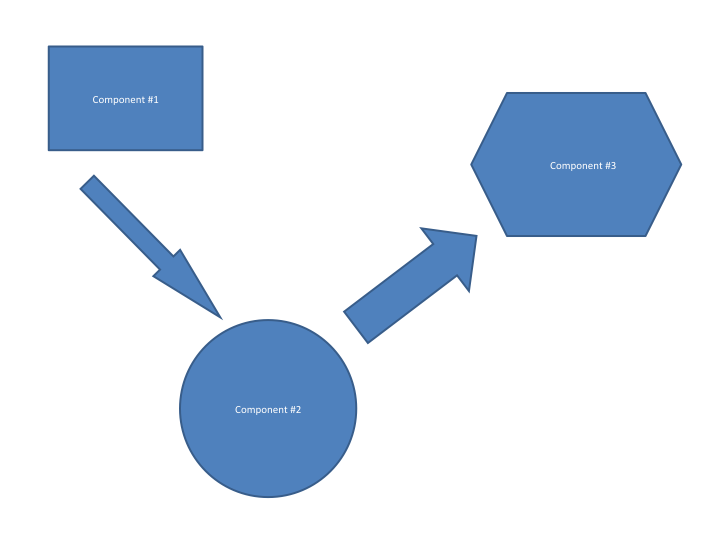
\includegraphics[width=0.75\textwidth]{./diagram}
\end{center}
\caption{A sample figure .... System Diagram \label{systemdiagram}}
\end{figure}

\subsection{Website}
Describe briefly the role this major component plays in this system. 

\subsection{File Conversion}
The file conversion software converts files between common 3D file types.  It is designed to 
be called from the back end of the website.

Table \ref{table:suportedfiletypes} lists the minimum file types supported.  More may be supported, but those listed are the minimum needed to support the majority of common file types.  
Models created in most common Computer Aided Design software can export to some of the input file types.

\begin{table}[!h]
    \centering
    \begin{tabular}{| c | c |}
        \hline
        Input file type & Output file type \\
        \hline
        .fbx & .fbx \\
        .dae & .dae \\
        .blend & .obj \\ 
        .obj & .stl \\
        .stl & .ply \\
        .ply & \\
        \hline
    \end{tabular}
    \caption{Supported File Types}
    \label{table:suportedfiletypes}
\end{table}

\section{Technologies Overview}
This section should contain a list of specific technologies used to
develop the system.  The list should contain the name of the
technology, brief description, link to reference material for further
understanding, and briefly how/where/why it was used in the system.
See Table~\ref{somenumbers}.  This is a floating table environment.
\LaTeX\ will try to put it close to where it was typeset but will not
allow the table to be split.

\begin{table}[tbh]
\caption{A sample Table ... some numbers. \label{somenumbers}}
\begin{center}
\begin{tabular}{|r|l|}
  \hline
  7C0 & hexadecimal \\
  3700 & octal \\ \cline{2-2}
  11111000000 & binary \\
  \hline \hline
  1984 & decimal \\
  \hline
\end{tabular}
\end{center}
\end{table}


 \section{Architecture and System Design}
This is where you will place the overall system design and the architecture.   This section will be very detailed and should be image rich.  There is the old phrase {\it a picture is worth a thousand words}, in this class it could be worth hundreds of points (well if you sum up over the entire team).   One needs to enter the design and why a particular design has been done.   THIS IS THE CORE OF THE COURSE.    
 
 
 {\it It is important for you to say why as much as what.   }
 
   \subsection{Design Selection}
 Failed designs, design ideas, rejected designs here.
 
 \subsection{Data Structures and Algorithms}
 Describe the special data structures and any special algorithms.
 
 \subsection{Data Flow}
 
 \subsection{Communications}
 
 \subsection{Classes}
 
 \subsection{UML}
 
 \subsection{UX}
 
 \subsection{UI}
 
 \subsection{MVVM, etc}

 \section{Website}

 \section{File Conversion}

    \subsection{Overview}
    \paragraph{}
    A major tool in the project is the File Conversion Software.  
    The file conversion software aims to read in many different 3D model file types (.fbx, .obj, .dae, ...) and convert them to another desired 3D file type.  
    A brief listing of suported file types is in table \ref{table:suportedfiletypes}.

    \paragraph{}
    This tool is intended to be used on the back end of the website.  Whenever a user uploads a file, it can be converted to a common file type, using this tool.
    When the user requests a download on an AR device, the type may be different than what is stored.  Therefore, the tool will be used to convert the file before
    it is sent to the user.

    \paragraph{}
    Since this tool is intended to be used on the backend of a website, it is appropriate to use a command line interface.  
    The flags that can be passed to the program are listed below:

    \begin{table}[h]
        \centering
        \begin{tabular}{l  l}
            -i & Input file name (can specify full path), infers the input file type from the name \\
            -o & Name (or full path) to write the converted file, infers the export file type from the name \\
            -odir & The path to the directory, the file name is inferred from the input file name \\
            -t & The file type (.fbx, .obj, .dae, ...) to export to
        \end{tabular}
    \end{table}

    Note the -t flag is only needed when using the -odir flag.  The -odir just specifies which directory to write to, but not the file type.
    Therefore, more information is needed in order to export to a file.  The -o flag will parse the file name and extract the file type from the -i file name.

    An example command to run:

    \begin{center}
        .\textbackslash FileConversion.exe -i C:\textbackslash SomePath\textbackslash someFile.obj -t fbx -odir C:\textbackslash SomeOtherPath\textbackslash
    \end{center}

    This will convert a file named someFile.obj located at C:\textbackslash SomePath\textbackslash  to an FBX file named someFile.fbx located at 
    C:\textbackslash SomeOtherPath\textbackslash

    \subsection{Technologies Used}

    The code for the file conversion toolset is written in C++.  There are two main external libraries used:
    \begin{itemize}
        \item Open Asset Import Library (assimp)
        \begin{itemize}
            \item \url{http://assimp.org/main_downloads.html}
        \end{itemize}

        \item FBX SDK
        \begin{itemize}
            \item \url{http://usa.autodesk.com/adsk/servlet/pc/item?siteID=123112&id=26416244}
        \end{itemize}
    \end{itemize}

    Multiple librarires are needed to support the file types that are necessary for common AR rendering.  In the Microsoft Hololens, the default
    3D viewer supports FBX files very easily.  Therefore, it was decided that the conversion software needed to export to FBX.  The best tool to do 
    so is the FBX SDK, since FBX is a propriatary file format from Autodesk.  However, the FBX SDK has a very limited range of file types it will read and write.
    Therefore, the Open Asset Import Library is used to better support a wide array of file types.  So in using assimp and the FBX SDK together,
    the converison software can support a wide range of both import and export file types.

    \subsection{Data Flow}
        There are four main paths data can flow.
        \begin{itemize}
            \item assimp
            \begin{itemize}
                \item import and export all with the assimp library
            \end{itemize}
            
            \item FBX SDK
            \begin{itemize}
                \item import and export all with the FBX SDK library
            \end{itemize}

            \item assimp $\rightarrow$ FBX SDK
            \begin{itemize}
                \item import with assimp, export to temporary file type
                \item import temporary file with FBX SDK, export to final file 
            \end{itemize}

            \item FBX SDK $\rightarrow$ assimp
            \begin{itemize}
                \item import with FBX SDK, export to temporary file type
                \item import temporary file with assimp, export to final file 
            \end{itemize}
        \end{itemize}
        
        This outlines that the program tries to use a single library to convert the file before using multiple.  If a single library is unable to 
        read and write the needed formats, it tries to import with one, export to a temporary format, and export with the other.  An example of 
        using a single library is if a user wants to read a .obj and write to a .fbx.  The FBX SDK can handle reading and writing those particular file
        types, so it will be used ot do the conversion.  An example of needing to use both libraries is if a user wants to convert a .ply to a .fbx.
        Assimp can read .ply files, but cannot write to .fbx.  The FBX SDK can write to .fbx files but not read .ply.  Therefore, assimp is used to 
        read the .ply, write to a .dae (common file type).  The FBX SDK then reads the .dae and writes to a .fbx.

    \subsection{Design Details}

    \subsubsection{Overview}

    The file converison software is written in C++.  The structure of the program is object oriented, where classes are defined where the functionality needed
    in the program is defined.  Instances of the classes will be created when needed.  
    The high level view of the program is:
    \begin{enumerate}
        \item Parse command line arguments
        \item Convert the file
        \item Print error messages if errors occured
    \end{enumerate}

    The parsing the command line arguments section may fail if the user does not supply the correct arguments.  A flag is set after parsing to indicate
    whether the correct arguments were supplied.  If an error occurrs during file conversion, the error will be denoted by an integer error code.  
    During file conversion, if a single library could not convert it on its own, an extra file will be created as an intermediate file.

    \subsubsection{Code Structure}
    The file conversion software is broken into two main sections: parameter parsing and file conversion.

    \paragraph{Parameter Parsing}
    \hfill \break
    The parameter parsing code is in a class called ParseParameters.  ParseParameters has a constructor that takes the number of command line arguments, 
    and the command line arguments.  It will parse the values needed out into member variables that are public.  It will ignore invalid arguments,
    and print a usage statement if the correct arguments are not supplied.  When printing the useage statement, cout is used to write to standard out.

    After processing the command line arguments, the member variables in the class will be set with the appropriate information.  The member variables are:

    \begin{tabular}{l l}
        \centering
        success & bool \\
        & True if the needed information is set, false otherwise \\

        inputFile & string \\
        & The name/path of the file to convert \\

        outputFile & string \\
        & The name/path of the file to export to \\

        fileExtention & string \\
        & The file extention of the output file
    \end{tabular}

    If the success variable is false, the other member variables possibly have bad data that should not be used.

    \paragraph{File Conversion}
    \hfill \break
    The file conversion portion of the progarm is the meat of the functionality.  It takes an input file, and tries to convert it to the file type requested.
    This seciton implements the two libraries.  Each library is implemented in a class inherited from an abstract AbstractConverter converter class.  The two 
    library implementation classes are called AssimpConverter and FBXConverter.  A class named FileConverter contains the logic on determining which 
    library/libraries to use when converting the file.

    \subparagraph{AbstractConverter}
    \hfill \break
    The AbstractConverter is an abstract class that acts like an interface for the child classes.  The abstract methods are:
    \begin{itemize}
        \item SupportsInputFileType
        \begin{itemize}
            \item Return true if the converter can read in a file with a given file type
        \end{itemize}

        \item SupportsOutputFileType
        \begin{itemize}
            \item Return true if the converter can write to a file with a given type
        \end{itemize}

        \item ConvertFile
        \begin{itemize}
            \item Performs the file conversion
        \end{itemize}
    \end{itemize}

    An emum is defined, called Result, that provides a more self documenting way to return information from functions.  Values less than zero are errors, while
    value greater than zero are successes.  The levels of the enum are:
    
    \begin{tabular}{l l}
        \centering
        Failed &\\
        IOError &\\
        SceneNotLoaded &\\
        NotInitialized &\\
        FileTypeNotSupported &\\
        Success &
    \end{tabular}

    \subparagraph{AssimpConverter}
    \hfill \break
    The AssimpConverter inherits from the AbstractConverter and uses the Open Asset Import Library for file conversion.  
    The file type supported methods are implementd by adding the supported file types to a set, and checking whether the questionable type is in the set.
    The list of file types supported is taken from the Open Asset Import Library website's list of supported input file types.  
    The output file types list comes from the same location.
    When converting a file, optimizations may be performed on the file to remove unnecessary/duplicate information.  For example, when importing a file, 
    repeatedverticies in the meshes will be condensed into one, to help reduce the size of the file.

    \subparagraph{FBXConverter}
    \hfill \break
    The FBXConverter inherits the AbstractConverter and uses the FBX SDK to import and export files.
    THe file type input and output lists are derived from the FBX SDK website.

    \subparagraph{FileConverter}
    \hfill \break
    The FileConverter looks at the input and output file types, and determines which library/libraries needed to convert the file.
    It tries see if a single library can do the conversion.  If not, then both libraries are used by exporting from one into a 
    temporary file (.dae) and converting that to the final file type. After comparing the read/write lists between the libraries,
    the DAE file type was common between the two, and included features that other file types did not.  Therefore, it was chosen
    to have DAE as the common intermediate file type.

 \begin{comment}
    \section{Major Component \#1 }

    {\bf If the following makes sense, use this outline, if not then modify the outline}


    This section is used to describe the design details for each of the major components 
    in the system.    Note that this chapter is critical for all tracks.  Research tracks would do experimental design here where other tracks would include the engineering design aspects.    This section is not brief and requires the necessary detail that 
    can be used by the reader to truly understand the architecture and implementation 
    details without having to dig into the code.    Sample algorithm:  Algorithm~\ref{alg1}.  This algorithm environment is automatically placed - meaning it floats.   You don't have to worry about placement or numbering.  

    \begin{algorithm} [tbh]                     % enter the algorithm environment
    \caption{Calculate $y = x^n$}          % give the algorithm a caption
    \label{alg1}                           % and a label for \ref{} commands later in the document
    \begin{algorithmic}                    % enter the algorithmic environment
        \REQUIRE $n \geq 0 \vee x \neq 0$
        \ENSURE $y = x^n$
        \STATE $y \Leftarrow 1$
        \IF{$n < 0$}
            \STATE $X \Leftarrow 1 / x$
            \STATE $N \Leftarrow -n$
        \ELSE
            \STATE $X \Leftarrow x$
            \STATE $N \Leftarrow n$
        \ENDIF
        \WHILE{$N \neq 0$}
            \IF{$N$ is even}
                \STATE $X \Leftarrow X \times X$
                \STATE $N \Leftarrow N / 2$
            \ELSE[$N$ is odd]
                \STATE $y \Leftarrow y \times X$
                \STATE $N \Leftarrow N - 1$
            \ENDIF
        \ENDWHILE
    \end{algorithmic}
    \end{algorithm}
    Citations look like~\cite{Choset:2005:PRM, arkin2009governing, lavalle2006}  and~\cite{wiki:asimo,lumelsky:1987, nolfi2000evolutionary}.  These are done automatically.  Just fill in the database {\tt designrefs.bib} using the same field structure as the other entries.  Then pdflatex the document, bibtex the document and pdflatex twice again.  The first pdflatex creates requests for bibliography entries.
    The bibtex extracts and formats the requested entries.  The next pdflatex puts them in order and assigns labels.  The final pdflatex replaces references in the text with the assigned labels.
    The bibliography is automatically constructed.  
    


    \subsection{Technologies  Used}
    This section provides a list of technologies used for this component.  The details 
    for the technologies have already been provided in the Overview section. 

    \subsection{Component  Overview}
    This section can take the form of a list of features. 

    \subsection{Phase Overview}
    This is an extension of the Phase Overview above, but specific to this component. 
    It is meant to be basically a brief list with space for marking the phase status. 

    \subsection{ Architecture  Diagram}
    It is important to build and maintain an architecture diagram.  However, it may 
    be that a component is best described visually with a data flow diagram. 


    \subsection{Data Flow Diagram}
    It is important to build and maintain a data flow diagram.  However, it may be 
    that a component is best described visually with an architecture diagram. 


    \subsection{Design Details}
    This is where the details are presented and may contain subsections.   Here is an example code listing:
    \begin{lstlisting}
    #include <stdio.h>
    #define N 10
    /* Block
    * comment */
    
    int main()
    {
        int i;
    
        // Line comment.
        puts("Hello world!");
    
        for (i = 0; i < N; i++)
        {
            puts("LaTeX is also great for programmers!");
        }
    
        return 0;
    }
    \end{lstlisting}
    This code listing is not floating or automatically numbered.  If you want auto-numbering, but it in the algorithm environment (not algorithmic however) shown above.

\end{comment}
  %% All tracks
% !TEX root = DesignDocument.tex


\chapter{Testing}
\label{ch:testing}

% This section describes the approach taken with regard to system and unit testing.    This chapter does not describe the outcome of those tests.    

\section{Overview}
\tab The testing approach is based on automated unit testing where available and manual testing with instructional testing steps recorded. Website testing, file conversion testing, mobile application testing, and component integration testing are all recorded and documented separately. The purpose of the product tests is to ensure that the features described in the user stories and project specification are met and work as intended. The manual tests for each user story are described below.

\section{Dependencies}
\tab The main testing framework for the Azure website is Microsoft's C\# testing framework. The file conversion needs no external testing framework as it is tested manually for accuracy. The database schema and implementation is provided by the Microsoft Entity Framework package, in which stable releases are guaranteed functional, however testing is done by verifying state persistence across publications.


 \section{Website}

 \subsection{Overview}
 \paragraph{}
 The website is a hosting service for uploading, downloading and managing the users files. Microsoft's ASP.NET MVC was used to create the website and Azure was used for its web hosting and file storage tools.
 
 \paragraph{}
 Users can create an account to store and share 3D models with other users. Once a user has an account, they can upload a 3D model as one of the websites supported file types. A user can download the model as any of the supported file types or generate a QR code that can be used for quick download using the mobile app or any other QR code readers.

\subsection{User Interface}
The user interface was designed to be very simple. The UI is comprised of four main pages with a navigation bar to get the pages
    \paragraph{Public Content Page}

        \begin{figure}[H]
        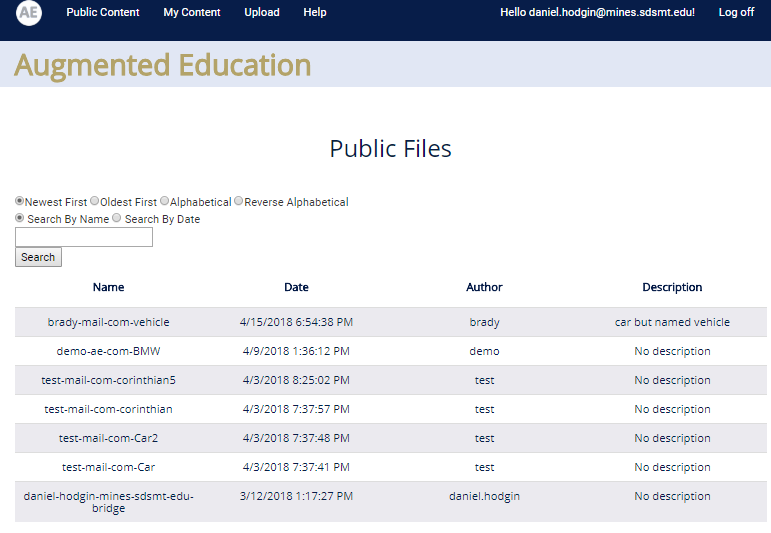
\includegraphics[width=0.5\textwidth]{Web/PublicPage}
        \centering
        \caption{Public Content Page}
        \label{fig:PublicContent}
        \end{figure}

        This is the main landing page for the website. From here users are able to browse the public files to download and generate QR code. Users do not need to be signed in or have an account to access the information on this page.

    \paragraph{My Content Page}
        \begin{figure}[H]
        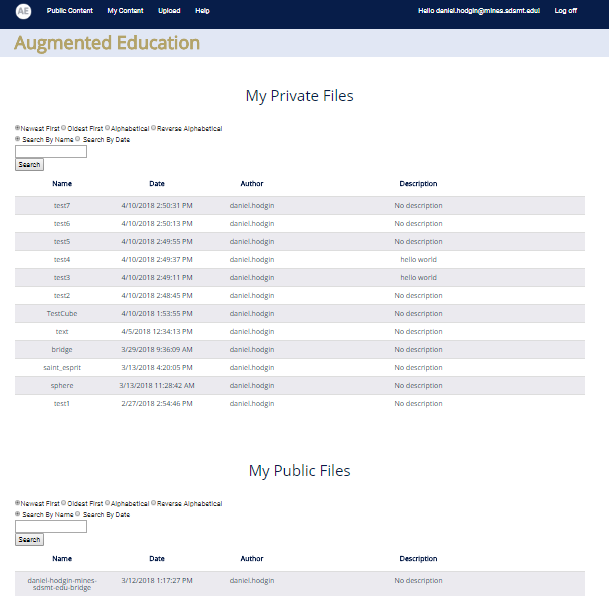
\includegraphics[width=0.5\textwidth]{Web/MyContent}
        \centering
        \caption{My Content Page}
        \label{fig:MyContent}
        \end{figure}

        This page will display all of the content that a user has uploaded. Here a user can browse their private and public files to download and generate QR codes. Users also have the ability to delete files. Users must have an account to access this page.

    \paragraph{Upload Page}
        \begin{figure}[H]
        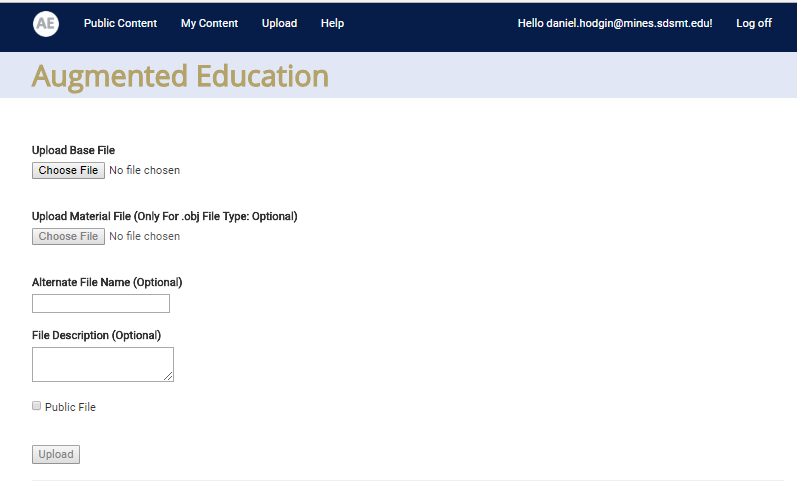
\includegraphics[width=0.5\textwidth]{Web/Upload}
        \centering
        \caption{Upload Page}
        \label{fig:UploadPage}
        \end{figure}

        This page will allow users to upload 3D models. Users can upload a material file if it is an OBJ file. The user can add a description, specify an alternate name, and make the file public. Users must have an account and be signed in to access this page.

    \paragraph{Help Page}
        \begin{figure}[H]
        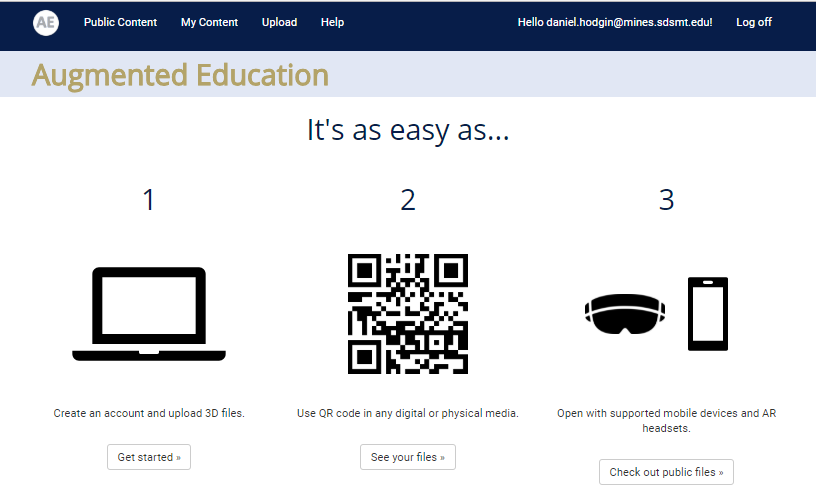
\includegraphics[width=0.5\textwidth]{Web/Help}
        \centering
        \caption{Upload Page}
        \label{fig:HelpPage}
        \end{figure}
    
        This page just gives a simple tutorial on how to uses the website.

\subsection{Technologies Used}

    As stated earlier in this document, this product is making use
    of the Microsoft environment for its tools. Below is an in-depth 
    breakdown of the tools currently being used:

    \begin{itemize}
    \item ASP.NET MVC
    \begin{itemize}
        \item An MVC web architecture, where the backend logic is written in controller classes
        that send and receive data from the client.
        \item It allows for dynamic html pages using a Razor syntax. Razor allows
        you to embed C\# Code into the html and execute logic.
    \end{itemize}
    
    \item Azure
        \begin{itemize}
            \item Microsoft cloud hosting services.
            \item Allows for simple database and web hosting.
            \item Paid features are offered free to students.
        \end{itemize}
    \end{itemize}

    These tools make up the core development of this website. The website is also
    making use of other smaller packages to handles user authentication and database management.

    The website also implements the file conversion software that is described later.
    The file conversion was written in C++, so it couldn't be compiled with the website.
    The workaround was that the file conversion was compiled into an executable that can be used through a system command to convert the file.


    \subsection{Data Flow}
    The website acts as an intermediary between the user and the cloud. Data flow for the website can be broken into a upload and download data flow.

    \paragraph{Upload Data Flow}
    \begin{itemize}
        \item Once a user upload a file it is temporarily save on the server.
        \item If the file is not a FBX file it is converted to a FBX file.
        \item The file is then uploaded to Azure blob storage for long term storage.
        \item The file on the server is then deleted on a sucessful upload to Azure.
    \end{itemize}

    \paragraph{Download Data Flow}
    \begin{itemize}
        \item When a user requests to download a file or generate a QR code, the file name and type is sent to the server.
        \item The server pulls the file from Azure and temporarily save it to the server.
        \item If a download is requested, it does a conversion if nessessary and send the file to the user.
        \item If a QR code is generated, it does a conversion if nessessary and then saves it back to Azure storage and returns a link to the file in Azure embedded in a QR code.
        \item 
    \end{itemize}


\subsection{Design Details}

    \subsubsection{Overview}

    The website was written in C\# with the ASP.NET MVC framework. The main logic
    of the website are contained in two controllers
    \begin{itemize}
        \item Upload Controller
        \begin{itemize}
            \item Handles upload from client to the server.
            \item Uses File Conversion executable to convert to .fbx
            \item Stores file on the web.
        \end{itemize}
        \item Download
        \begin{itemize}
            \item Uploads Model tag from client to server.
            \item Finds associated store model.
            \item Returns model to the client.
        \end{itemize}
    \end{itemize}

    \subsubsection{Code Structure}
    As stated before the website is using ASP.NET MVC framework. 
    The logic happens in the controllers and is split up into the upload and download controller.
    
    \paragraph{Parameter Passing}
    \hfill \break
    The main functions that are being used are the upload and download function.
    
    \begin{itemize}
        \item Upload Function
        \begin{itemize}
           \item HttpPostedFileBase - http message sent from client to server containing the file
           \item The message is parsed to retrieve the file and save to the web.
        \end{itemize}

        \item Download Function
        \begin{itemize}
            \item input string ModelTag - string containing the reference tag to the model.
            \item output httpresponse - http message sent from server to client containing the file. 
        \end{itemize}
    \end{itemize}

% !TEX root = DesignDocument.tex

\section{File Conversion Testing}
    The file conversion was manually tested using a variety of inputs to ensure robust and consistent performance. As there are two libraries (assimp and FBX SDK), they were both manually tested for simple functionality as they were implemented. Manual tests included sending through file types that could be inputs for assimp and making sure that the files made it to the FBX section and output the correct file format (FBX). Some of the input file types tested included common and expect file types such such as STL, OBJ, DAE etc. Unsupported file types were also tested and appropriate errors from the conversion libraries were received. The file types supported by the system are available in Table \ref{tab:suportedfiletypes}. Large files were also tested to gauge how long the system could take to process files of different sizes. There are certain limitations on the HoloLens hardware regarding file size and complexity. Users are properly notified of these limitations by the HoloLens platform should they be an issue. The HoloLens limitations are not formerly noted here as they are already anticipated to change with future updates.  

    Files with embedded textures were also tested to ensure textures get converted with the file. With the file types tested, such as OBJ and FBX, the textures converted with the files as expected. The HoloLens default 3D file viewer does not currently support colors or textures, thus these features have not yet been able to be tested.

    Test files of varying complexity were gathered from a variety of sources to ensure maximum coverage by the Augmented Education platform. The following files comprised the original test group used to ensure proper conversion to a FBX format and rendering on the Microsoft HoloLens:
    \begin{itemize}
        \item An OBJ sphere generated in Maple.
        \item An FBX column provided by Dr. Brent Deschamp of SD Mines.
        \item An OBJ sine wave generated in Maple.
    \end{itemize} 
    
    A number of files of varying format type from \url{http://free3d.com} were also tested. These sample files included a car, building, spaceship, Batman, and other unique files. 
    
    Cheldon was also able to receive large sample architectural files in FBX format from a relative. One architectural file rendered in the HoloLens, but the other two were too large to be supported by the device's current limitation for meshes and vertices able to be rendered in the viewer.

    Conversion examples can be seen in Figures \ref{Car-FBX}, \ref{Car-OBJ}, and \ref{Car-STL}.  
    
    In Figure \ref{Car-FBX}, a 3D model for a car in FBX format was acquired. This file was used to test conversion to OBJ format, the result of which can be seen in Figure \ref{Car-OBJ}. Figure \ref{Car-STL} is an STL file generated from the FBX file, using a DAE file as an intermediate format between the FBX SDK and assimp libraries. The STL file does not contain the colors or smooth surfaces that are present in the other file types, which is a limitation of the STL file format. This system works for converting STL $\rightarrow$ FBX as well, but the colors would not be present in the final file because that information is not contained in the STL. 
    
\begin{figure}[H]
    \centering
    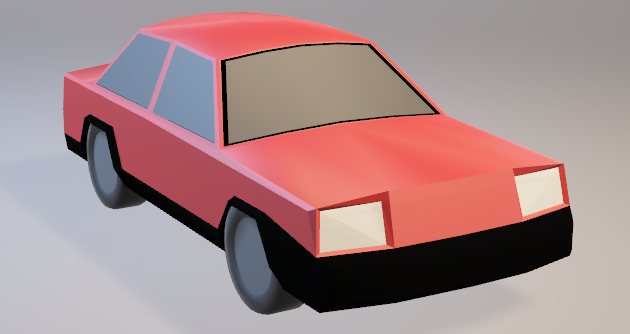
\includegraphics[width=\textwidth]{Car-FBX.png}
    \caption{Car FBX File}
    \label{Car-FBX}
\end{figure}

\begin{figure}[H]
    \centering
    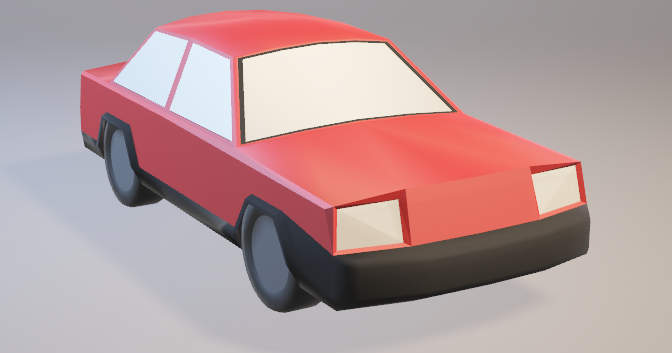
\includegraphics[width=\textwidth]{Car-OBJ.png}
    \caption{Car OBJ File}
    \label{Car-OBJ}
\end{figure}

\begin{figure}[H]
    \centering
    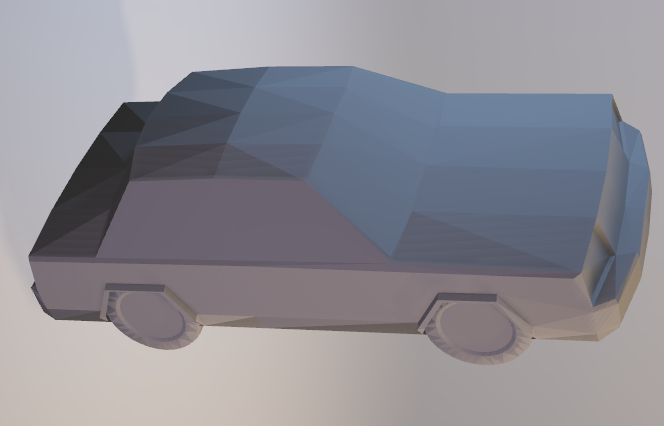
\includegraphics[width=\textwidth]{Car-STL.png}
    \caption{Car STL File}
    \label{Car-STL}
\end{figure}



\section{Mobile Testing}
    Testing for the mobile app was primarily done manually. This is because most testing was done on visualizing files and verifying the app performed as expected.  It was also verifying that HTTP packets were as expected going to and from the phone.

    When error messages are printed to the user of the app, a toast is displayed.  A toast is the small box that pops up on the lower section of the screen.

    \subsection{Files}
        A variety of files were used throughout development to test functionality of the app. Some sample files were found on \url{https://free3d.com}. Some files were provided from Dr. Deschamp and others were generated in Maple. Different files were used to test that colors were working both in the MTL and as PNGs. Additionally, large and small files were tested to see how the app reacted to more complex files. The BMW file seen below is an example of a complex file that doesn't render well in the app and demonstrates the limitations of the app.
        
        \subsubsection{Colors}
        
            A major feature requested for the app was to be able to display colors. The example below shows a simple sphere with a proof of concept that colors do work. The car is a more in-depth example that shows multiple colors on the same model.
            
            \begin{figure}[H]
                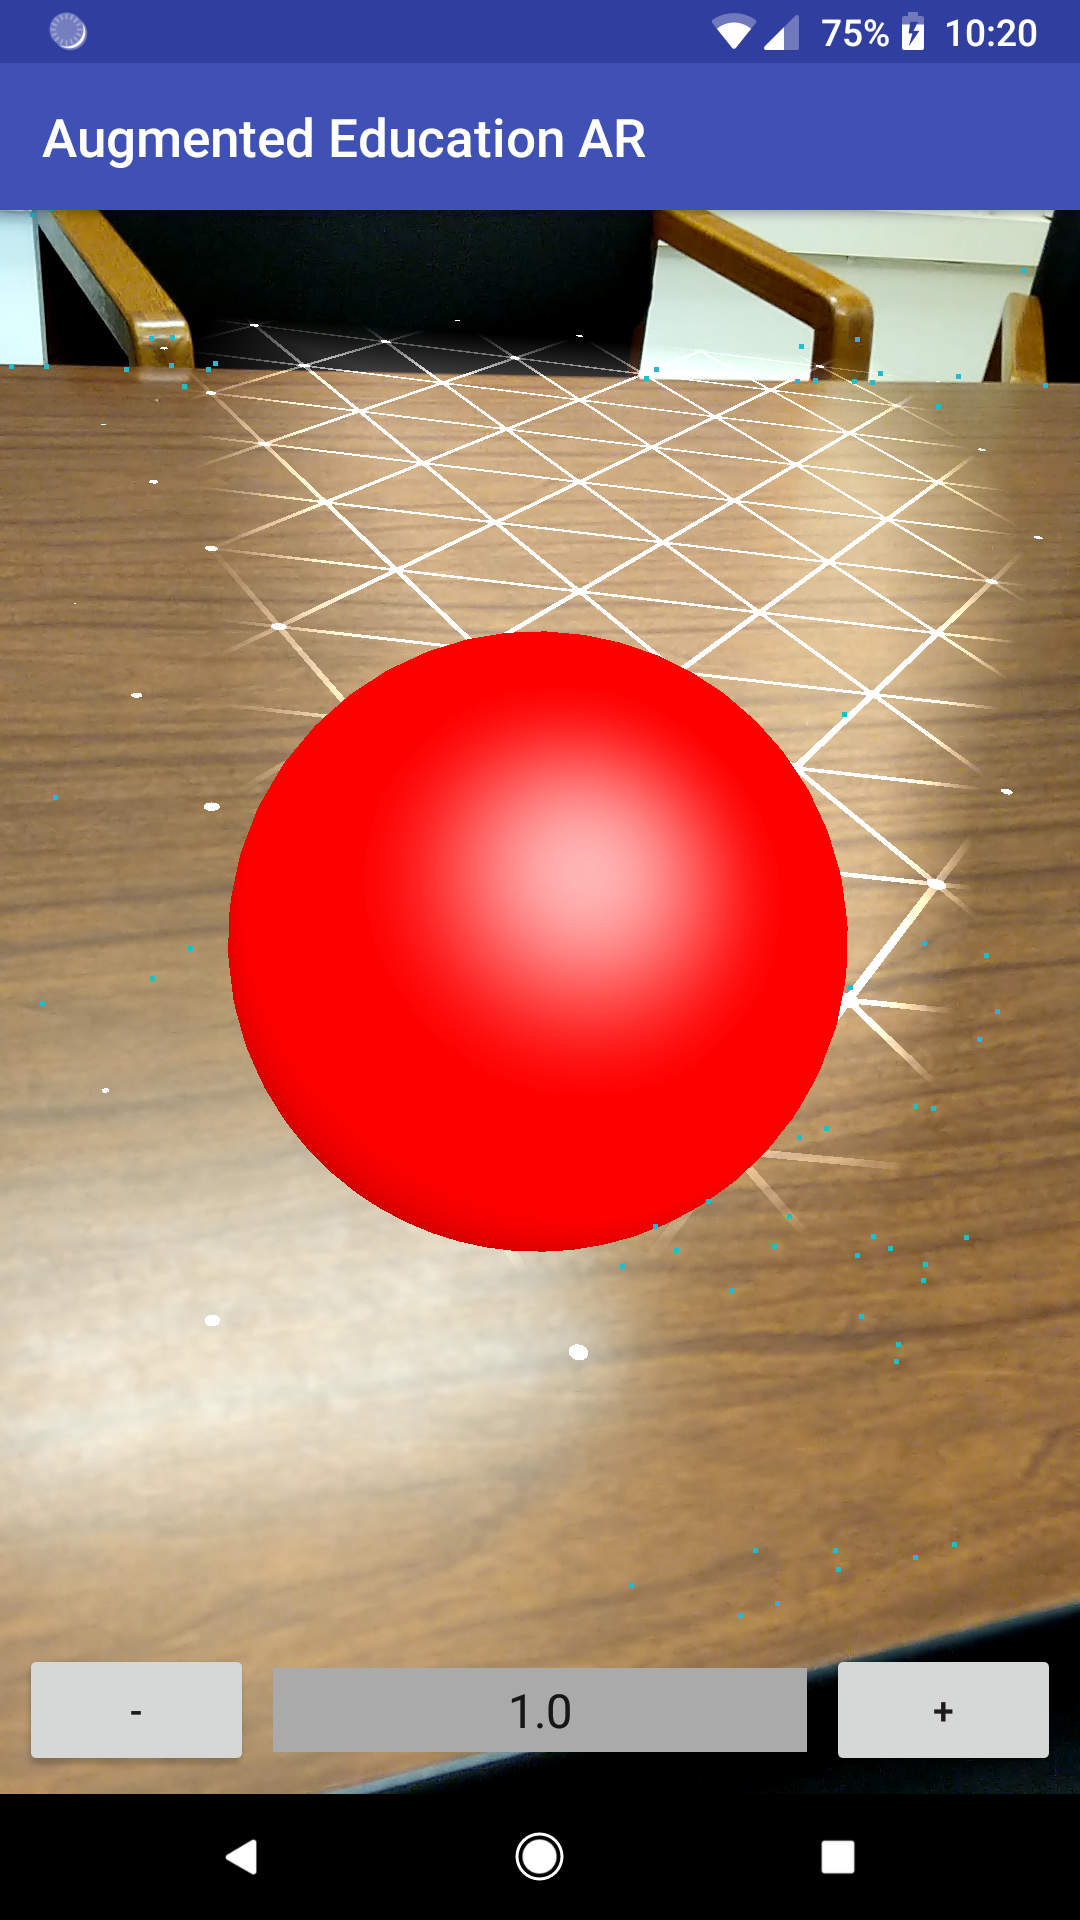
\includegraphics[width=0.5\textwidth]{Mobile/Mobile_RedSphere}
                \centering
                \caption{Colors - Red Sphere}
                \label{fig:mobileRedSphere}
            \end{figure}

            \begin{figure}[H]
                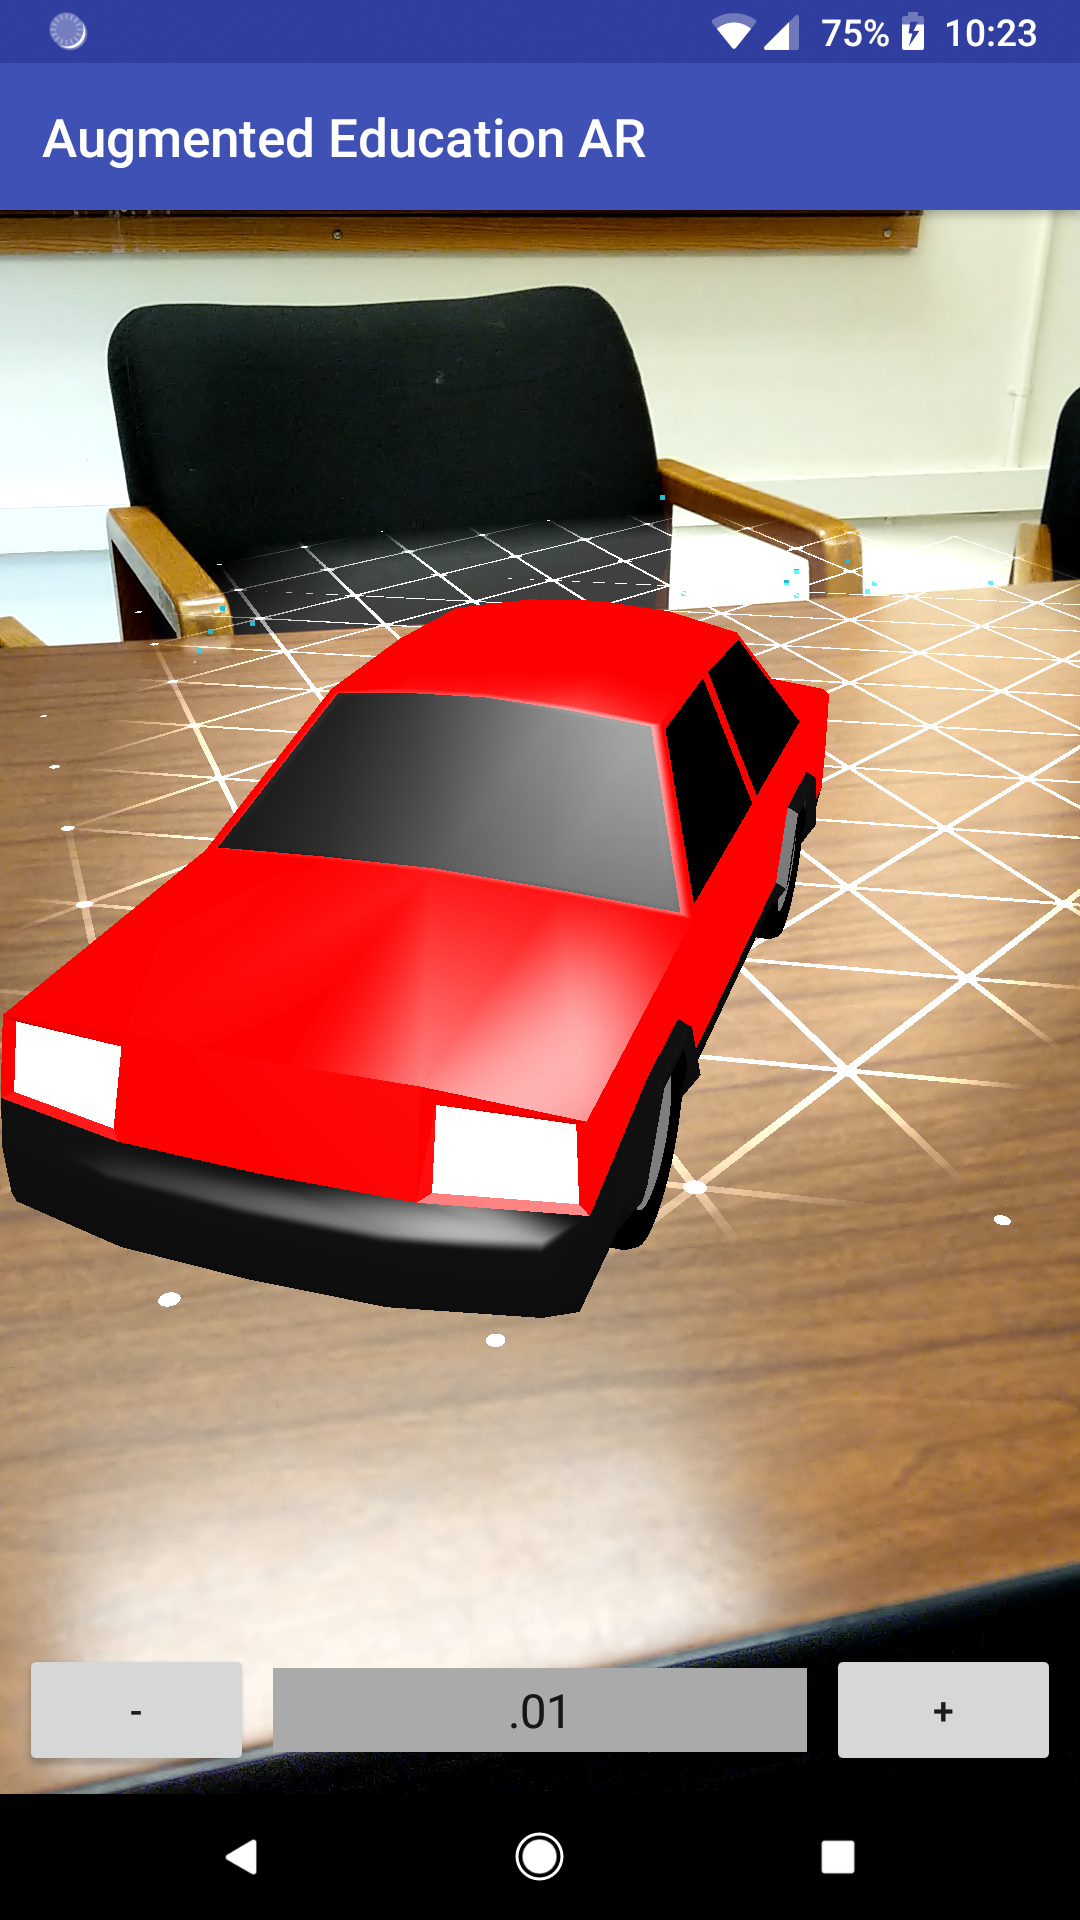
\includegraphics[width=0.5\textwidth]{Mobile/Mobile_Car}
                \centering
                \caption{Colors - Car}
                \label{fig:mobileCar}
            \end{figure}
        
        \subsubsection{Large Files}
        
            One main concern was that 3D files can get large and complex. The BMW is an example of this because it has 51,318 vertices while the sphere only has 2,258. It took a longer amount of time ($\sim$5 seconds) to load this file and it draws poorly, showing a limitation of keeping track of so many vertices.
            \begin{figure}[H]
                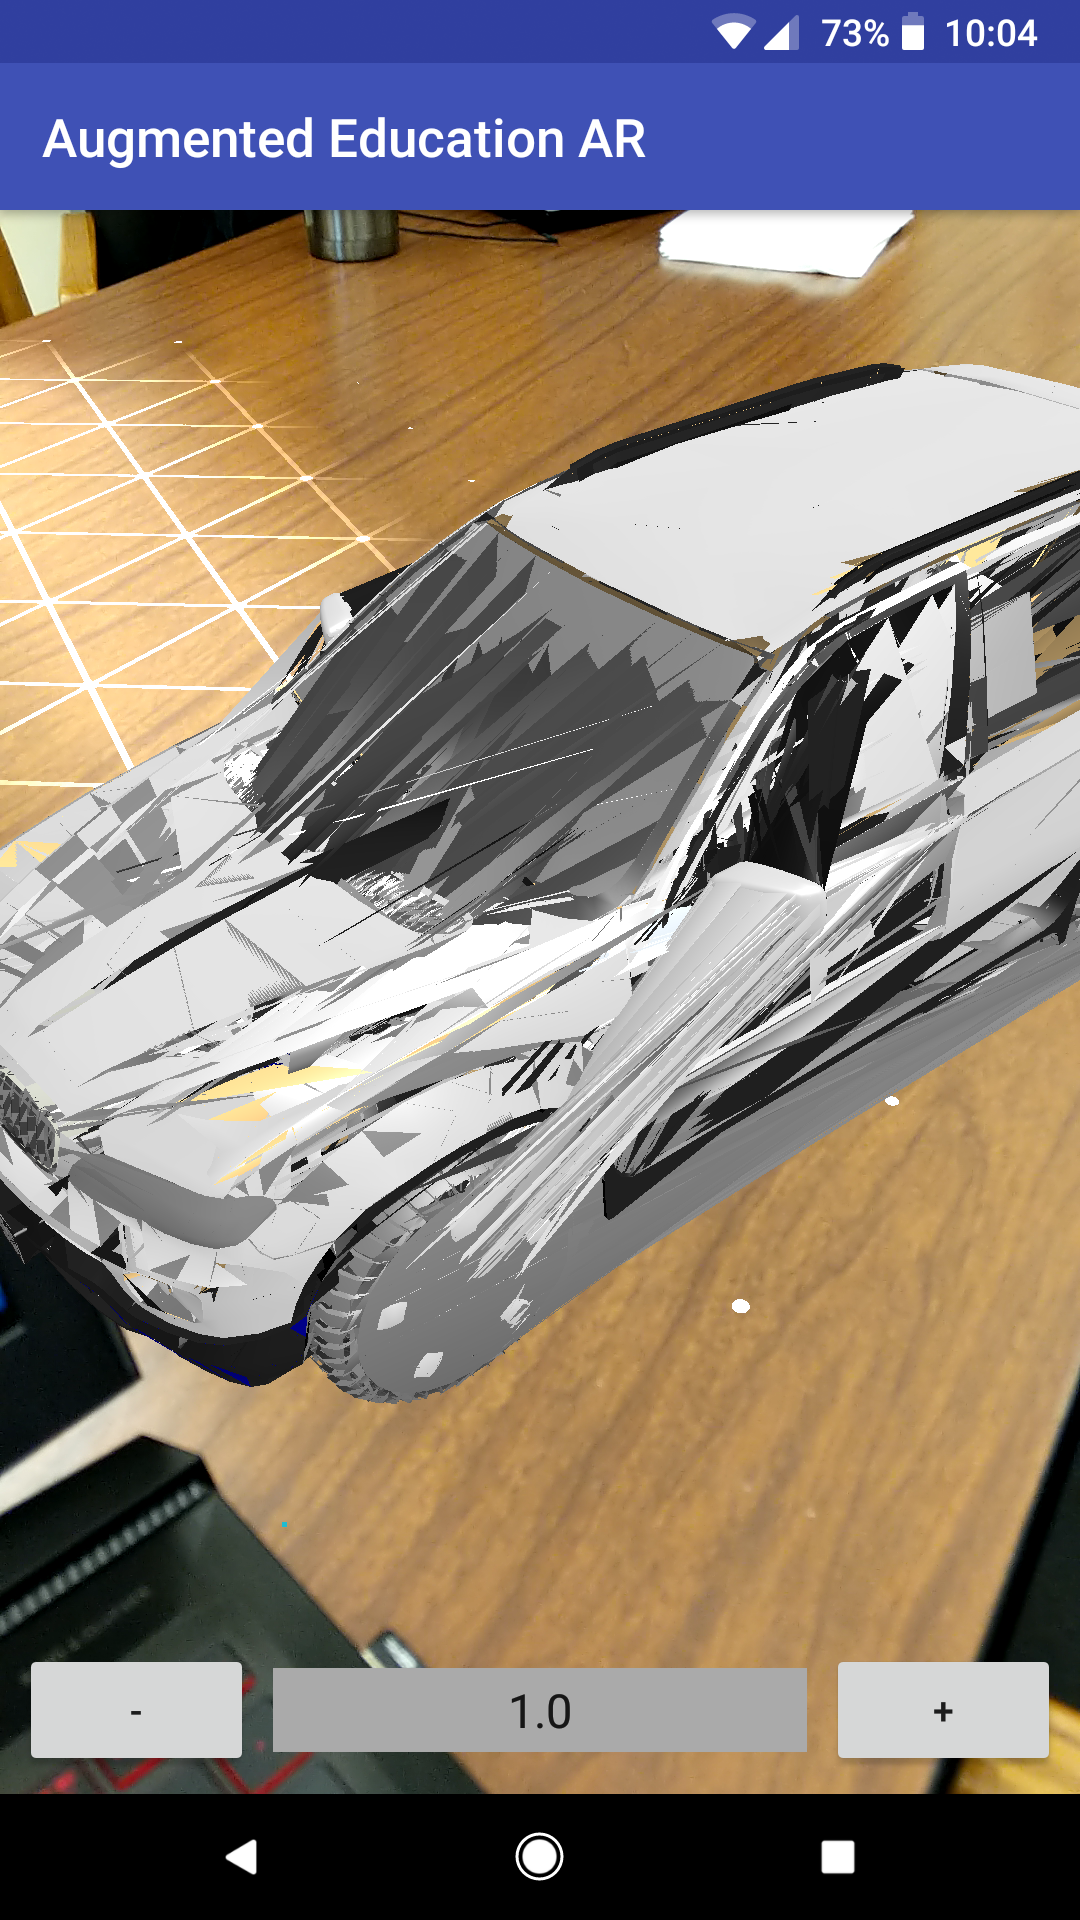
\includegraphics[width=0.5\textwidth]{Mobile/Mobile_BMW}
                \centering
                \caption{Large File - BMW}
                \label{fig:mobileBMW}
            \end{figure}
    
        \subsubsection{Small Files}
            A simple test used especially at the beginning of development to test that models would draw. The sphere is a typical example of something generated from Maple. 
        
            \begin{figure}[H]
                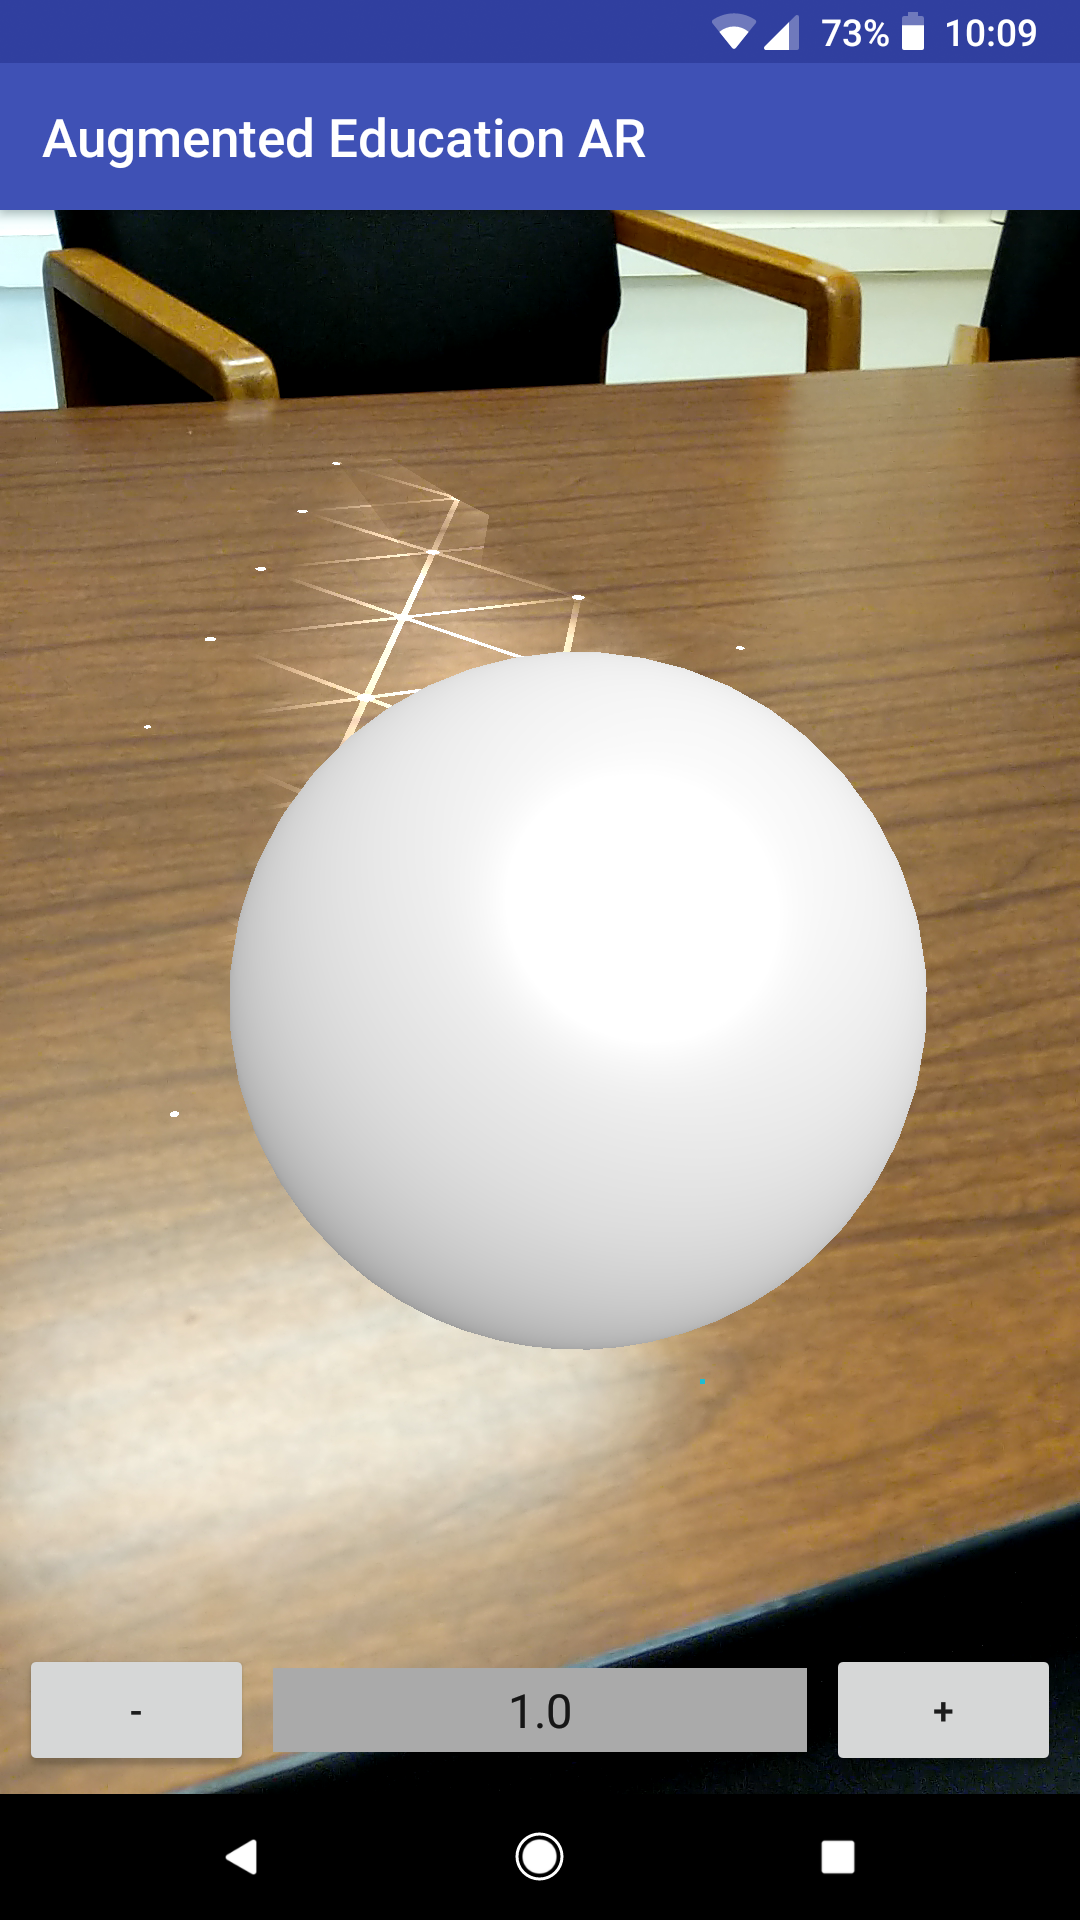
\includegraphics[width=0.5\textwidth]{Mobile/Mobile_Sphere}
                \centering
                \caption{Small File - Sphere}
                \label{fig:mobileSphere}
            \end{figure}
            
        \subsubsection{Embedded Images}
            
            Some 3D modeling software generates OBJ files with PNG textures referenced in the MTL instead of defining RGB values. It was necessary to test that these files were also supported by the app after adding extra functionality for them. Figure \ref{fig:mobileEmbeddedPhone} shows the PNG texture working, but it doesn't match the intended plot perfectly (Figure \ref{fig:mobileEmbeddedWindows}). This is because the app currently does not support drawing multiple images on top of each other yet.
        
            \begin{figure}[H]
                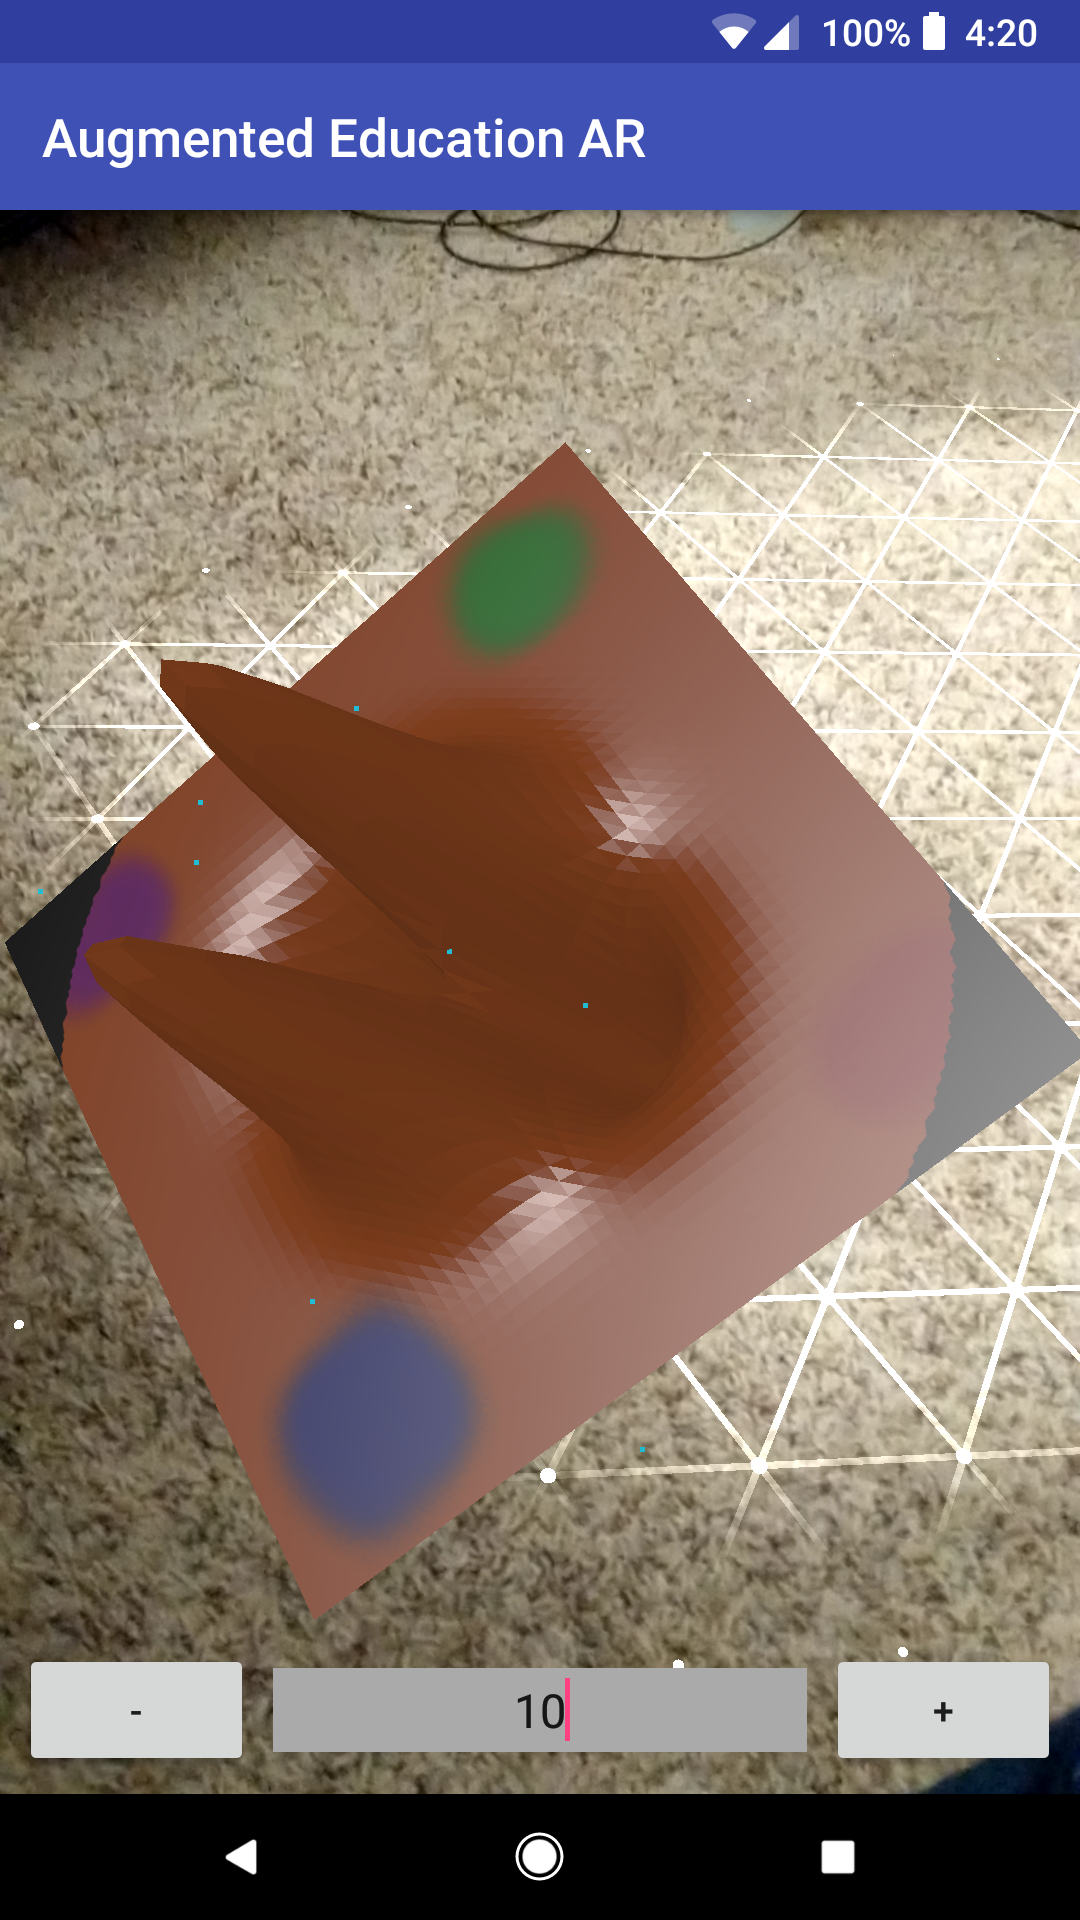
\includegraphics[width=0.5\textwidth]{Mobile/Mobile_ImagesPhone}
                \centering
                \caption{Embedded Image - Viewing on the phone}
                \label{fig:mobileEmbeddedPhone}
            \end{figure}

            \begin{figure}[H]
                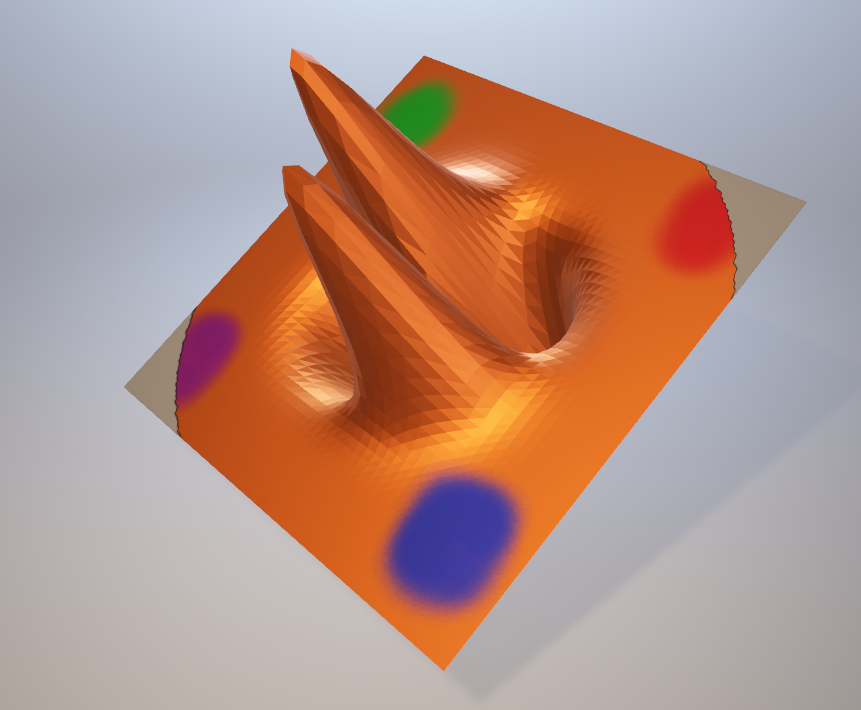
\includegraphics[width=0.5\textwidth]{Mobile/Mobile_ImagesWin}
                \centering
                \caption{Embedded Image - Viewing in the Windows Viewer}
                \label{fig:mobileEmbeddedWindows}
            \end{figure}

        \subsubsection{Scaling}

            Different models scale differently when initially drawn in the app. A scale factor of 1.0 on one model may be too small or too large, making the model difficult to visualize. To remedy this, the app provides an option to increase or decrease the scale factor, as well as change the step so models of different scales can be adjusted properly. Maple models generally need a larger scale factor (approx 3.0) while others like the car need to be adjusted by 0.1 at a time.
        
    \subsection{Web Interface}

        Another major component of the mobile app was the communication with the website.  If the app can display the models, there is little purpose if there is no method to get the models onto the phone.  The web API provided by the web team provides a method for communicating with the website.  It is done using the Volley library, provided by Google.  It abstracts the low level sending/receiving of networking communication away from the developer.  The code for these interfaces in primarily located in the \texttt{WebAccessor} Java class.

        Testing has shown that while the website is on Azure, the responsiveness is not always the best.  It is not infrequent to receive timeout errors on requests.  When this occurs, a message is displayed to the user.
        
        \subsubsection{Endpoints}\label{sec:Mobile_Auth}
        
            The endpoints used by the mobile application allow the app to: authenticate with the website, get a list of owned models, and download a model.  The endpoints were tested using Postman (to make sure the response was what was expected), the Android Studio debugger to make sure the correct fields were set, and a packet capture application to view the actual HTTP message sent from the phone.

            \paragraph{Authenticate}

                The authentication endpoint allowed the user to provide a username and password to get access to the website.  If the user entered valid credentials, an auth token is returned that allows the application to make requests on behalf of the user.  The auth token is used in the other API calls to the server.

                This API call is only performed on the Main Activity screen (the login page).  If a user is not authenticated, the user cannot continue through the app unless they select the Offline Mode button to not perform future web communication tasks.  A success of this component was, if the user supplied valid credentials, a valid auth token was returned.  Otherwise, an error message should be printed.  The testing was performed manually by trying invalid usernames/passwords.  In these cases, the website did not provide a valid auth token.  When correct usernames/passwords were entered, an auth token is returned.

                The Postman view that was used to test the endpoint (on the web side) is shown in Figure \ref{fig:mobilePostmanGetAuthToken}.

                \begin{figure}[H]
                    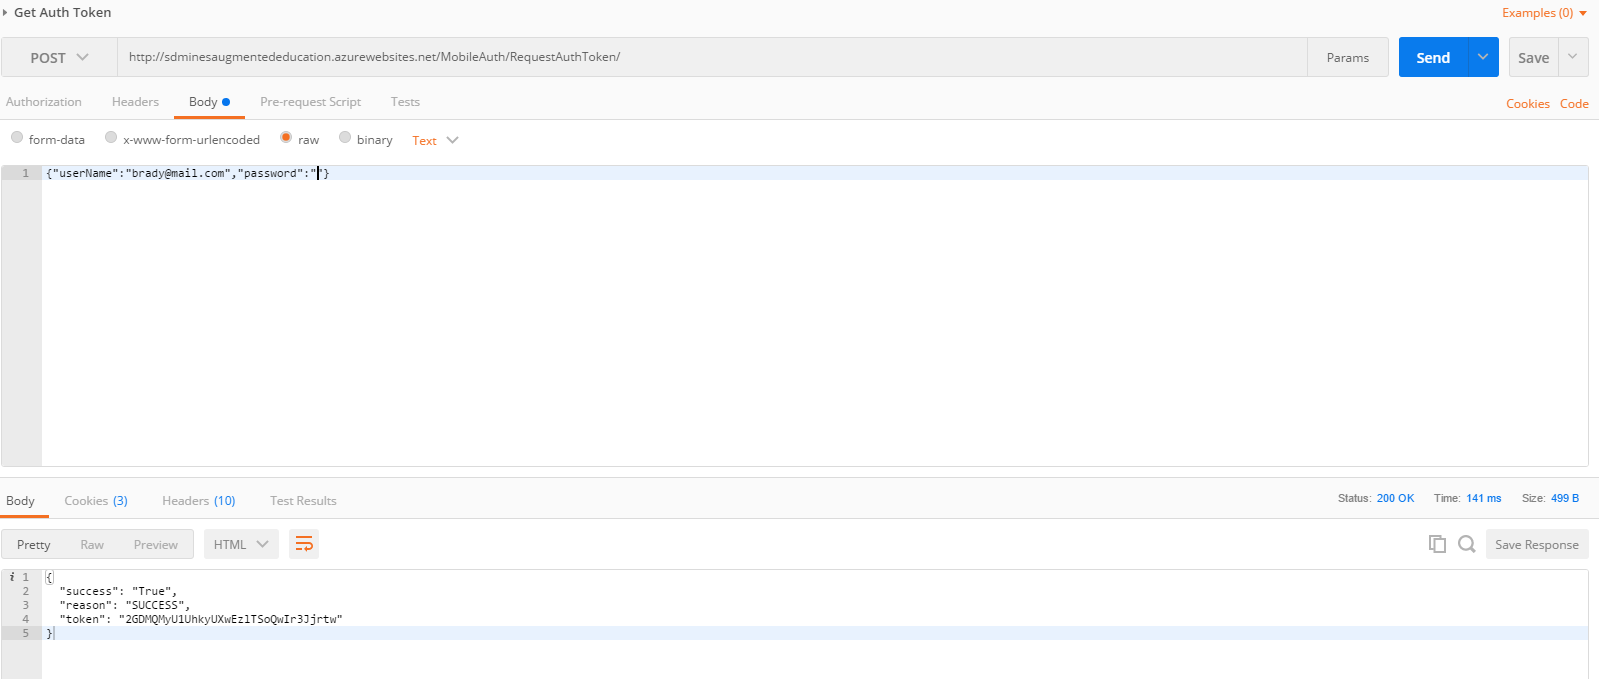
\includegraphics[width=0.75\textwidth]{postman_GetAuthToken}
                    \centering
                    \caption{Postman - Get authentication token}
                    \label{fig:mobilePostmanGetAuthToken}
                \end{figure}
                
            \paragraph{List Models}

                Another endpoint that is used by the mobile device is the one to get a listing of files owned by the user.  Like with the authentication token request, this call was tested manually to ensure the HTTP packets were well formed, and as expected.  Postman was again used to help test.  Figure \ref{fig:mobilePostmanListFiles} shows the Postman setup to send a request for a file listing.  
                
                \begin{figure}[H]
                    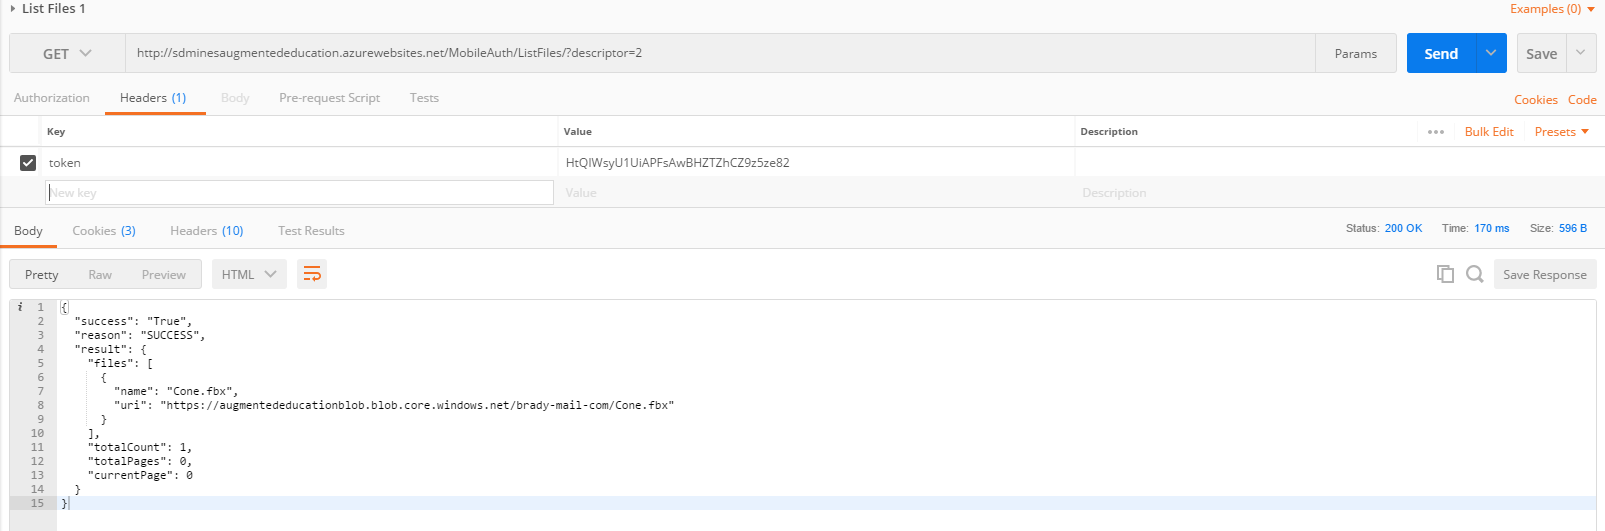
\includegraphics[width=0.75\textwidth]{postman_ListFiles}
                    \centering
                    \caption{Postman - List files}
                    \label{fig:mobilePostmanListFiles}
                \end{figure}
                
                Note, the \texttt{descriptor=} at the end of the URL, as it is used to state which files are desired for download.  An agreement was made between the mobile and web teams on what the levels should be.  There is an enumeration defined in the Java code with more details on the values and meanings.  Testing the different values showed a bug in the web code that always caused an error on the mobile device.  This issue was fixed by the web team.
            
            \paragraph{Download Model}

                Downloading a model includes contacting two endpoints.  One is used to get a temporary link to actually download the file, and the next downloads the file from that URL.  This is used so the phone can store the long term location, and get a temporary active URL to get the file.  Testing for these sections again included using Postman, and using a web browser to facilitate the download.  The Postman settings to get the temporary URL are located in Figure \ref{fig:mobilePostmanDownloadFile}.

                \begin{figure}[H]
                    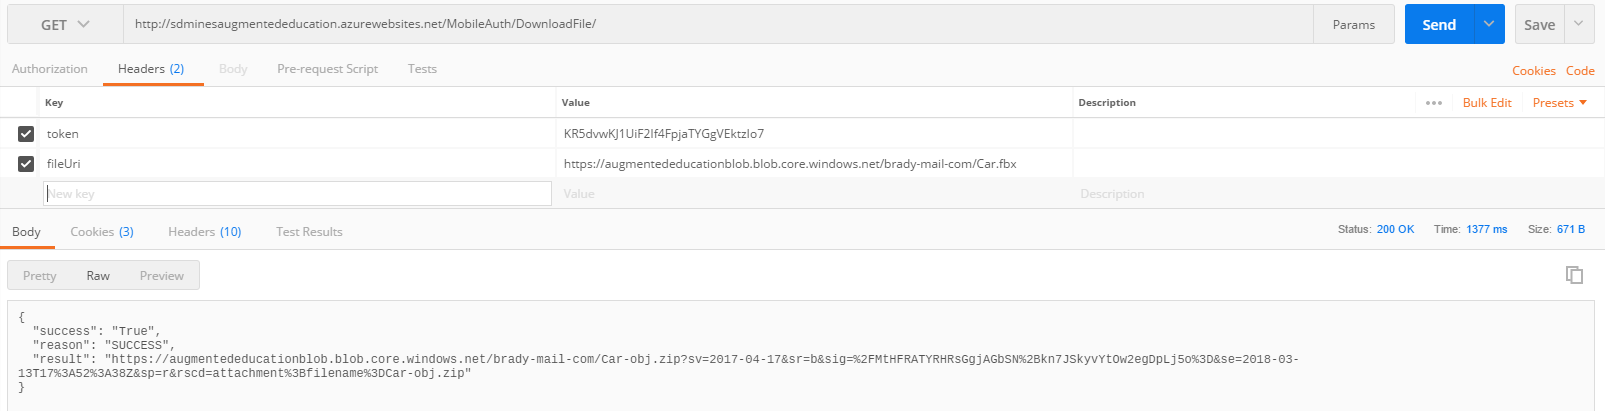
\includegraphics[width=0.75\textwidth]{postman_DownloadFile}
                    \centering
                    \caption{Postman - Download a file}
                    \label{fig:mobilePostmanDownloadFile}
                \end{figure}

                The field \texttt{result} contains the temporary URL.  It would then be put into a web browser (typically Firefox or Chrome) and the file is downloaded.  The file downloaded should be in the OBJ file format, since it is the one that is parse-able by the phone.  The website should use the file conversion software ensure this.  When the models are downloaded, they are stored in a \texttt{Models} directory on the phone.  The file system on the device can be viewed with the Downloads app.  Note, if the model is downloaded, and it does not show up in the file structure, the phone should be restarted.  Commonly, the files do not show up until the device is restarted.  A new folder will be created in the \texttt{Models} directory.  This is because one OBJ model can have multiple other models associated with it, including MTL (material) files and images.  When the models are downloaded, a zip archive is actually downloaded and extracted.

                Future developers should be aware of how the models are saved from the Android download manager.  When making the call for the download manager to do the download, a final path/file name must be provided.  This can cause issues if the file is saved with the wrong extension, especially if the files are viewed on the developers computer (and not just on the phone).
        
        \subsubsection{No Internet}

            Since internet can be less than reliable on cell phones, it was important to test if the there was no internet on the phone.  This was done by turning off Wifi on the testing phones (as they do not have cellular activated).  As expected, if there is no internet, an error message is displayed to the user that the communication was unsuccessful.
        
    \subsection{Offline Mode}
        
        When preparing for the Senior Design Fair, the mobile team decided that it would be a good idea to add an offline mode so the user can view models without having to authenticate with the server.  This was because the Wifi capabilities at the fair would be slim to none.  Therefore, an "Offline Mode" button was added to the login page to allow the user to continue offline.  Testing needed to be done on this to only show models registered as on the phone, as the user would not be able to download remote files without first authenticating.  This was tested and implemented in the application.  The application will not get a list of models from the website or download files from the website in offline mode.  The rest of the functionality (such as viewing the models) remained the same, which was as desired.

    \subsection{QR Code Scanning}
        
        To test that the app was scanning QR codes as expected during development, the team tried a number of different QR codes found online and printed on objects around. There were a surprising amount of these objects on hand with printed QR codes to test with. Testing on these gave an idea of the performance of the QR code scanner for varying QR code sizes.

        The scanner worked with QR codes that pointed to the 3D model downloads.  One difficulty of testing this was the way that the list of models was populated.  When the list was originally populated, all models owned by the user, and models that were public were added to the list.  So, all of the models that the user could access would already be in the list, so scanning a QR code would do nothing.  A later revision changed this so only privately owned files were added to the list, so QR codes can now usefully be scanned. Once the team had the functionality to embed the download link in a QR code, the team tested downloading a number of files manually using their respective QR codes.

    \subsection{Database}
        
        To test the database, the team primarily tested manually by using the test 3D model files. The database is populated by all the models private to the user's account. The team verified that when models are added to the user's account, the database is updated with a listing of the new models. The database also adds entries for scanned QR code files.

% !TEX root = DesignDocument.tex

\section{System Testing}
Testing the system involved manually using the software as a user would.
The test relied on being able to access the website, upload a file, and being able to download the converted version of it.
This was successfully tested through manual tests and these features were present in the MVP.

% !TEX root = DesignDocument.tex

\section{System Integration Testing}

	\subsection{File Conversion and Web}
		
		Manual integration tests were performed while integrating the file conversion software with the website. The integration test was relatively simple and only required the executable to be uploaded to Azure and called as it would regularly be with user requests. Website and file conversion software integration was determined to be complete after multiple successful tests of the complete upload $\rightarrow$ conversion $\rightarrow$ download process.

	\subsection{Mobile and Web}

		Integration between the mobile app and the website takes the form of some endpoints the website will respond to when contacted by the mobile app. The endpoints were developed by the web team; however, the mobile team was consulted for what functionality was required for the app. Members from each group conferred to develop the following endpoints: Authentication, List Models, and Download Models.  As stated in Section \ref{sec:Mobile_Auth}, Postman was used to manually test the endpoints.

		One endpoint that could be created in future developments is the ability to get printable name for a file.  Currently, displaying the name of the file, especially from QR codes, works.  However, the name is very ugly as there is no way to get an easily printable file name.  Scanning a QR code will currently use the URL for the file on the website as the file name in the list. An endpoint for this would allow the phone to better display the models on the mobile device and has been listed as a future development consideration in Ch. \ref{ch:TODO}. 

% !TEX root = DesignDocument.tex

\section{Risk Analysis}
There are two main risks associated with this project. These risks pertain to the functionality of the project itself and the security of its data. Minimizing and preventing these risks are vital to providing quality software and positive relationships with users.

The first risk is that the software may fail to convert or render a given input file. This could be caused by the file being too large, complex, or corrupt for the system to handle. 

In regard to file security, some of the files uploaded may contain sensitive or confidential data. The platform has been designed with the most current security precautions available, but cybersecurity is ever-changing. Security precautions included by the developers may become outdated or deprecated. Additional risk lies in trusting third-party hosting services as these services are frequent targets of cybersecurity threat. 

The project also relies on the Identity and Entity Framework for file access authorization. While this framework is well-respected in the professional development community, it should be noted that the development group is trusting the integrity of the authorization process to this third-party resource.


% !TEX root = DesignDocument.tex

\section{Risk Mitigation}
To mitigate these risks, we have multiple strategies implemented to prevent the issues from happening in the first place.

Addressing the first risk of failed conversion or rendering, we will ensure product quality through rapid iteration and testing of MVPs. 
We have a variety of test files of varying sizes and formats that we have run through our system to make sure we cover many of the common (and uncommon) use cases.
Additionally, we aim to stay informed on the documentation of the libraries and platforms we use in our software to make sure we understand the capabilities and limitations of the tools we are using.
Especially for the file conversion software, we have researched which file types can be run through the libraries and have implemented that functionality in our product and need to communicate to our users which file types are acceptable for our system. 

For the second risk of data security, we try our best to examine and remove any possible security holes in our data flow.
We will need to analyze the website code to limit file access only to properly-privileged users. 
We also plan to implement features such as https and end-to-end encryption to maintain data security on our connections.  %% All tracks
% !TEX root = DesignDocument.tex

\chapter{Sprint Results and Prototypes}    
    \hspace{7mm}This chapter will cover the contents of the tracked sprint progress, as well as any tables, figures, or listings
    pertaining to prototypes througout the development lifecycle.\\

    Sprints are being organized in two-week long segments, starting with sprint 0 being a planning and preparation phase.
    Each sprint detailed in this chapter will consist of:
    \begin{itemize} \item The Backlog \end{itemize}
    
        The backlog of a sprint is to be a list of the items that the development team wishes to accomplish in the duration
        of that sprint. Examples of backlog items could be ``Update documentation for (x)'' or ``Research best practices for (y)''.
        Trivial items, such as fixing a spelling mistake will not be listed on the sprint backlog.\\

    \begin{itemize} \item Successes \end{itemize}
        
        Items from the sprint backlog that were successfully accomplished.  Items listed under the ``Successes'' section
        may contain notes containing specific instructions as to how an issue was resolved.\\

    \begin{itemize} \item Failures \end{itemize}
        
        Items from the sprint backlog that were not successfully accomplished.  Items listed under the ``Failures'' section
        will be accompanied with a description detailing the manner of the failure.  Items to be considered as failed for the
        sprint are backlog items that were not addressed, backlog items that were not fully accomplished, backlog items that
        were attempted to be completed but found to be unreasonable or infeasible (in which case, the requirement needs revision),
        or additional problems that are introduced during the sprint cycle.\\
    \begin{itemize} \item Deliverables \end{itemize}
        
        A description of items from the sprint backlog, more specifically from the ``Successes'' section by the end of the
        sprint cycle, that are considered of value in the hands of the project client.  These are items that validate the 
        continuation of the development process.  Items that are considered to be ``Deliverable'' include, but are not 
        limited to, documentation, wireframes/designs, prototypes, demonstrations, and of course the final product.\\

    \begin{itemize} \item Sprint Review \end{itemize}
       
        An overviewing analysis of the results of the sprint.  This section is where items from the original backlog
        are evaluated and officially labeled as having either passed or failed it's acceptance criteria.\\

        Items having passed their acceptance criteria are appropriately labeled as ``Successes'' for the sprint and are 
        removed from the backlog moving forward to the next sprint development cycle.\\

        Items having failed their acceptance criteria are appropriately labeled as ``Failures'' for the sprint and are
        left on the backlog moving forward to the next sprint development cycle.  The reason for an item being labelled
        as failing for the sprint will be documented and  the item will be re-evaluated to ensure it remains feasible.\\  

    \begin{itemize} \item Sprint Retrospective \end{itemize}
        
        This section will contain both positive and negative remarks from the development team regarding topics such as 
        the rate at which work was completed and the ratio of successes to failures.  Reasons for failing items will be
        discussed and resolutions will be sought after.  If needed, failed items will be re-delegated to one or more 
        developers.\\

        This section also serves as an opportunity for the development team to evaluate the development process as a whole.
        Discussions can be held to suggest changes or improvements to how items are accomplished, or how the development
        process itself is managed.

    \newpage
    % !TEX root = ../../DesignDocument.tex

\section{Sprint 0 Report}
\label{sec:Sprint0_report}
    \subsection{Sprint Backlog}
    \label{sec:Sprint0_backlog}
        \begin{itemize}
            \item Define the toolchain
            \item Define the Minimum Viable Product (MVP)
            \item Create a data flow diagram to detail the MVP            
            \item Identify use cases and create user stories
            \item Estimate a timeline for the development process
        \end{itemize}

    \subsection{Successes}
    \label{sec:Sprint0_successes}
        \begin{itemize} \item Defined the MVP \end{itemize}
        \hspace{7mm}
        Upload a Maplesoft 3D object file to a website.  Have the website perform an automatic file conversion and 
        present the user with an AR Tag.  When the user views the AR Tag through an AR device, download and render 
        the 3D object file.

        \begin{itemize} \item Decided to develop with the Microsoft HoloLens being the primary supported AR device. \end{itemize}
        \hspace{7mm} 
        A conscious decision was made in accordance with current technologies and the Mobile Computing Grant awarded 
        to the South Dakota School of Mines and Technology that this service aims to satisfy to keep development 
        centered around the HoloLens and other Microsoft supported or compatible tools and services.

        \begin{itemize} \item Decided to use Azure for cloud hosting services \end {itemize}
        \hspace{7mm}The decision was between using Azure cloud services or Amazon Web Services. The development team voted to use Azure on the grounds that staying within the Microsoft development network would ensure compatibility with the primary target device, the Microsoft HoloLens, and ease development.

        \begin{itemize} 
            \item Created initial user stories 
            \begin{itemize}
                \item As a faculty member, I want:
                \begin{itemize} 
                    \item to upload a Maple file to a cloud server.
                    \item the Maple file to be automatically converted to an AR tag on the cloud server.
                    \item to be able to download the AR tag for my document from the cloud server.
                \end{itemize}
                \item As a user of this product, I want: 
                \begin{itemize}
                    \item to be able to view the AR tag through a Microsoft HoloLens to render a 3D model.
                \end{itemize}
            \end{itemize}
            \item Estimated tentative development timeline.
        \end{itemize}

    \subsection{Failures}
    \label{sec:Sprint0_failures}
        \begin{itemize} \item None \end{itemize}

    \subsection{Deliverables}
    \label{sec:Sprint0_deliverables}
        \begin{itemize} 
            \item Definition of the MVP
            \item Data flow diagram            
            \item User stories
            \item Defined toolchain
            \item A production timeline (tentative)
        \end{itemize}

    \subsection{Sprint Review}
    \label{sec:Sprint0_review}
        \hspace{7mm}
        All items on the sprint backlog were resolved in a timely, effective manner.

    \subsection{Sprint Retrospective}
    \label{sec:Sprint0_retrospective}
        \hspace{7mm}
        As this is the `setup' sprint, tasks and discussions were primarily limited to topics of planning and preparation.
        The team has been split into two subteams, a web team and a file conversion team.\\ 

        The web team was responsible for the development and management of the ASP.NET website.  This includes the
        structure and design of the website,  as well as the content, account security, organization, and data 
        storage/access.  Members are Daniel Hodgin, Savoy Schuler, and Brady Shimp.\\

        The file conversion team was responsible for research into file type and structure of commonly used 3D modeling
        software such as Maplesoft (TM), and file types that are render-able in commonly used Augmented Reality viewing devices.
        The expected result of the research is to devise a system to convert common 3D modeling software file types into either
        a common file type that is made render-able by commonly used Augmented Reality viewing devices, or a ubiquitous format
        that can then be exported to the necessary file format, depending on which Augmented Reality viewing device is 
        requesting the file. Members are Aaron Alphonsus, Cheldon Coughlen, and Kenneth Petry.
    \newpage
    % !TEX root = ../DesignDocument.tex

\section{Sprint 1 Report}
\label{sec:Sprint1_report}
    \subsection{Sprint Backlog}
    \label{sec:Sprint1_backlog}
    \begin{itemize}
        \item Design website wireframes 
        \item Implement a basic ASP.NET website to mirror wireframes
        \item Be able to upload simple files to the ASP.NET website's web root
        \item Research into widely used and compatible AR renderable file formats
    \end{itemize}

    \subsection{Successes}
    \label{sec:Sprint1_successes}
        \begin{itemize}
            \item Designed website wireframes
                \begin{itemize}
                    \item See figures x - y WARNING - FIX THIS %~\ref{fig:x} - ~\ref{fig:y}
                \end{itemize}
            \item Implemented a basic ASP.NET website to mirror wireframes
                \begin{itemize}
                    \item Hosted on a Microsoft Azure account belonging to Kenneth Petry
                \end{itemize}
            \item Research into widely used and compatible AR renderable file formats
                \begin{itemize}
                    \item Plan:
                        \begin{itemize}
                            \item When a user uploads a file, store it alongside a converted STL format
                            \item Upon access request, convert the STL file to the specified client type
                            \item The converted client type file will be stored with a limited lifetime
                            \item Serve the specified client type file to the user
                        \end{itemize}
                \end{itemize}
        \end{itemize}
    \subsection{Failures}
    \label{sec:Sprint1_failures}
        \begin{itemize} 
            \item Able to upload simple files to the ASP.NET website's web root
        \end{itemize}

    \subsection{Deliverables}
    \label{sec:Sprint1_deliverables}
    \begin{itemize}
        \item Data flow diagrams
            \begin{itemize} \item figures x - y WARNING - FIX THIS \end{itemize} %~\ref{fig:x} - ~\ref{fig:y}
        \item Website wireframe designs
            \begin{itemize} \item figures x - y WARNING - FIX THIS \end{itemize} %~\ref{fig:x} - ~\ref{fig:y}        
        \item A prototype of the website
    \end{itemize}

    \subsection{Sprint Review}
    \label{sec:Sprint1_review}
        \hspace{7mm}
        The only item listed as a failure for this sprint was the ability to upload a simple file
        to the web root folder of the ASP.NET website.  The code had been written by the end of the 
        development sprint cycle, but had yet commited to the repository and therefore was not 
        reviewed and approved.  Testing the functionality of the feature will be one of the primary 
        items in the next sprint development cycle.

    \subsection{Sprint Retrospective}
    \label{sec:Sprint1_retrospective}
        \hspace{7mm}
        The team is in agreement that the sprint went well.  The only item not fully completed was the simple
        file upload, which can be attributed to only one member of the web team working on it while the others
        create early project documents and are being introduced to developing in ASP.NET.  Items of interest 
        during the sprint include the arrival of the Occulus Rift VR headset.  This has sparked discussions of
        supporting hardware.  Future items to consider will be focused around the supplemental hardware needs 
        of the coming AR and VR devices such as:
        \begin{itemize}
            \item What are the minimum hardware specifications for a computer to operate the device?
            \item Where do we get a dedicated development computer with supported hardware?
            \item Where do we store the dedicated computer? 
        \end{itemize}

    \newpage
    % !TEX root = ../../DesignDocument.tex

\section{Sprint 2 Report}
\label{sec:Sprint2_report}
    \subsection{Sprint Backlog}
    \label{sec:Sprint2_backlog}
    \begin{itemize}
        \item Prepare for the first client presentation
        \item Working file conversion in a standalone application
        \item Test that simple file upload to the ASP.NET web root is operable
        \item Define the minimum specifications for a computer to operate pending AR and VR devices
        \item Talk to Professor Schrader about borrowing an old Opp Lab computer for development
        \item Talk to Dr. Rebenitsch about borrowing development work space 
    \end{itemize}

    \subsection{Successes}
    \label{sec:Sprint2_successes}
        \begin{itemize}
            \item Completed the first client presentation
            \item Able to convert file types in a standalone application
            \item Simple file upload to the ASP.NET web root folder is successful
            \item The minimum specifications for a development computer have been defined - ~\autoref{table:metatwosystemrequirements}
        \end{itemize}

    \subsection{Failures}
    \label{sec:Sprint2_failures}
        \begin{itemize}
            \item Unable to borrow development workspace from Dr. Rebenitsch
            \item Professor Schrader has old computers that do not meet the hardware requirements
            \item Professor Schrader is unable to provide us with a development computer that is 
            property of SD Mines without a reserved space  
            \item Textures associated with Maplesoft files are not kept after conversion
            \item The initial proposed software contract presented to SD Mines has been rejected
        \end{itemize}

    \subsection{Deliverables}
    \label{sec:Sprint2_deliverables}
    \begin{itemize}
        \item The first client presentation
        \item Demonstrate that standalone file conversion is operable
        \item Demonstrate that simple files are able to be uploaded to the ASP.NET web root
    \end{itemize}

    \subsection{Sprint Review}
    \label{sec:Sprint2_review}
        \hspace{7mm}
        The proposal to Dr. Rebenitsch to borrow development space in the SD Mines mobile computing lab has
        been rejected so attaining a private development space is still on the backlog moving forward.  Until
        then, Professor Schrader was unable to supply the team with a development computer, so long as the
        computer is property of SD Mines.\\

        Whether a development computer is or is not able to be issued, any of the old Opp Lab computers that Could
        be supplied by Professor Schrader do not meet the minimum hardware specifications for operating AR or VR
        devices.\\

        Through testing the standalone file conversion application, it was learned that Maplesoft files are unable
        to export texture or color properties upon conversion.\\

        The last and potentially largest roadblock encountered throughout this sprint development cycle is the 
        update that the initial software contract proposal that was presented to the Business Office of SD Mines
        has been rejected due to the language in the document specific to 
        \textit{InTouch L.L.C.} 
        retaining intillectual property for the project.  The contact at the SD Mines Business Office is adamant that 
        claims to intillectual property will not be negotiated.

    \subsection{Sprint Retrospective}
    \label{sec:Sprint2_retrospective}
        \hspace{7mm}
        The team is less than satisfied with the result of this sprint but optimistic looking forward.  The
        recorded failing items for this sprint are attributed to outside forces that are not related to the 
        development process.\\

        On the subject of finding a private development workspace, the unanimous decision of the development team is
        that until one is able to be reserved, working sessions involving the AR and VR equipment that is hardware
        dependent will have to be scheduled with a team member who owns a laptop that meets the minimum hardware
        specifications.\\

        On the subject of minimum hardware specifications, the unanimous decision of the development team is that a 
        portion of the project's hardware budget can be set aside for purchasing the necessary upgrades to a computer
        provided by Professor Schrader.  However, the issue of purchasing additional hardware is to be tabled until a
        private development space is able to be reserved.\\

        On the subject of the Maplesoft conversion, research is being done into how to make Maplesoft correctly export
        model color and texture information when the file is converted to an intermediary file type.\\ 

        On the subject of the software contract negotiations with SD Mines, the unanimous decision of the development 
        team is to abandon reliance on the funding from the SD Mines Mobile Computing Grant.  AR hardware will instead 
        be purchased via 
        \textit{InTouch L.L.C.}
        to continue development until completion.  Students shall be compensated as developers following a
        license purchase of the completed product by SD Mines.
    \newpage
    % !TEX root = ../DesignDocument.tex

\section{Sprint 3 Report}
\label{sec:Sprint3_report}
    \subsection{Sprint Backlog}
    \label{sec:Sprint3_backlog}
        \begin{itemize}
            \item Reserve a development workspace
            \item Familiarize with the Microsoft Hololens
            \item Software contract - avoid conflict of interest
            \item Get file conversion operable on the Azure cloud
            \item Research Azure blob storage and similar options for file storage
            \item Be able to download original and converted files the ASP.NET web root
        \end{itemize}

    \subsection{Successes}
    \label{sec:Sprint3_successes}
        \begin{itemize}
            \item Avoid conflict of interest
            \item Familiarize with Microsoft Hololens
            \item Research into Azure blob storage or similar options complete
            \item Able to minimally convert files from type A to type B once on the Azure cloud
            \item Able to download both the original and the converted files from the ASP.NET web root
        \end{itemize}

    \subsection{Failures}
    \label{sec:Sprint3_failures}
        \begin{itemize}
            \item Unable to reserve a development workspace
            \item File conversion on the Azure cloud is not an automatic process
        \end{itemize}

    \subsection{Deliverables}
    \label{sec:Sprint3_deliverables}
        \begin{itemize}
            \item Software contract
            \item Demonstrate that file conversion is operable on the cloud
            \item Demonstrate the basic ability to download documents from the web root folder
        \end{itemize}

    \subsection{Sprint Review}
    \label{sec:Sprint3_review}
        \hspace{7mm}
        A private development workspace is still yet to be reserved.\\

        Conflicts with the SD Mines Buissiness Office have been resolved.  A miscommunication resulted in their
        understanding that the development team intended to be temporarily employed by SD Mines for the duration
        of the 2017-18 academic year to receive funds.  Following policy would then require that all IP be retained
        by SD Mines and not \textit{InTouch L.L.C.}  A problem now arises in that Dr. McGough serves as the PI for
        the SD Mines Mobile Computing Grant and has a percent stake ownership in \textit{InTouch L.L.C.}  Forwarding
        any money from the Mobile Computing Grant to \textit{InTouch L.L.C.} presents itself as a conflict of interest.\\
        
        The Microsoft Hololens arrived and 3D files are able to be tested for AR compatibility.  Upon completing
        the gesture recognition tutorial, it was learned that the Hololens only supports one user account.  To
        change accounts is to factory reset the device and redo setup with a different user account.\\

        The question of file storage space was presented.  Microsoft ImagineX student development accounts do not
        offer space for document storage.  Research was done into the compatibility of Azure blob storage with 
        ImagineX student development accounts and similar options.\\
        
        Files that are uploaded to the ASP.NET web root folder are able to be successfully converted to an alternate
        file format.  Both the original file and the converted file are able to be downloaded from the ASP.NET web root
        folder.  The file conversion process must currently be invoked manually.\\

    \subsection{Sprint Retrospective}
    \label{sec:Sprint3_retrospective}
        \hspace{7mm}
        The team is mostly satisfied with the progress of the sprint.  The only failing items are automatic file
        conversion and reserving a private development workspace.\\

        On the subject of finding a private development workspace, the decision remains unanimous that until one 
        is able to be reserved, working sessions involving the AR and VR equipment that is hardware dependent 
        will have to be scheduled with a team member who owns a laptop that meets the minimum hardware
        specifications.\\

        On the subject of conflicts of interest, the unanimous decision between Dr. McGough and the representatives
        of \textit{InTouch L.L.C.} is that South Dakota Board of Regents policy will be followed to the letter.
        Including a reduced stake in company ownership and leaving decisions regarding purchase orders with the SD 
        Mines Mobile Computing Grant funds up to another SD Mines faculty member who is a signer for the grant.\\
        
        On the subject of Hololens accounts, the unanimous decision of the development team is that a Microsoft
        account will be created and used for the development of this project.  Once development is complete, the 
        device will be reset and returned to SD Mines for configuration.\\

        On the subject of file storage space, options considered were Microsoft OneDrive and Azure blob storage.
        Microsoft OneDrive only allows interfacing via the web from business subscriptions which remain too 
        expensive for the budget of this project and would add a large overhead cost to any future clients.
        Azure blob storage is offered (5 GB per month) for free for a year for a standard trial subscription.
        The unanimous decision of the development team is that when the point in the development process is reached
        where files need to be stored and maintained, the team's Azure subscription will be changed from the 
        ImagineX student developer subscription to the standard free subscription.\\
        
        On the subject of automatic file conversion, it is known that the process needs to be made synchronous
        in order to be automatically invoked when a file is uploaded to the ASP.NET web site.  The item will be
        presented in the backlog of the following sprint.

    \newpage
    % !TEX root = ../DesignDocument.tex

\section{Sprint 4 Report}
\label{sec:Sprint4_report}
    \subsection{Sprint Backlog}
    \label{sec:Sprint4_backlog}
        \begin{itemize}
            \item Generate unique QR codes on a for each uploaded file
            \item Refine development timeline in accordance with the feedback from the client presentation
        \end{itemize}

    \subsection{Successes}
    \label{sec:Sprint4_successes}
        \begin{itemize}
            \item Developed a plan for generating unique QR codes for each uploaded file
            \item Refined the development timeline to postpone multi-user features in lieu of a more basic MVP
        \end{itemize}

    \subsection{Failures}
    \label{sec:Sprint4_failures}
        \begin{itemize}
            \item Unique QR code generation is not yet implemented 
        \end{itemize}

    \subsection{Deliverables}
    \label{sec:Sprint4_deliverables}
    \begin{itemize}
        \item Demonstrate unique QR code generation on a per-file basis
        \item A revision of the development timeline
    \end{itemize}

    \subsection{Sprint Review}
    \label{sec:Sprint4_review}

    \subsection{Sprint Retrospective}
    \label{sec:Sprint4_retrospective}

    \newpage
    % !TEX root = ../../DesignDocument.tex

\section{Sprint 5 Report}
\label{sec:Sprint5_report}
    \subsection{Sprint Backlog}
    \label{sec:Sprint5_backlog}
        \begin{itemize}
            \item Reserve a development workspace
            \item Prepare and give the second client presentation            
            \item Research into Collada file type for Maple textures
            \item Continue work to implement automatic QR code generation
            \item Update project documentation in accordance to the Senior Design Fall 2017 requirements
        \end{itemize}

    \subsection{Successes}
    \label{sec:Sprint5_successes}
        \begin{itemize}
            \item Collada file type research
            \item The second client presentation
            \item Update project documentation for Senior Design
        \end{itemize}

    \subsection{Failures}
    \label{sec:Sprint5_failures}
        \begin{itemize}
            \item Unable to reserve a development workspace
            \item Continue to implement automatic QR code generation
        \end{itemize}

    \subsection{Deliverables}
    \label{sec:Sprint5_deliverables}
        \begin{itemize}
            \item The second client presentation
            \item Project documentation for the 2017 Fall semester
        \end{itemize}

    \subsection{Sprint Review}
    \label{sec:Sprint5_review}
        \hspace{7mm}
        A private development workspace is still yet to be reserved.\\

        Unique QR codes are able to be manually generated given a file path.  A plan exists for automating
        the process but is not yet implemented.\\
        
        Collada file type research shows that the Collada .dae file format should be our intermediary file type.

    \subsection{Sprint Retrospective}
    \label{sec:Sprint5_retrospective}
        \hspace{7mm}
        The development team is in agreement that this was a successful sprint.  The amount of
        content developed during this sprint was minimal in lieu of items such as the client 
        presentation and ensuring the completeness of the documentation required for the 2017
        Fall semester.\\
        
        On the subject of finding a private development workspace, the decision remains unanimous that until one 
        is able to be reserved, working sessions involving the AR and VR equipment that is hardware dependent 
        will have to be scheduled with a team member who owns a laptop that meets the minimum hardware
        specifications.\\

        On the subject of fully implementing QR code generation, the decision remains that 
        the feature is not crucial to the function of the MVP and can be postponed until after the delivery
        of the MVP to be implemented.\\

        On the subject of Collada .dae file type research, The upside of using COLLADA is that it doesn't just 
        contain `geometry data' but also information about motion, light sources, textures etc. COLLADA also 
        has a lot of applications that support it - meaning that being able to export to it and convert it to 
        other formats will probably be easy. The downside to using COLLADA will probably not be an issue. 
        COLLADA has a complex file structure which makes parsing and loading it a challenge. However, at least 
        at this point, it doesn't look like this project will need that. Also, there are a few libraries to 
        help out with this, if needed.\\  %% All tracks
% !TEX encoding = UTF-8 Unicode
% !TEX root = DesignDocument.tex

\chapter{Release -- Setup -- Deployment}

% !TEX encoding = UTF-8 Unicode
% !TEX root = DesignDocument.tex

\section{Website}
\subsection{Considerations}

\tab The following sections covers detailed instructions for publication and deployment of a C\# ASP.NET web application. The publication and deployment steps themselves are relatively simple but there are other factors of the project design that must be taken into consideration before publishing.  

\begin{enumerate}
    \item \textbf{Hosting Environment}

    \tab While ASP.NET Framework web applications are still only supported for production deployments on Windows IIS and Kestrel servers, ASP.NET Core 2+ web applications have been sourced to allow cross-platform production deployment. For this reason, the Visual Studio IDE provides several options for publication targets. These options include:

    \begin{itemize}
        \item Microsoft Azure Virtual Machines
        \item Microsoft Azure App Service -- This is the publication target that is covered later in the document.
        
        \tab The Microsoft Azure related publication targets are for web applications that  runs within the Azure hosted services suite. These methods of publication directly write all new web application source code files to the associated execution directory within the Azure service.  Assuming successful publication, deployment is automatic.
        
        \item IIS, FTP
        
        \tab The IIS, FTP publication target is for directly deploying to the inetpub directory of a Windows Server that the web application developer has credentials and permissions to.  This is similar to the Azure publication target procedure except to a non-Azure Windows Server machine.
        
        \item Folder
        
        \tab The folder publication target is for writing all new web application source code to a local directory on the development machine. This allows more flexibility for custom web application publications.
    \end{itemize}
\end{enumerate}

\subsection{Publication}

\tab The following are steps for web application publication to a Microsoft Azure App Service.\\
    
    \ \\
    \tab $\bullet$ In the Visual Studio IDE, select Build $\rightarrow$ Publish.
    \begin{figure}[H] 
        \centering
        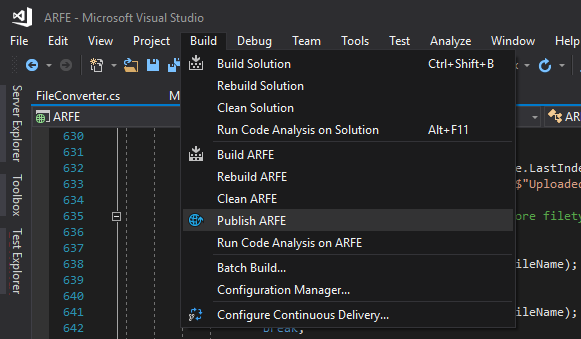
\includegraphics[scale=.6]{select_publish}
    \end{figure}
    
    \ \\
    \tab $\bullet$ If an Azure web application is already created, choose ``Select Existing''.  Otherwise, if there is no web application created, choose ``Create New''.  Choose ``Create Profile''.
    \begin{figure}[H] 
        \centering
        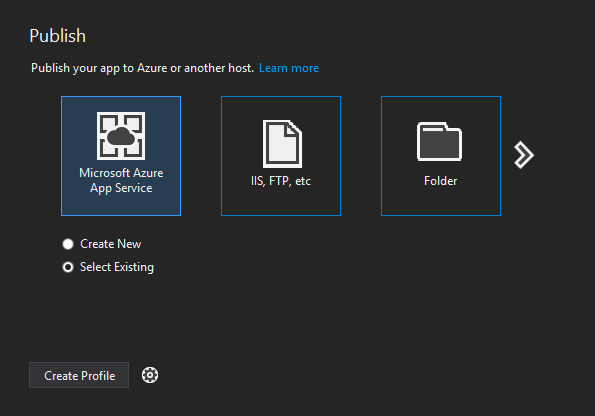
\includegraphics[scale=.6]{select_existing}
    \end{figure}
        
    \ \\
    \tab $\bullet$ This is continuing forward as if the Azure web application is already created. Select the correct web application from the menu of existing applications.
    \begin{figure}[H] 
        \centering
        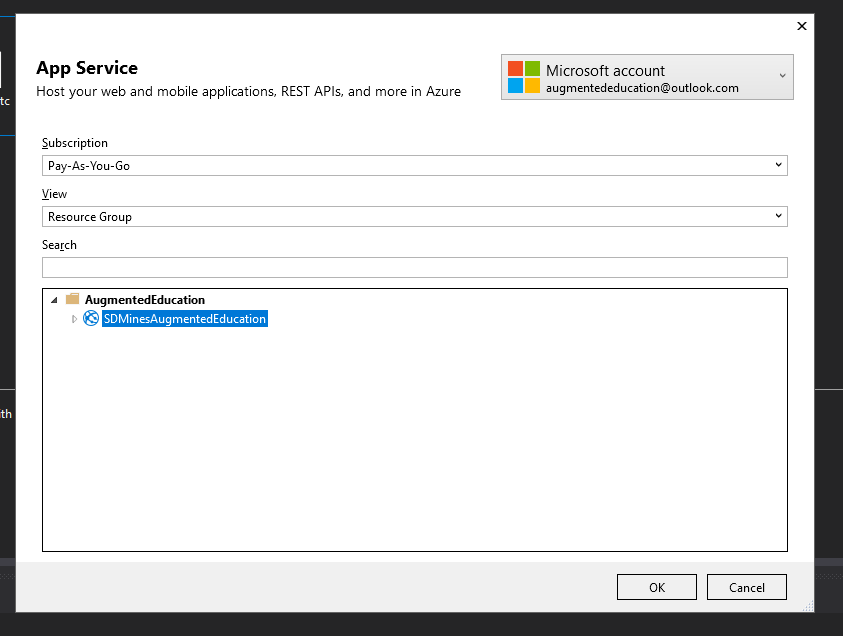
\includegraphics[scale=.6]{select_app_service}
    \end{figure}
        
    \ \\
    \tab $\bullet$ The Summary settings of the selected web application publishing profile should now be shown.
    \begin{figure}[H] 
        \centering
        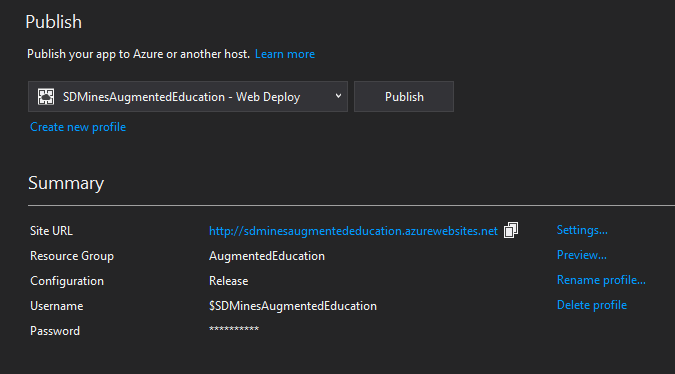
\includegraphics[scale=.6]{review_settings}
    \end{figure}
    
    \ \\
    \tab $\bullet$ Click ``Settings...'' to review the publication profile settings and ensure the fields are filled out similarly as to what is shown.
    \begin{figure}[H] 
        \centering
        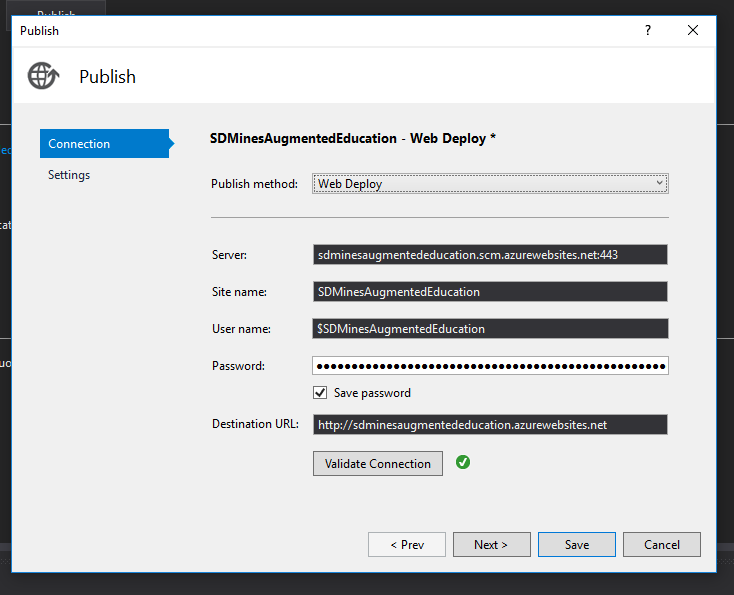
\includegraphics[scale=.6]{connection}
    \end{figure}
    
    \ \\
    \tab $\bullet$ Click ``Next'' to review the configuration settings and ensure the fields are filled out similarly as to what is shown.
    \begin{figure}[H] 
        \centering
        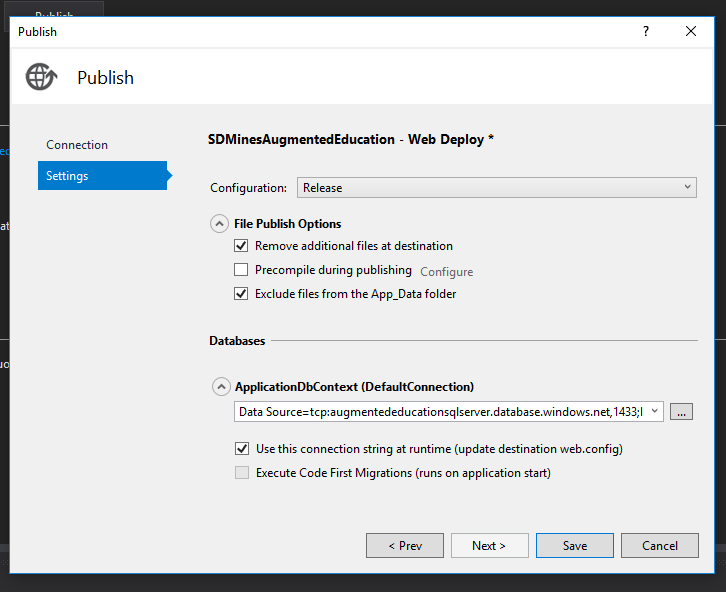
\includegraphics[scale=.6]{settings}
    \end{figure}
    
    \ \\
    \tab $\bullet$ Click ``Save'' on the configuration window and then ``Publish'' on the main Publish screen.
    \begin{figure}[H] 
        \centering
        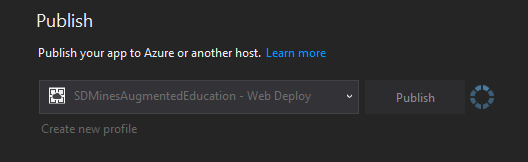
\includegraphics[scale=.6]{publish}
    \end{figure}
    
    \ \\
    \tab $\bullet$ The status of the publication is displayed in the ``Web Publish Activity'' window.  Any publication errors are reported here during the publication process.
    \begin{figure}[H] 
        \centering
        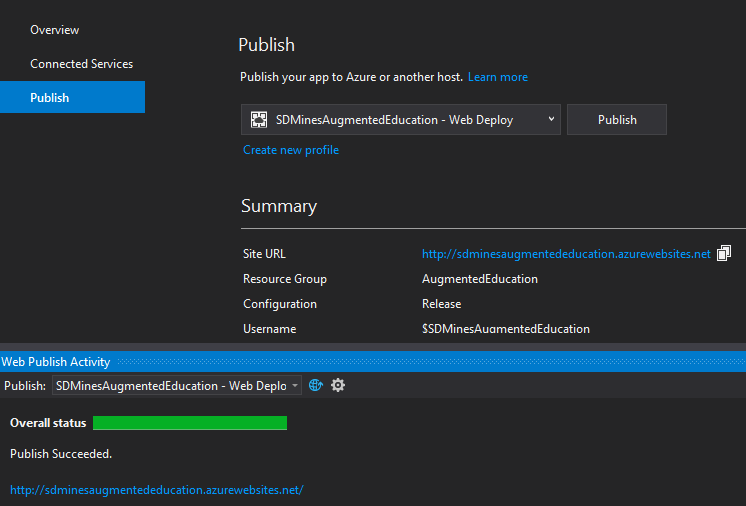
\includegraphics[scale=.6]{publish_succeeded}
    \end{figure}
    \ \\
\subsection{Deployment}
% !TEX encoding = UTF-8 Unicode
% !TEX root = DesignDocument.tex

\section{Mobile}
\subsection{Considerations}
\tab The following sections cover the detailed instructions for publishing an Android App from Android Studio. The first step is to build a "release" version of the app. Once this release app is published, users can install the app through the Google Play Store or directly on their devices. These steps are taken from \url{https://developer.android.com/studio/publish/index.html} where more detailed steps are available for publishing an app.

\subsection{Building Release App}
During development, Android Studio builds the app for "debug" but needs to be modified and rebuilt when it is time to release the app to users.
\subsubsection{Preparing App for Release}
There are multiple steps for preparing an app for release to clean up the code, optimize it, and ensure it is ready for publishing somewhere like the Google Play Store. These steps can be found in more detail at \url{https://developer.android.com/studio/publish/preparing.html}. Some of the major steps are listed below.
\begin{itemize}
    \item Turn off logging and debugging - remove Log calls in code and the android:debuggable attribute from the manifest file.
    \item Clean up project folders - remove unused files and any protected or proprietary files that may have been used in development. This includes assets.
    \item Remove libraries in /lib folder that may no longer be used in the program.
    \item Review manifest and build settings - specify permissions and version numbers and requirements.
    \item Address compatibility issues - different versions of Android and different screen sizes behave differently. Consider using support library to be available to more devices.
\end{itemize}
\subsubsection{Build Release APK}
\begin{itemize}
    \item Build a release APK of the app - in Android Studio under Build -> Build Variant, you want to select "release" to generate a release build to distribute.
    \item Test the release app - install the release build to a development device to ensure that it installs and runs properly.
\end{itemize} 

\subsection{Publishing and Distribution}
There are two main ways to distribute an Android app to users, either by publishing to Google Play or sharing the generated APK file.
\subsubsection{Publishing to Google Play}
There are three essential steps to publishing an app on Google Play, provided in the most up-to-date detail at \url{https://developer.android.com/studio/publish/index.html}. 
\begin{itemize}
    \item Prepare promotional materials - this includes screenshots, graphics, and promotional tet for the Play Store page.
    \item Configuring options and uploading assets - set details such as countries available, price, category, etc.
    \item Publish release version of application - upload the APK built previously to the Play Console and click "Publish" to make it official. Google Play console available at \url{https://developer.android.com/distribute/console/index.html}.
\end{itemize}
\subsubsection{Distributing APK}
Android apps can be distributed through email or websites as well, as long as users can access the APK file on their devices. If the release APK is sent through an email and viewed on the phone, they can tap on the file and it allows them to install it directly. The same process works for downloading the file from a website or loading it into the file system from a computer. Either of these methods require the user to opt-in to installing apps from unknown sources. They need to enable installing unknown apps from their Settings app under Security -> Unknown Sources. After enabling this, they may install the apps directly from an email, website, or downloads app.

\section{File Conversion}

    \subsection{Building}

        Special configurations were set in order to build the project.  There were three places where the configuration was set.  To access the configurations, right click on the \texttt{FileConversion} line, below the \texttt{Solution} line, above all of the source files, and click \texttt{Properties}.  
        
        \begin{enumerate}
            \item Open the \texttt{C/C++} drop-down, select General.  Click on the first line, \texttt{Additional Include Directories}, select the down arrow at the end of the line, and select \texttt{<Edit...>}.  The two configurations are shown in Figure \ref{fig:fileconversionVSConfig1}.  These are the include directories for the libraries.   

            \begin{figure}[H]
                \includegraphics[width=\textwidth]{Deployment/FileConversionVSConfig1}
                \centering
                \caption{File Conversion VS Configuration Include Directories}
                \label{fig:fileconversionVSConfig1}
            \end{figure}

            \item Under the Linker drop-down in the Properties, select General.  Edit the contents of the line labeled \texttt{Additional Library Directories} by clicking on the line, clicking the down arrow at the end of the line, and selecting edit.  The contents of this field are shown in Figure \ref{fig:fileconversionVSConfig2}.  This points the linker to the flies needed for the libraries.

            \begin{figure}[H]
                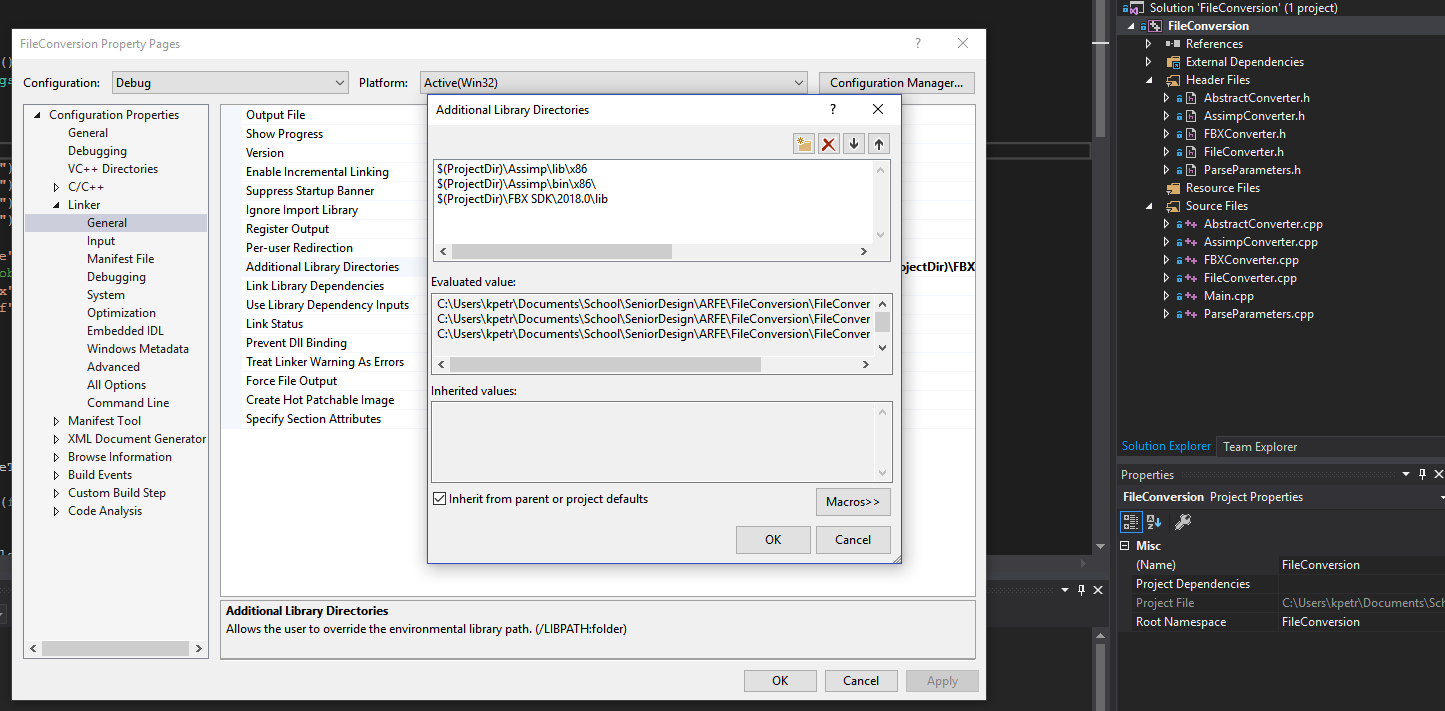
\includegraphics[width=\textwidth]{Deployment/fileConversionVSConfig_Linker}
                \centering
                \caption{File Conversion VS Configuration Linker Configuration - General}
                \label{fig:fileconversionVSConfig2}
            \end{figure}

            \item Under the Linker drop-down in the Properties, select \texttt{Input}.  Edit the content of the first line (labeled \texttt{Additional Dependencies}) by selecting the line, clicking on the down arrow, and clicking edit.  The configuration for this section can be found in Figure \ref{fig:fileconversionVSConfig2}.

            \begin{figure}[H]
                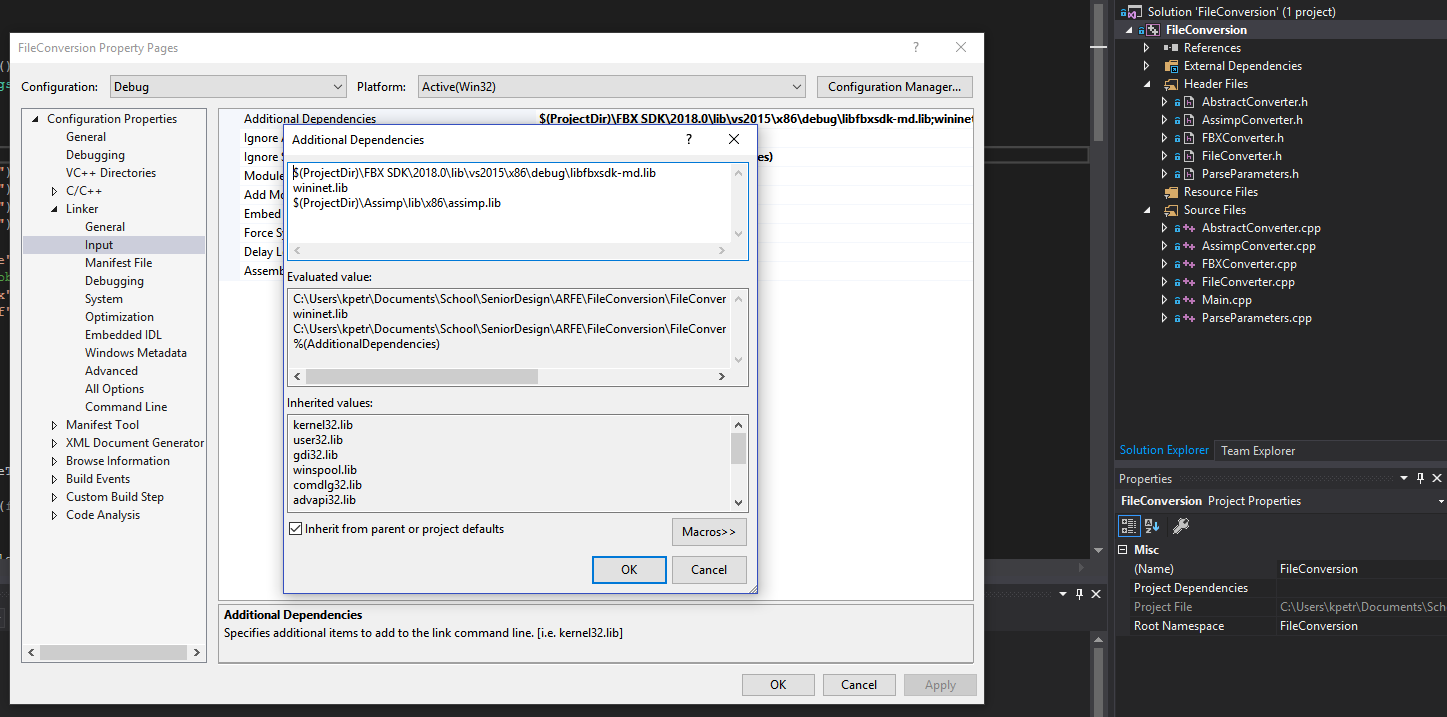
\includegraphics[width=\textwidth]{Deployment/fileConversionVSConfig_Linker_Input}
                \centering
                \caption{File Conversion VS Configuration Linker Configuration - Input}
                \label{fig:fileconversionVSConfig2}
            \end{figure}
    \end{enumerate}

    \subsection{Distribution}

        Two items are needed when distributing the file conversion software: the executable (\texttt{FileConversion.exe}) and a DLL (\texttt{assimp-vc140-mt.dll}).  The DLL is needed for the assimp library for file conversions.

        \subsubsection{Location in the Website}
        The \texttt{FileConversion.exe} along with it's associated (\texttt{assimp-vc140-mt.dll} are located in the ``UploadedFiles" folder under the root web directory (``~/UploadedFiles'').  This directory serves as the root directory for temporary intermediate file storage between the users and Azure Blob Storage.

%This section should contain any specific subsection regarding specifics in releasing, 
%setup, and/or deployment of the system. 
%
%
%\section{Deployment Information and Dependencies}
%Are there dependencies that are not embedded into the system install? 
%
%
%
%\section{Setup Information}
%How is a setup/install built? 
%
%
%
%\section{System  Versioning Information}
%How is the system versioned? 
  %% Normally not research track
% !TEX root = DesignDocument.tex

\chapter{User Documentation}

\section{Overall Guide}
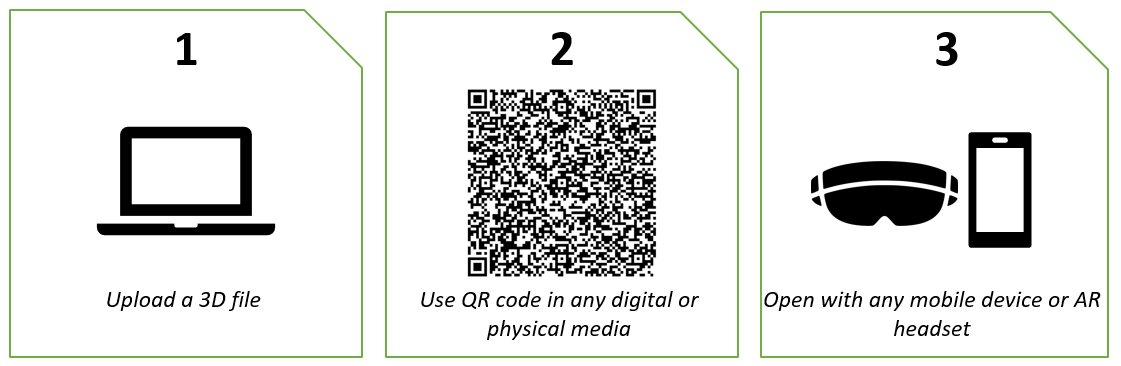
\includegraphics[width=\textwidth]{AugmentedEducationHowTo.png}

\section{User Guide for Website}
\begin{itemize}
    \item Public Content: displays all publicly viewable files.
    \begin{itemize}
        \item Displayed files may be searched or filtered using the Search and Filter bar at the top of the listing.
        \item Clicking a file will reveal options for selecting a file type in which to downloaded the file or for which to a have a linked QR code generated.
        \item QR codes must be generated for mobile devices and all non-mobile devices separately. 
    \end{itemize}
    \item My Content: displays a user's public and private files.
    \begin{itemize}
        \item User's private and public files are displayed in separate tables.  
        \item Tables may be searched or filtered using the Search and Filter bar at the top of the listings.
        \item Clicking a file will reveal options for selecting a file type in which to downloaded the file or for which to a have a linked QR code generated.
        \item QR codes must be generated for mobile devices and all non-mobile devices separately. 
        \item Clicking a file will reveal an options for deleting a file from the cloud. Any QR codes previously associated with the file will no longer work. 
    \end{itemize}
    \item Upload: allows a user to upload a file.
    \begin{enumerate}
        \item Add a file to be uploaded.  
        \item Optionally add a material file to be uploaded. 
        \item Optionally add an alternate display name for the file.
        \item Optionally add a description for the file.
        \item Select whether the file will be public or private.
        \item Press "Upload."
        \item A notification message will appear to indicate success or failure of the upload. 
    \end{enumerate}
    \item Help: displays platform guide for users. 
\end{itemize}

\section{User Guide for HoloLens}
\begin{itemize}
    \item HoloLens Layout

    \begin{figure}[H]
    \includegraphics[width=0.5\textwidth]{HoloLens_Diagram}
    \centering
    \caption{Hololens Layout}
    \label{fig:HoloLens_Diagram}
    \end{figure}

    \begin{itemize}
        \item 1. Power Button
        \item 2. Volume Buttons
        \item 3. Brightness Buttons
        \item 4. Headband Adjuster
        \item 5. Headband
    \end{itemize}

    \item Gestures

    \begin{figure}[H]
        \centering
        
\includegraphics[width=0.25\textwidth]{BloomClose}
        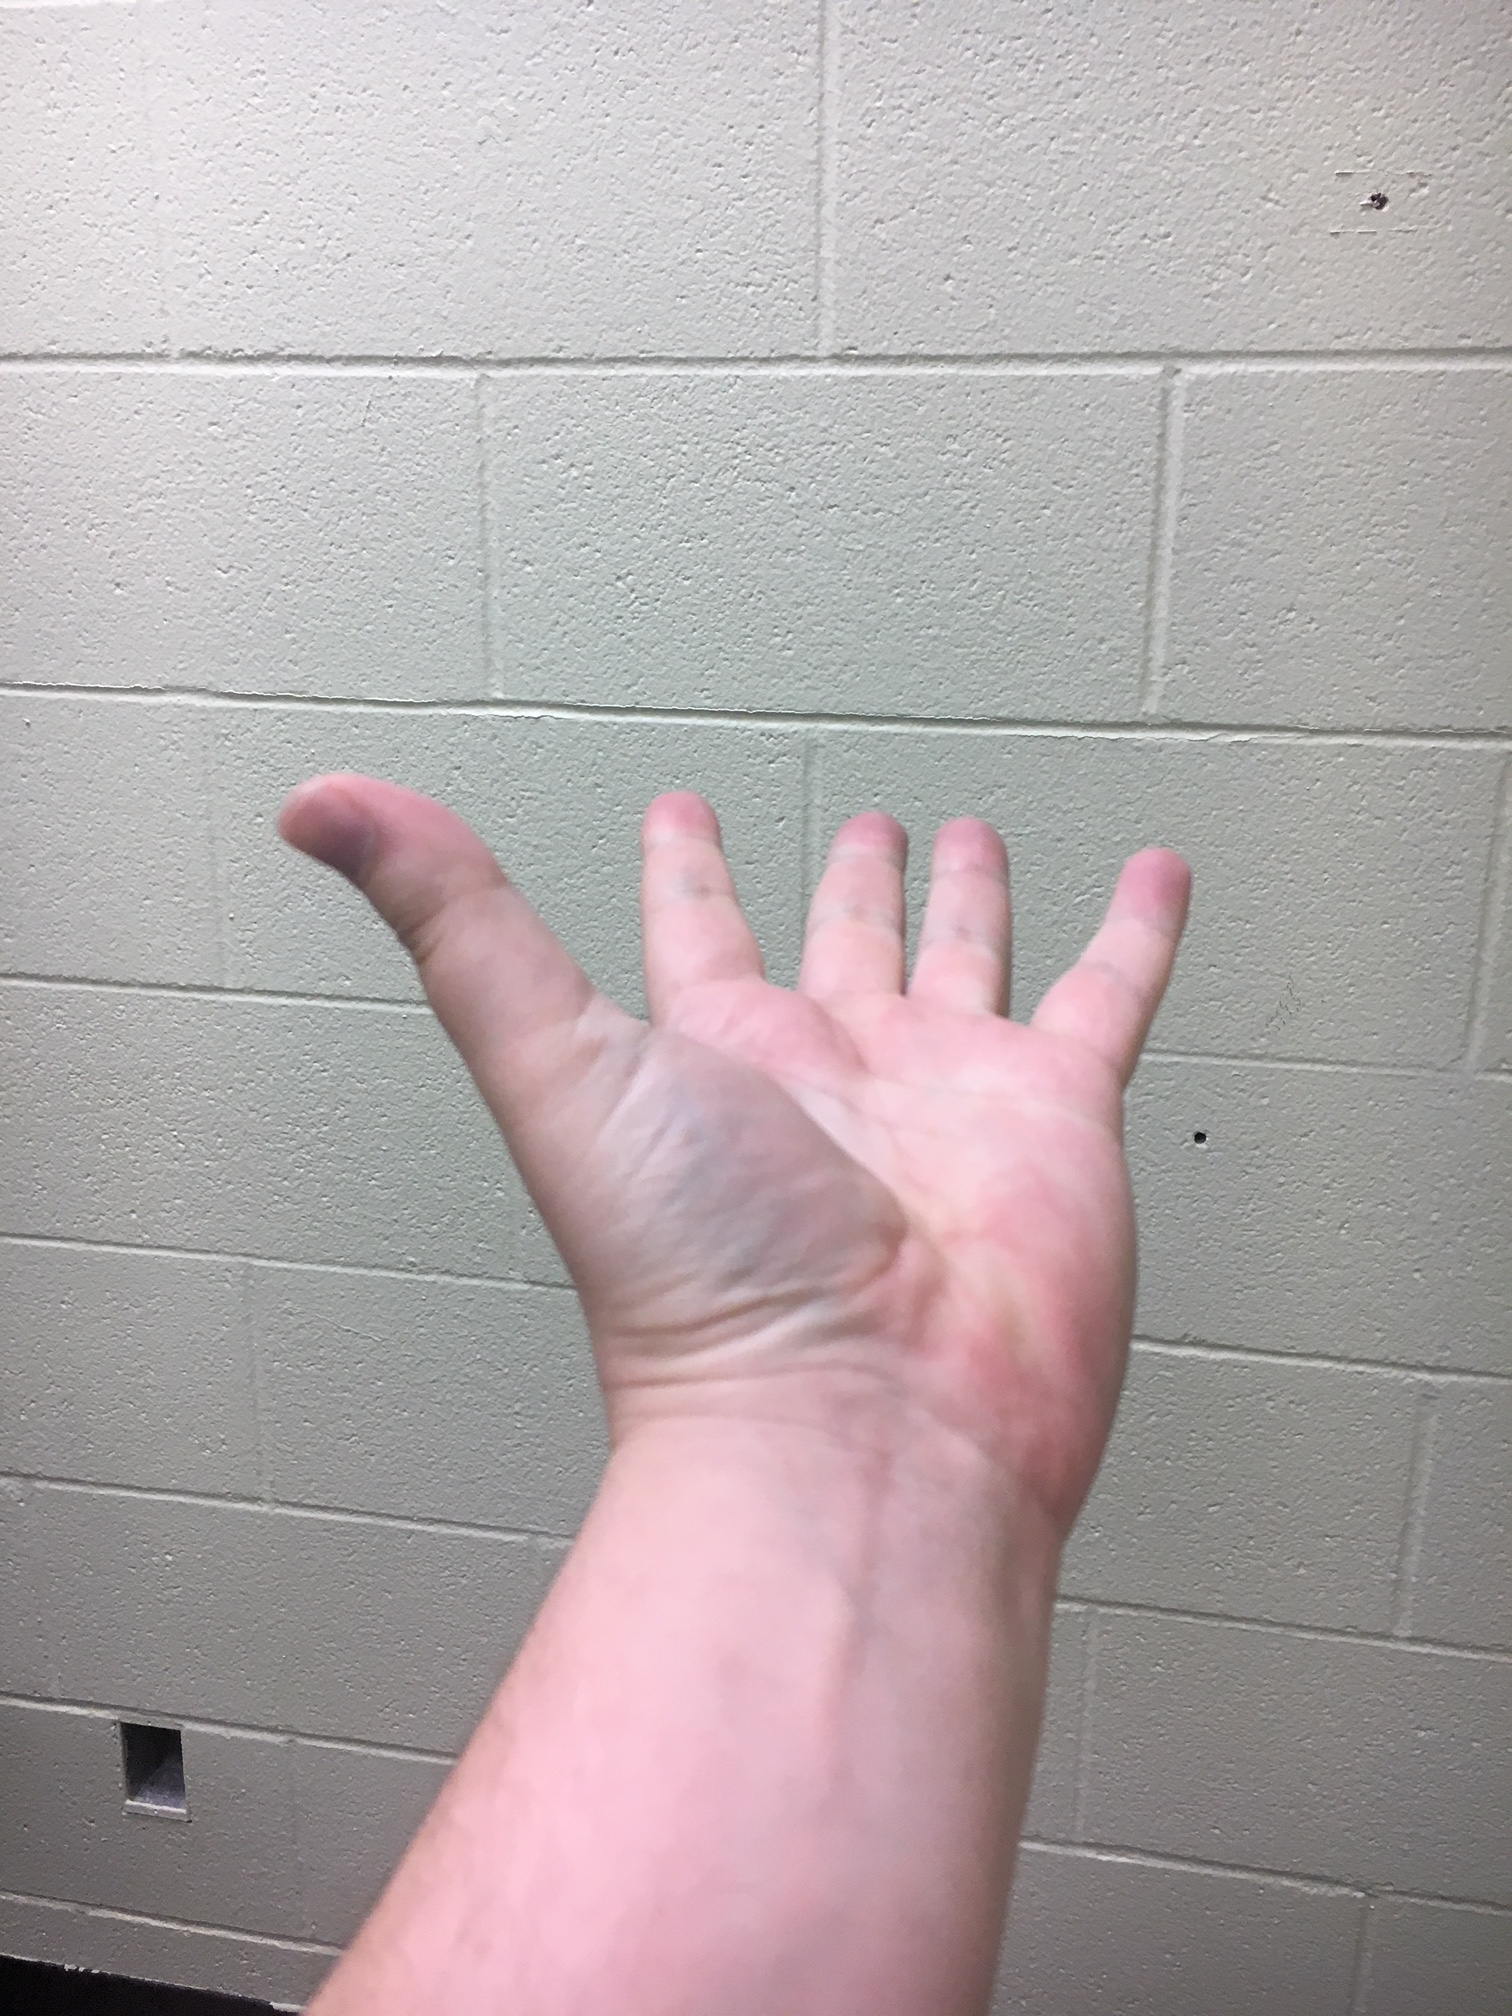
\includegraphics[width=0.25\textwidth]{BloomOpen}
        \caption{Bloom Gesture}
        \label{fig:BloomGesture}
    \end{figure}

        \begin{itemize}
            \item Bloom: Hold out your fist palm up, then open your hand. This is the command to return to the home screen.
        \end{itemize}

    \begin{figure}[H]
        \centering
        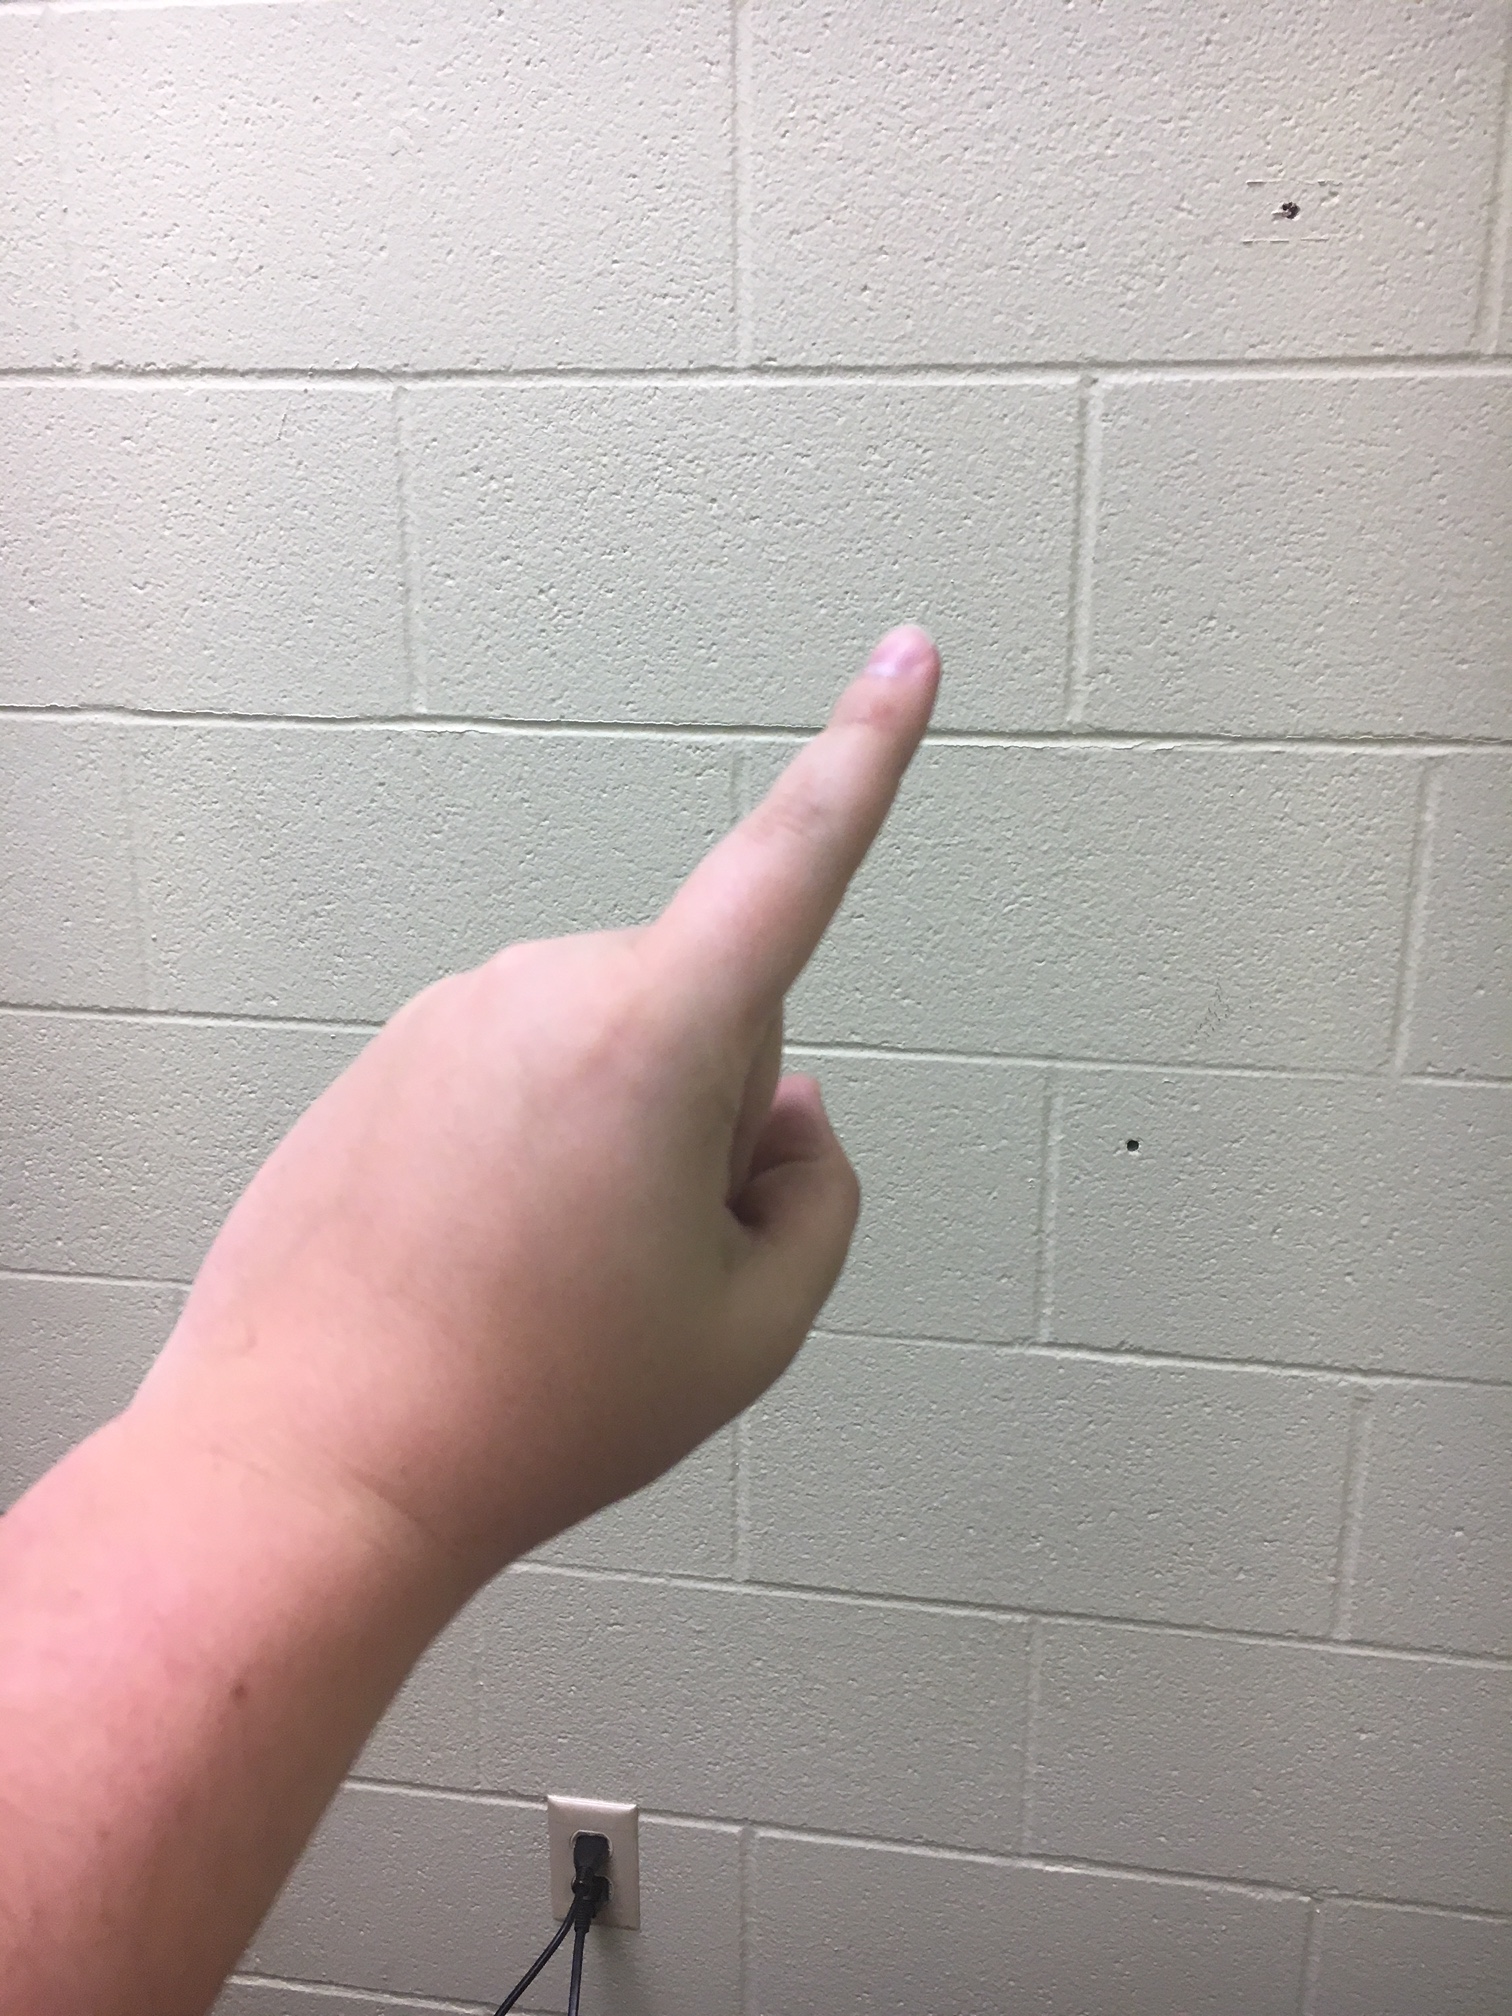
\includegraphics[width=0.25\textwidth]{ClickUp}
        
\includegraphics[width=0.25\textwidth]{ClickDown}
        \caption{Click Gesture}
        \label{fig:ClickGesture}
    \end{figure}

    \begin{itemize}
        \item Click: Hold out your fist with index finger up. Point it down and back up for a single click. Hold the point down for click and hold.
        \item A practice program exist on the HoloLens.
    \end{itemize}

    \item Signing In
        \begin{itemize}
            \item See Dr. Mough for username and password. 

            \item You can type using the HoloLens, but that has proven to difficult. Typing with a computer is made available with the HoloLens App. Details how to connect to that below.
        \end{itemize}

    \item Connecting to the HoloLens App
        \begin{enumerate}
            \item Download Hololens app from the Microsoft Store.
            \item Make sure the HoloLens is in developer mode by enabling it in the system settings
            \item Connect the HoloLens and the computer to the same wifi network.
            \item Connect by inputting the HoloLens IP address. IP address can be found in the network settings.
            \item Login with the Hololens App credentials. See Dr. McGough for login information.
        \end{enumerate}

\end{itemize}

\section{User Guide for Mobile App}
There are four main screens available in the mobile app. These are the login, file listing, QR code reader, and AR view. 
\begin{itemize}
    \item Login Screen
    \begin{itemize}
        \item You may log in using credentials for an account created on the website. Credentials will be saved after the app is closed if you check the box.
        \item Alternatively, you may "Continue Offline" if you don't have a login or don't need to sign in. 
        \item Offline users can view files that are already downloaded on the device and scan new QR codes for adding more models to their list.
    \end{itemize}
    \item File Listing
    \begin{itemize}
        \item The files available to view are listed here.
        \item Some files are already downloaded on the device, and some files are available from the website.
        \item In offline mode, only downloaded files will appear.
        \item A user can select a file from the list. A file that is already downloaded will load in the AR View screen. A file that is not downloaded will be downloaded while a loading spinner appears to demonstrate that the download is in progress.
        \item There is a button available to access the QR Code Reader screen.
    \end{itemize}
    \item QR Code Reader
    \begin{itemize}
        \item The whole screen will be a live feed from the camera.
        \item The user can point their device at a mobile QR code and the app will automatically scan it, returning the user to the File Listing with the new file added.
        \item A user may use the back navigation button to return to the file listing if they choose not to scan a QR code.
    \end{itemize}
    \item AR View
    \begin{itemize}
        \item The AR view allows the user to view the 3D model in their own environment.
        \item The view will have a live feed from the phone's camera.
        \item Small blue points will appear as the phone maps out surfaces.
        \item The user may need to move the device around slowly and allow the phone a few seconds to map flat horizontal surfaces.
        \item When the trigrid appears over the surfaces, the user can tap the screen where they would like to place the model.
        \item After the model is placed, they can use the + and - buttons to change the size, as well as use the number input at the bottom to change how quickly the scale changes.
        \item The user should be able to move around the placed object to see it from different sides, while it remains anchored where it was placed.
        \item If the user covers the camera or turns too far away, the model may lose tracking and need to be replaced.
        \item The user may use the back navigation button to return to the file listing.
    \end{itemize}
\end{itemize}

\section{Demos}

See Appendix \ref{ch:support} for demonstrations of the platform in use. 

\section{User Guide for Capturing Demos}

\subsection{Website}
\begin{itemize}
    \item For screenshots:
    \begin{enumerate}
        \item Navigate to the desired page. 
        \item Find and open Snipping Tool, a default application on windows. 
        \item Select "New" and then select the capture area. 
        \item Save or right-click to copy screenshot. 
    \end{enumerate}
    \item For videos:
    \begin{enumerate}
        \item Open Microsoft PowerPoint.
        \item Navigate to the "Insert" tab. 
        \item Select "Screen Recording." 
        \item Select the recording area.
        \item Press "Record."
        \item To end recording, press the Window's logo key, shift, and "Q" all together.
        \item The recording will now appear in your PowerPoint. 
        \item To save the recording to your desktop, right-click it and select "Save media as..."
    \end{enumerate}
\end{itemize}

\subsection{HoloLens}
\begin{enumerate}
    \item With the HoloLens on, verbally say "Cortana, record this," to begin recording.
    \item Perform the "bloom" motion of opening a closed fist to finish recording.
	\item Recordings will be saved to the One Drive of the account signed in on the HoloLens. Access the One Drive to share and view recordings. 
\end{enumerate}

\subsection{Mobile App}
\begin{enumerate}
    \item Download any screen recording application. 
    \item Open the screen recording application and press the "record" icon.
    \item To finish recording, press the "record" icon again. 
    \item Select "Save."
    \item The video will be saved to the mobile device's gallery and may be shared.
\end{enumerate} %% All tracks
% !TEX root = DesignDocument.tex


\chapter{Research Results}

To be completed Spring 2018.


\section{Hardware}

	% Research / Hardware / ARDevices

\subsubsection{AR Devices}

	Augmented Reality devices are different than VR Devices in that the applications are presented on top of what the user would normally see, not blanking out the screen and recreating the world.  Currently, there are two main headset contenders in the AR space, Microsoft's HoloLens and the Meta 2.  Mobile devices are now becoming more popular for AR.

	\paragraph{HoloLens}

		The HoloLens is a wireless AR headset developed by Microsoft.  The developer edition of the HoloLens was released in March 2016, and has not had any further releases since.  They (Microsoft) are currently developing the HoloLens 2, the next iteration of the hardware.  The origianl version has some user complaints such as a small viewing port, that will be addressed in version two.  

	\paragraph{Meta 2}

		The Meta 2 is another headset.  It is wired, so a computer on par with the requirements for the Oculus VR headset is required.  Being wired is a downside for mobility, in that the user must always be close to a computer.  However, it is also a good thing in that the headset can use the more powerful processing on the computer rather than having the chips on board the headset.

	\paragraph{Mobile Phone}

		AR has recently been moving to the mobile phone space.  Both iOS and Android have AR offerings, ARKit and ARCore respectively.  ARKit was released by Apple in December 2017, and ARCore was released by Google in February 2018.  Since the offerings are so new, the number of applications developed with AR is still limited.  
		
		Mobile devices potentially have a larger consumer base than the dedicated headsets.  Most people have a smart phone (almost all running iOS or Android), and if AR was enabled on those devices, a large portion of the population would have AR capabilities.  Also, the mobile devices are more portable than the dedicated headsets.  A mobile phone can be carried in a pocket or small bag while the headsets must either be worn or be carried in a specialized carrying case.  
		
		One main drawback on running AR through mobile phones is the limited computational power.  A dedicated headset can have specialized hardware (including increased graphics processing) as opposed to a phone.  Also, all of the software on the headsets is designed for AR use.  So the user interfaces are designed with AR in mind, which may or may not be the case for the mobile devices.
	% Research / Hardware / VRAR / VRDevices

\subsubsection{VR Devices}

	Currently (as of May 2018) there are two leading VR headsets: the Oculus Rift and HTC Vive.  The HTC Vive comes in two main forms, the regular Vive and the Vive Pro.  The Vive Pro is a wireless version of the Vive that has better specifications than the regular version.  The Vive sells for around \$500 and the Vive pro for \$800. The Oculus Rift (or Oculus for short) is produced by Facebook and sells for around \$400.

	\paragraph{HTC Vive}

		The HTC Vive is produced by HTC (headquartered in Taiwan).  It is considered the higher tier device (over the Oculus) but also has a higher price tag.  It heavily relies on the SteamVR software produced by Valve.  Tracking for the Vive is done using two "Lighthouses" placed in opposite corners of the room.  They work with the headset and controllers to determine where and what orientation the devices are in.  The information is then sent to the computer and displayed in the application.  The Vive software is heavily integrated with the SteamVR software.  SteamVR is Valve's integration with their popular gaming platform Steam.  It allows users to access their Steam account from within the VR setting to access the store, message friends, and play games.  The connection to the Vive takes place from the headset to a provided "Link box", and from the link box to the computer.  Overall the ports required on the computer are: 1 USB and 1 HDMI.

	\paragraph{Oculus Rift}

		As stated before, the Oculus is produced by Facebook (headquartered in California).  It is a cheaper option compared to the Vive.  It uses its own software to run the headset, but can use SteamVR.  Tracking is performed using two sensors that are placed on either side of the user's computer.  They each take up a USB 2.0 port. Overall, the setup takes 3 USB ports (2x 2.0, 1x 3.0) and 1 HDMI port.

	% Research / Hardware / PC

\subsection{PC}

    Since the school purchased an Oculus and Meta 2, there was a need for a school owned computer that could run them both.  Also, Brent Deschamp was requesting a computer that can run the hardware in order to begin development of content for the website that could be used in his Calculus 3 course.  The most important factor in running the specialized hardware is the Graphics Processing Unit (GPU).  The recommended GPU requirement from Oculus was an NVidia GTX 1060 or above.  

    The original intent at the beginning of the project was to purchase NVidia GTX 1080's (which are better than 1060's).  However, after December of 2017, the price of GPU's increased significantly (in some cases greater than a factor of two).  Therefore, at the time of purchasing the hardware, the price range for the acceptable cards was:

    \begin{itemize}
        \item GTX 1080: \$700 - \$1300
        \item GTX 1070: \$550 - \$700
        \item GTX 1060: \$300 - \$500 
    \end{itemize}

    In order to save the grant money, the original intent of purchasing a 1080 to run the hardware was not pursued.  Instead, an upper tier 1060 was purchased.  The full specifications of the card are listed below:

    \begin{itemize}
        \item ASUS Dual - GTX 1060
        \item 6 GB DDR5 RAM
        \item 2x HDMI Ports
        \item 2x Display Ports
        \item 1x DVI Port
        \item PCIe 3.0 x 16
    \end{itemize}

    In addition to the GPU, a Solid State Drive (SSD) was purchased.  SSD's are like spinning disk hard drives except use flash memory instead of magnetic disks.  They are faster their counterparts, so it decreases boot time and allow for better access during program execution.  The computer that was given to the group to outfit with the GPU only had a spinning disk hard drive, so an SSD was purchased for quality of life improvements while running the hardware.

    Overall the full system specifications for the computer are:

    \begin{itemize}
        \item CPU: Intel i7 ???????
        \item GPU: GTX 1060, 6GB
        \item Storage: 500 GB SSD, 500 GB Hard Disk
        \item RAM: 16 GB
    \end{itemize}

    In order to run the hardware, and develop content for the project, software was needed.  The Oculus and Meta both required software from the hardware manufacturers.  The full list of software initially installed is below:

    \begin{itemize}
        \item Oculus
        \begin{itemize}
            \item Runs the Oculus Rift VR headset.
        \end{itemize}
        \item Meta 2 SDK
        \begin{itemize}
            \item Used to run the Meta 2 AR headset.
            \item Unable to get the software to work due to an error that was occurring during setup.  Error described to Brent on delivery of the computer.
        \end{itemize}
        \item Blender
        \begin{itemize}
            \item Used to visualize some models, including the DAE file type.
        \end{itemize}
        \item Notepad++
        \begin{itemize}
            \item Used to visualize the files on the text level, useful to view/modify OBJ files.
        \end{itemize}
        \item Maple
        \begin{itemize}
            \item Used to generate 3D plots of mathematical functions.
        \end{itemize}
    \end{itemize}

    \subsubsection*{Other GPUs}

        While researching GPU's, the team was asked to research some of NVidia's upper tier GPU's.  The top tier cards are in the Tesla line and are designed for AI research and development.  They do not have any I/O ports, so they are unusable for the devices related to this project.  After research it was suggested that the school seek out a pre-built system that uses the card so there would be a company warranty on the hardware.  This was due to the fact that the cards are very expensive, and a custom built machine has a higher chance of things not working correctly with it, while a pre-built machine would have better integration testing from the manufacturer.
	

\hypertarget{mobile_CodeDocumentation}
{
    \label{mobile_CodeDocumentation}
    \index{mobile_CodeDocumentation@CodeDocumentation}
}

%add section header to first included page
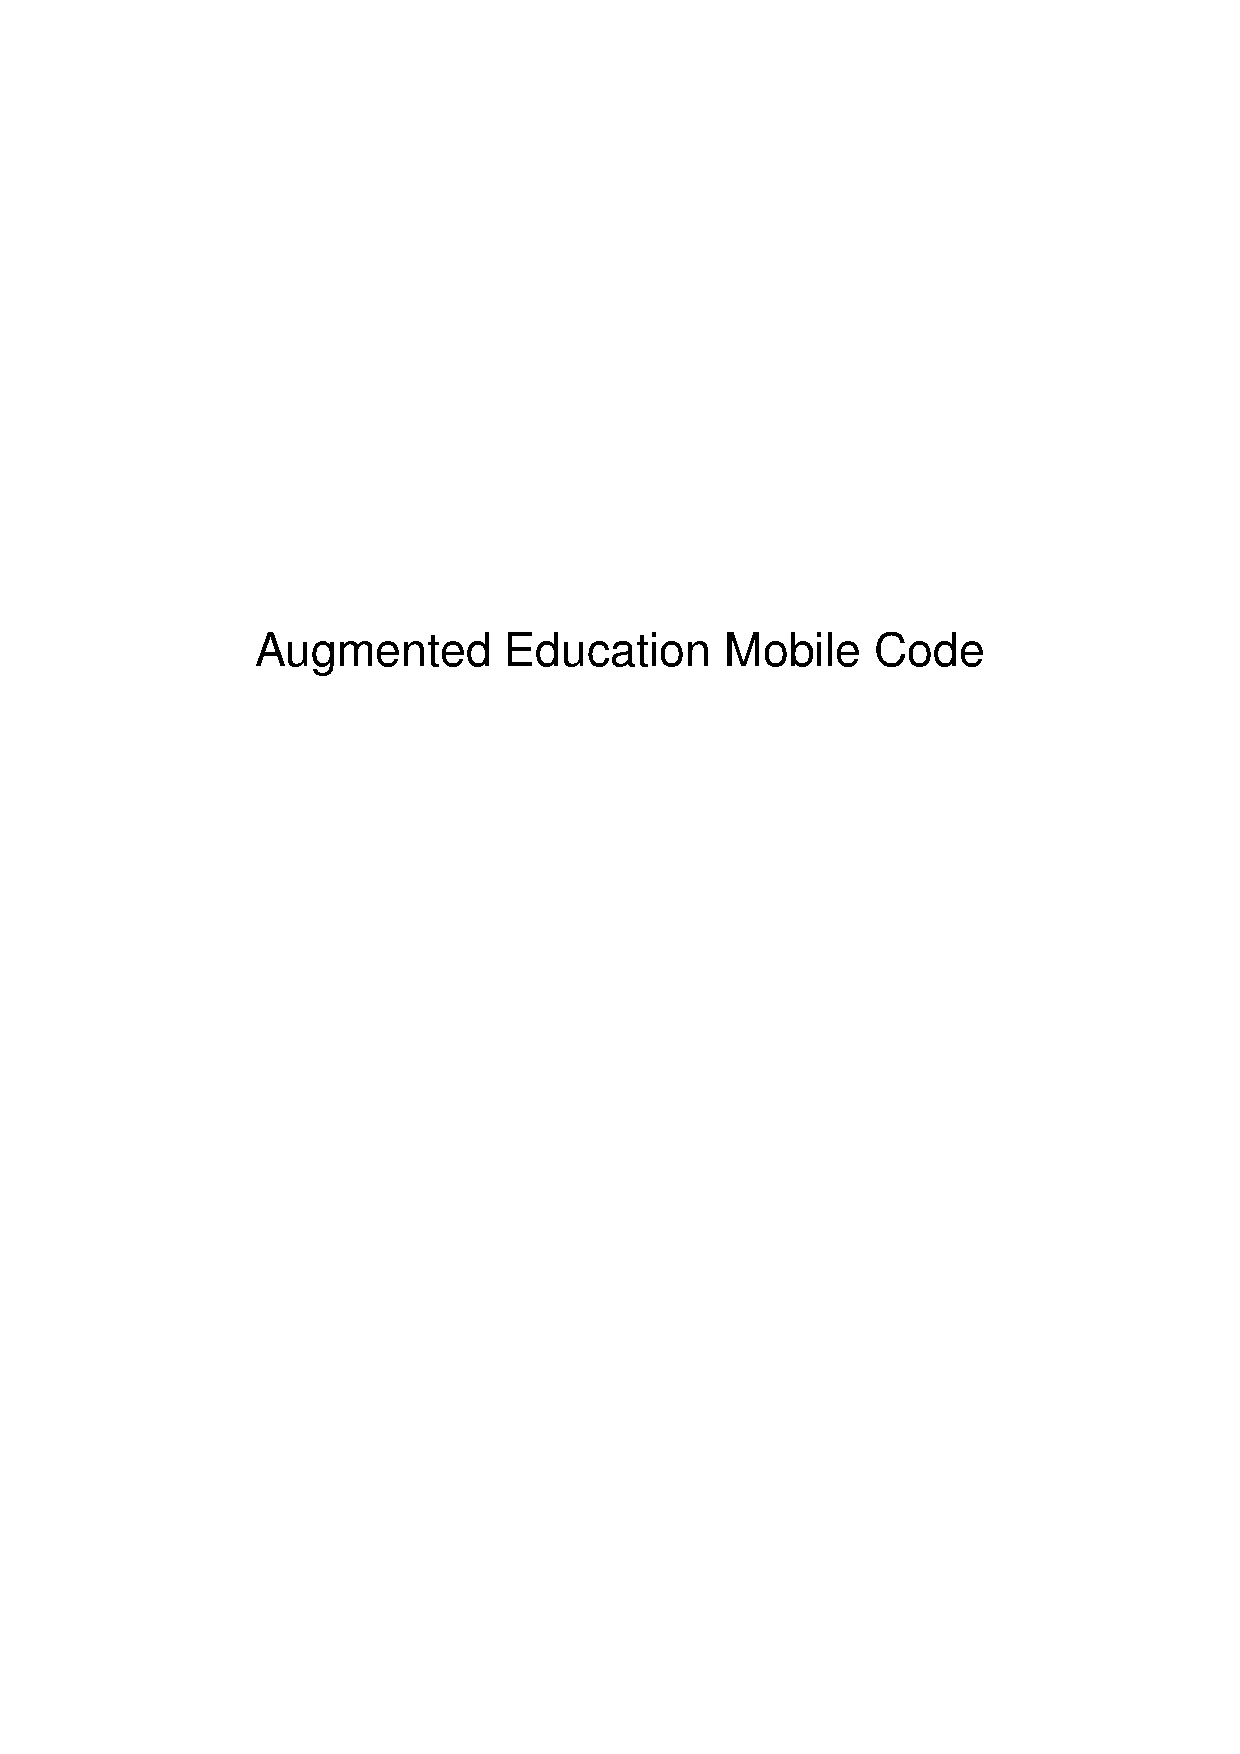
\includepdf[pages={1}, pagecommand=\section{Mobile Application}]{CodeDocumentation/MobileCodeDoc}
\includepdf[pages={2-}]{CodeDocumentation/MobileCodeDoc}

 \section{Website}

 \subsection{Overview}
 \paragraph{}
 The website is a hosting service for uploading, downloading and managing the users files. Microsoft's ASP.NET MVC was used to create the website and Azure was used for its web hosting and file storage tools.
 
 \paragraph{}
 Users can create an account to store and share 3D models with other users. Once a user has an account, they can upload a 3D model as one of the websites supported file types. A user can download the model as any of the supported file types or generate a QR code that can be used for quick download using the mobile app or any other QR code readers.

\subsection{User Interface}
The user interface was designed to be very simple. The UI is comprised of four main pages with a navigation bar to get the pages
    \paragraph{Public Content Page}

        \begin{figure}[H]
        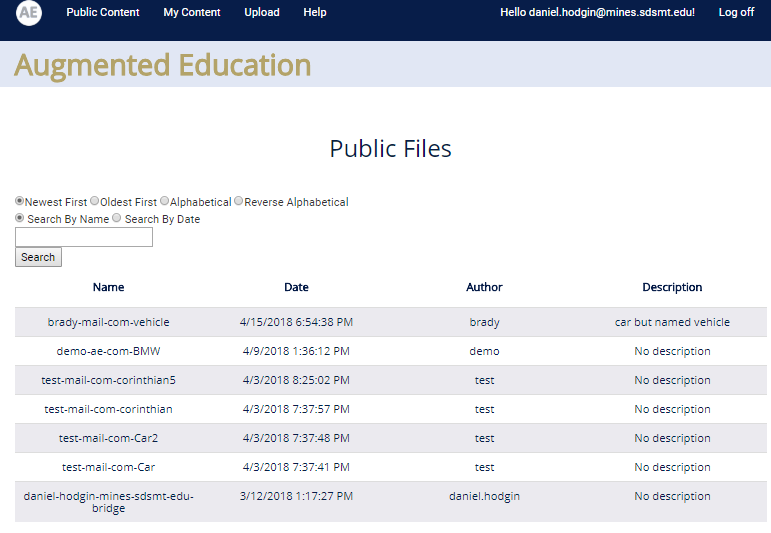
\includegraphics[width=0.5\textwidth]{Web/PublicPage}
        \centering
        \caption{Public Content Page}
        \label{fig:PublicContent}
        \end{figure}

        This is the main landing page for the website. From here users are able to browse the public files to download and generate QR code. Users do not need to be signed in or have an account to access the information on this page.

    \paragraph{My Content Page}
        \begin{figure}[H]
        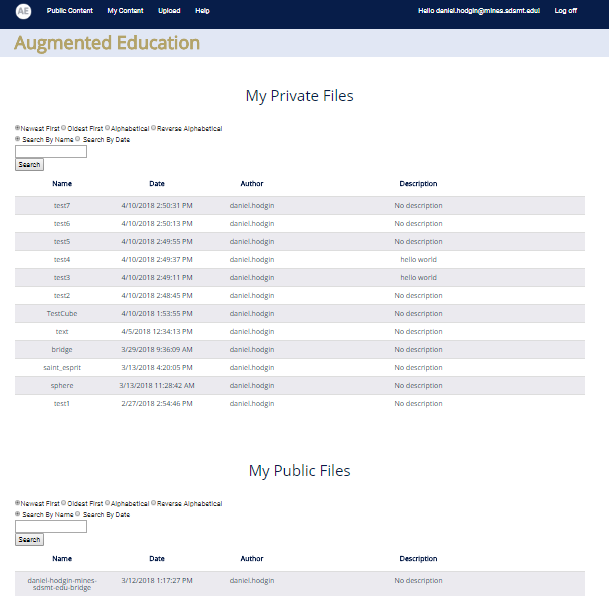
\includegraphics[width=0.5\textwidth]{Web/MyContent}
        \centering
        \caption{My Content Page}
        \label{fig:MyContent}
        \end{figure}

        This page will display all of the content that a user has uploaded. Here a user can browse their private and public files to download and generate QR codes. Users also have the ability to delete files. Users must have an account to access this page.

    \paragraph{Upload Page}
        \begin{figure}[H]
        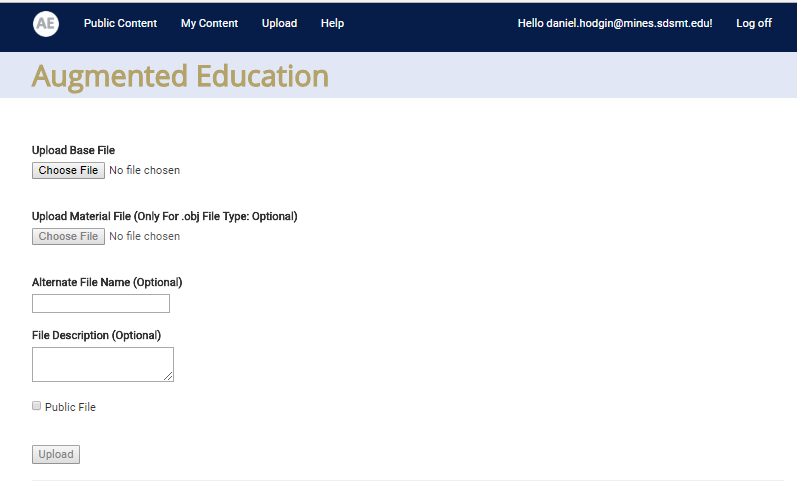
\includegraphics[width=0.5\textwidth]{Web/Upload}
        \centering
        \caption{Upload Page}
        \label{fig:UploadPage}
        \end{figure}

        This page will allow users to upload 3D models. Users can upload a material file if it is an OBJ file. The user can add a description, specify an alternate name, and make the file public. Users must have an account and be signed in to access this page.

    \paragraph{Help Page}
        \begin{figure}[H]
        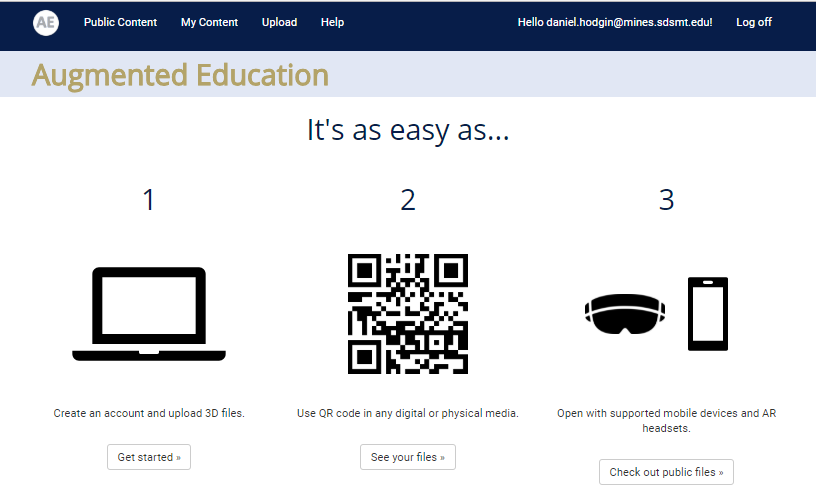
\includegraphics[width=0.5\textwidth]{Web/Help}
        \centering
        \caption{Upload Page}
        \label{fig:HelpPage}
        \end{figure}
    
        This page just gives a simple tutorial on how to uses the website.

\subsection{Technologies Used}

    As stated earlier in this document, this product is making use
    of the Microsoft environment for its tools. Below is an in-depth 
    breakdown of the tools currently being used:

    \begin{itemize}
    \item ASP.NET MVC
    \begin{itemize}
        \item An MVC web architecture, where the backend logic is written in controller classes
        that send and receive data from the client.
        \item It allows for dynamic html pages using a Razor syntax. Razor allows
        you to embed C\# Code into the html and execute logic.
    \end{itemize}
    
    \item Azure
        \begin{itemize}
            \item Microsoft cloud hosting services.
            \item Allows for simple database and web hosting.
            \item Paid features are offered free to students.
        \end{itemize}
    \end{itemize}

    These tools make up the core development of this website. The website is also
    making use of other smaller packages to handles user authentication and database management.

    The website also implements the file conversion software that is described later.
    The file conversion was written in C++, so it couldn't be compiled with the website.
    The workaround was that the file conversion was compiled into an executable that can be used through a system command to convert the file.


    \subsection{Data Flow}
    The website acts as an intermediary between the user and the cloud. Data flow for the website can be broken into a upload and download data flow.

    \paragraph{Upload Data Flow}
    \begin{itemize}
        \item Once a user upload a file it is temporarily save on the server.
        \item If the file is not a FBX file it is converted to a FBX file.
        \item The file is then uploaded to Azure blob storage for long term storage.
        \item The file on the server is then deleted on a sucessful upload to Azure.
    \end{itemize}

    \paragraph{Download Data Flow}
    \begin{itemize}
        \item When a user requests to download a file or generate a QR code, the file name and type is sent to the server.
        \item The server pulls the file from Azure and temporarily save it to the server.
        \item If a download is requested, it does a conversion if nessessary and send the file to the user.
        \item If a QR code is generated, it does a conversion if nessessary and then saves it back to Azure storage and returns a link to the file in Azure embedded in a QR code.
        \item 
    \end{itemize}


\subsection{Design Details}

    \subsubsection{Overview}

    The website was written in C\# with the ASP.NET MVC framework. The main logic
    of the website are contained in two controllers
    \begin{itemize}
        \item Upload Controller
        \begin{itemize}
            \item Handles upload from client to the server.
            \item Uses File Conversion executable to convert to .fbx
            \item Stores file on the web.
        \end{itemize}
        \item Download
        \begin{itemize}
            \item Uploads Model tag from client to server.
            \item Finds associated store model.
            \item Returns model to the client.
        \end{itemize}
    \end{itemize}

    \subsubsection{Code Structure}
    As stated before the website is using ASP.NET MVC framework. 
    The logic happens in the controllers and is split up into the upload and download controller.
    
    \paragraph{Parameter Passing}
    \hfill \break
    The main functions that are being used are the upload and download function.
    
    \begin{itemize}
        \item Upload Function
        \begin{itemize}
           \item HttpPostedFileBase - http message sent from client to server containing the file
           \item The message is parsed to retrieve the file and save to the web.
        \end{itemize}

        \item Download Function
        \begin{itemize}
            \item input string ModelTag - string containing the reference tag to the model.
            \item output httpresponse - http message sent from server to client containing the file. 
        \end{itemize}
    \end{itemize}

\section{File Conversion}

    An early section of the research in the project was on file conversion.  The goal was to make some software that takes in a wide variety of 3D model file types and export them to file types that would be viewable on VR/AR devices.  This section outlines the specifics of what the research found.

    \subsection{File Types}

        There are a large number of available 3D model file types.  However, a small subset of those file types are supported on most devices.  These include the .fbx, .dae, and .obj file types.  Of the three, the .obj is the simplest to understand and modify, since it is stored in large plain text lists.  The others are more complicated, and research on how the files are actually structured was not pursued.

        \subsubsection{FBX}

            The FBX file type is provided by AutoDesk.  It is heavily supported on the HoloLens, where the default viewer can open and display the file easily.  Files stored as this type are commonly smaller than the same file stored as other types.

        \subsubsection{DAE}

            The DAE file type, also called Collada, is used as a common intermediary type in our project.  The only widly available software that can open and dispaly .dae files is Blender.  However, it is not common for people to have Blender installed.  If the user had not used the software before, there is a steep learning curve, so it is not recommended that users use this as the final file type.

        \subsubsection{OBJ}

            The Wavefront OBJ file type is a standard format supported by almost all viewers.  It is simple to understand, but it structure leads to a very large file size.  Also, any materials in the file are stored in separate files, so multiple files must be managed in order to view a model.  Therefore, this file type is a poor choice for a common interchange due to the large size and complexity.

            \paragraph{Structure}

                The file structure of OBJ files is very easy to understand.  For a more in-depth understanding, the Wikipedia page on the file type gives a very good description (\url{https://en.wikipedia.org/wiki/Wavefront_.obj_file}).  A brief synopsis is given below.

                The main file (<filename>.obj) contains the body of the model, and any additional files are materials.  The material file have a .mtl extension (or appropriate image file extensions for embedded images).  The obj file itself contains a large list of vertices given as Cartesian coordinates in 3-space.  Other lists such as texture coordinates, normal vectors, and parameter space vertices are listed.  The other important list is the list of faces.  A face is defined by a set of interconnected vertices.  A material in the .mtl file can be specified before listing faces to set the currently active material.

            \paragraph{Embedded Images}

                Image files (such as .png or .jpeg) can be embedded in the model.  They are defined in the .mtl file when declaring a material.  When the model is parsed and drawn, the images must be located.  One issue found on this topic is the file paths to the images.  In most models tested, the path is an absolute path.  Therefore, when the user uploads or moves the file off of their computer, the image path may be inaccurate and the viewing software may have a rough time when displaying the model.

        \subsubsection{Exporting from Common Programs}

            \paragraph{Maple}

                One of the user stories required the need to export the 3D model from the Maple software used by the math department.  The following statement can be used to export a \texttt{plot3d} plot from Maple into an obj file type:

                \noindent\makebox[\linewidth]{\rule{\textwidth}{0.4pt}}

                \begin{figure}[H]
                    \verbatiminput{Graphics/MapleText.txt}
                    \caption{Maple code to export \texttt{plot3d()} plot}
                \end{figure}

                \noindent\makebox[\linewidth]{\rule{\textwidth}{0.4pt}}                

                The tested, common file types Maple can export are: OBJ, DAE, PLY.  Note that Maple cannot export FBX files (tested in Maple 18, May 2018).  To change the name of the file, change the text \texttt{test1.obj} to the desired file name and extension.  If the file extension is not supported by Maple, a warning message is printed instead of actually producing the file.  Currently, the code exports the model to the same location of where the Maple file is saved.  The save directory can be specified by replacing the text \texttt{currentdir()}.  The desired equation must be written in the \texttt{plot3d()} function as per Maple syntax.  As a note, as of May 2018, Maple does not export textures/colors, so the models default to white.

            \paragraph{Solid Works}
                
            The Solid Works documentation stated that it could export to the desired 3D file types.

    \subsection{Libraries}

        The two libraries used for file conversion were heavily discussed in previous sections.  Therefore, a brief summary of what occurs is described here.

        The Open Asset Import Library (assimp) supports importing and exporting to a wide variety of file types.  However, it has issues when working with the fbx file type.  Therefore, the FBX SDK from AutoDesk is used to handle the conversion to and from fbx files.  If neither library can complete the conversion on its own, then both libraries are used to do the conversion.  In this case, one library creates a .dae file that is consumed by the other library.  This allows for the two libraries to work together and convert to almost any file type desired.

    \subsection{Implementation and Uses}

        This section covers how the file conversion research and software is applied in the project.  This mostly includes the use cases for the file conversion software that was developed.

        The website is the main consumer for the file conversion software.  It is the entity that makes a call to convert a file to a different type.  The goal was to abstract the file conversion away from the user so they do not need to worry about different types and what works, and what does not.  
            
        A call to the file conversion is performed whenever a user uploads a file.  It converts the uploaded file into the .fbx type for storage.  Then, the user can request a download through the website to different file types.  This calls the file conversion software.  Also, if a request comes in through the Rest API (typically through mobile), a file conversion may take place.  A mobile device makes a request for the obj type, as it is what can currently be rendered.


\section{Mobile Testing}
    Testing for the mobile app was primarily done manually. This is because most testing was done on visualizing files and verifying the app performed as expected.  It was also verifying that HTTP packets were as expected going to and from the phone.

    When error messages are printed to the user of the app, a toast is displayed.  A toast is the small box that pops up on the lower section of the screen.

    \subsection{Files}
        A variety of files were used throughout development to test functionality of the app. Some sample files were found on \url{https://free3d.com}. Some files were provided from Dr. Deschamp and others were generated in Maple. Different files were used to test that colors were working both in the MTL and as PNGs. Additionally, large and small files were tested to see how the app reacted to more complex files. The BMW file seen below is an example of a complex file that doesn't render well in the app and demonstrates the limitations of the app.
        
        \subsubsection{Colors}
        
            A major feature requested for the app was to be able to display colors. The example below shows a simple sphere with a proof of concept that colors do work. The car is a more in-depth example that shows multiple colors on the same model.
            
            \begin{figure}[H]
                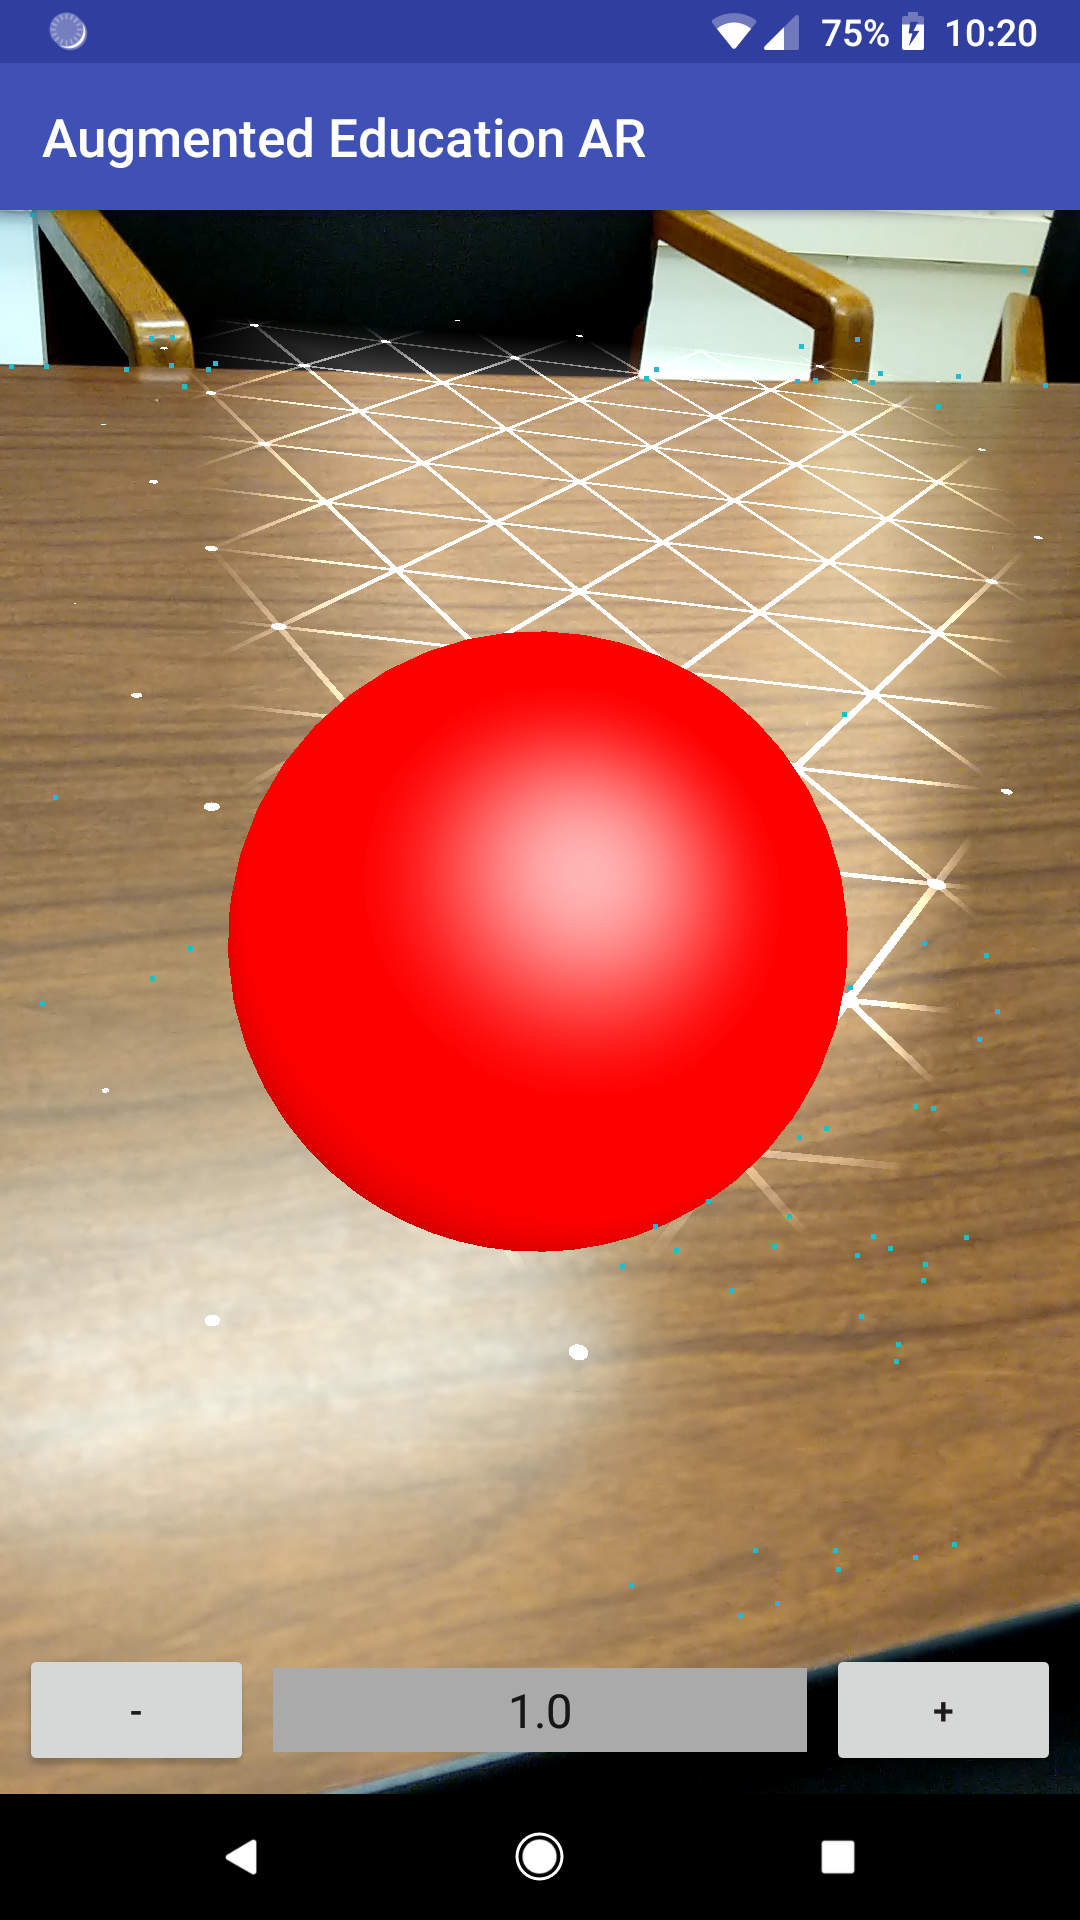
\includegraphics[width=0.5\textwidth]{Mobile/Mobile_RedSphere}
                \centering
                \caption{Colors - Red Sphere}
                \label{fig:mobileRedSphere}
            \end{figure}

            \begin{figure}[H]
                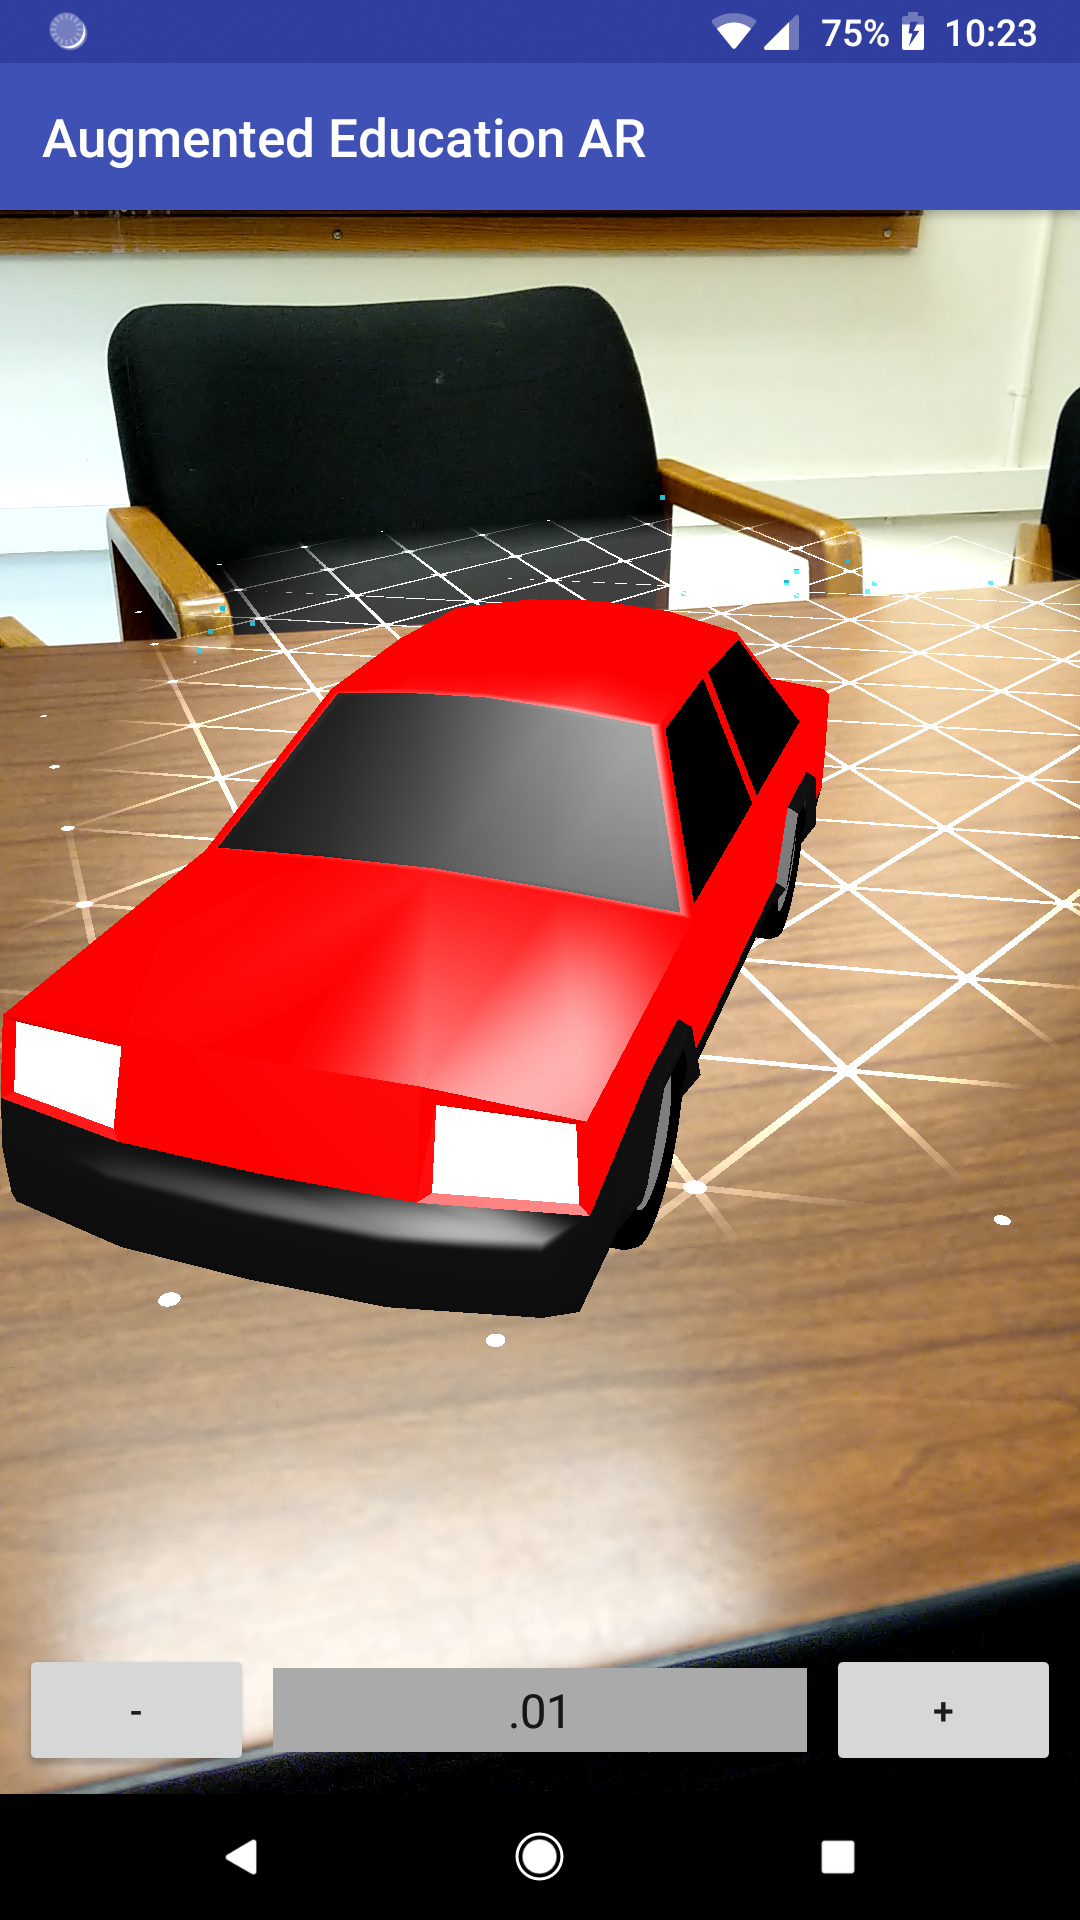
\includegraphics[width=0.5\textwidth]{Mobile/Mobile_Car}
                \centering
                \caption{Colors - Car}
                \label{fig:mobileCar}
            \end{figure}
        
        \subsubsection{Large Files}
        
            One main concern was that 3D files can get large and complex. The BMW is an example of this because it has 51,318 vertices while the sphere only has 2,258. It took a longer amount of time ($\sim$5 seconds) to load this file and it draws poorly, showing a limitation of keeping track of so many vertices.
            \begin{figure}[H]
                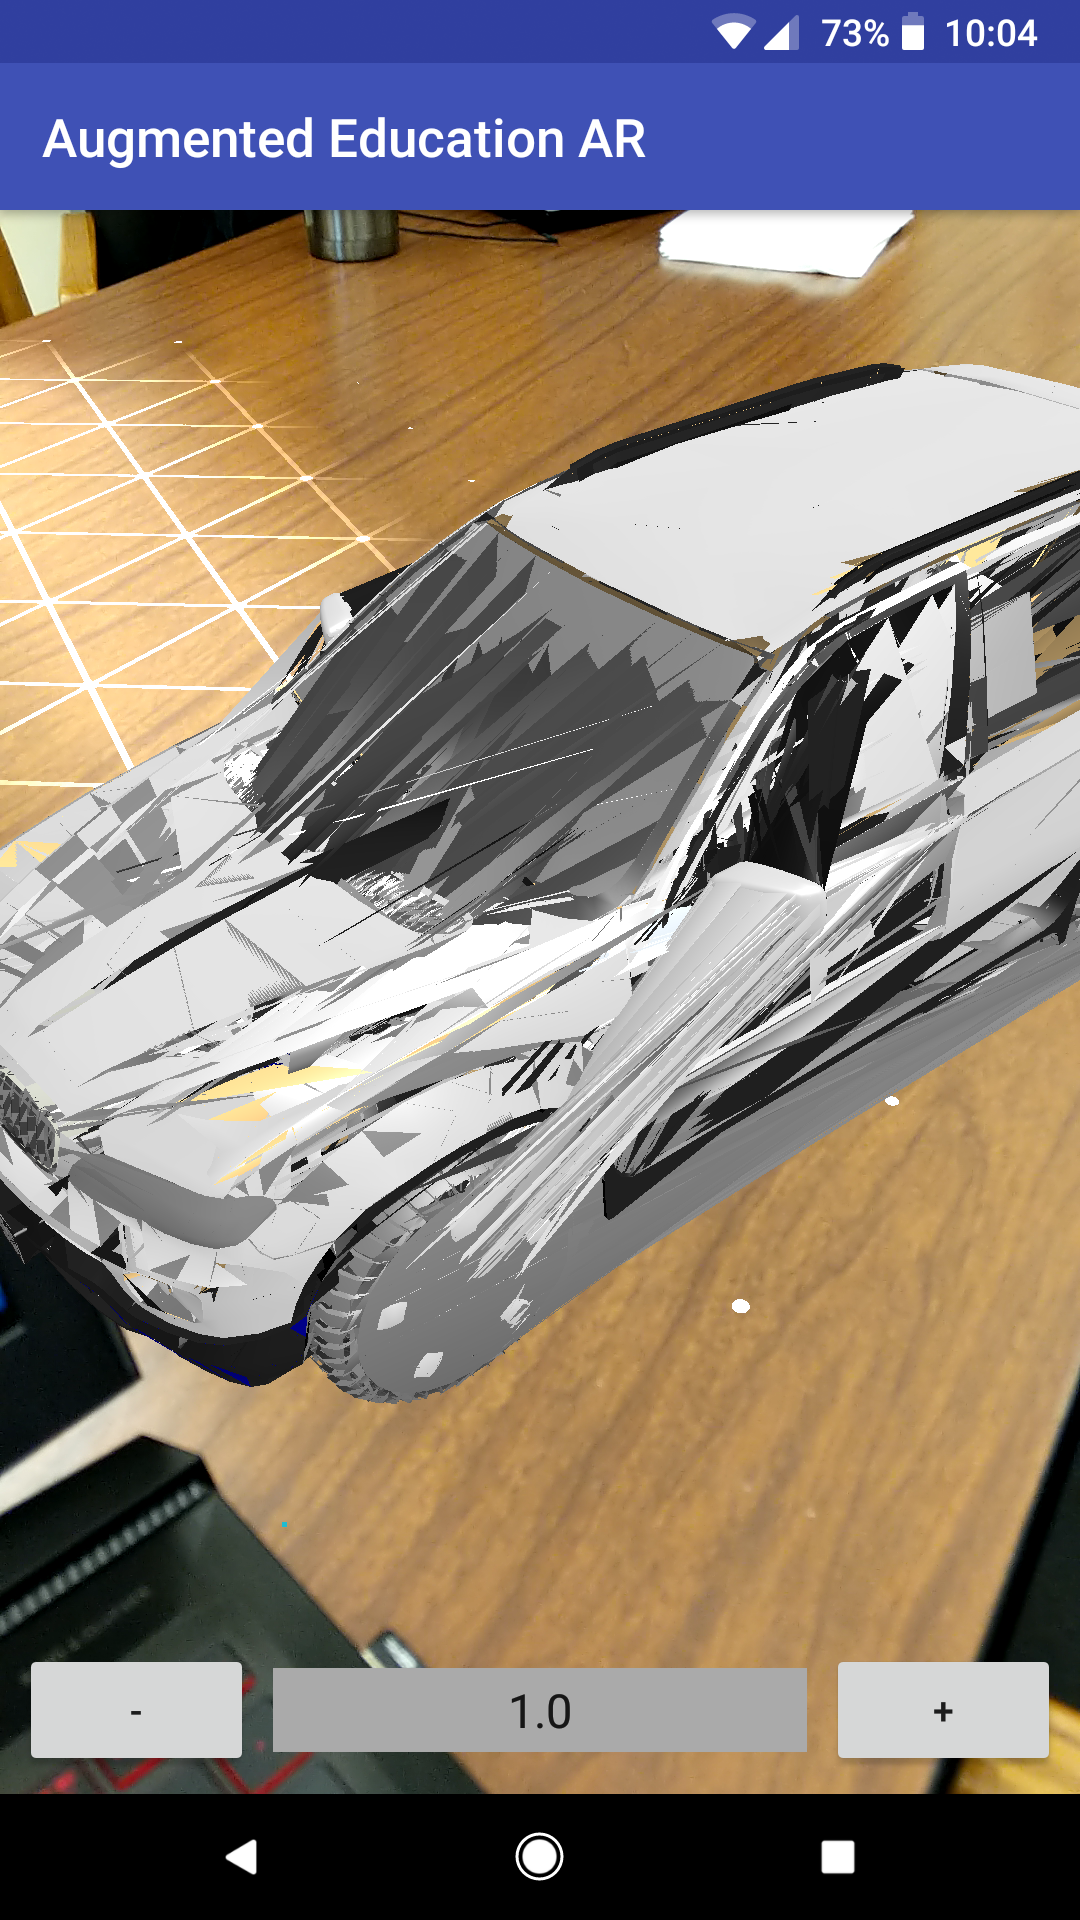
\includegraphics[width=0.5\textwidth]{Mobile/Mobile_BMW}
                \centering
                \caption{Large File - BMW}
                \label{fig:mobileBMW}
            \end{figure}
    
        \subsubsection{Small Files}
            A simple test used especially at the beginning of development to test that models would draw. The sphere is a typical example of something generated from Maple. 
        
            \begin{figure}[H]
                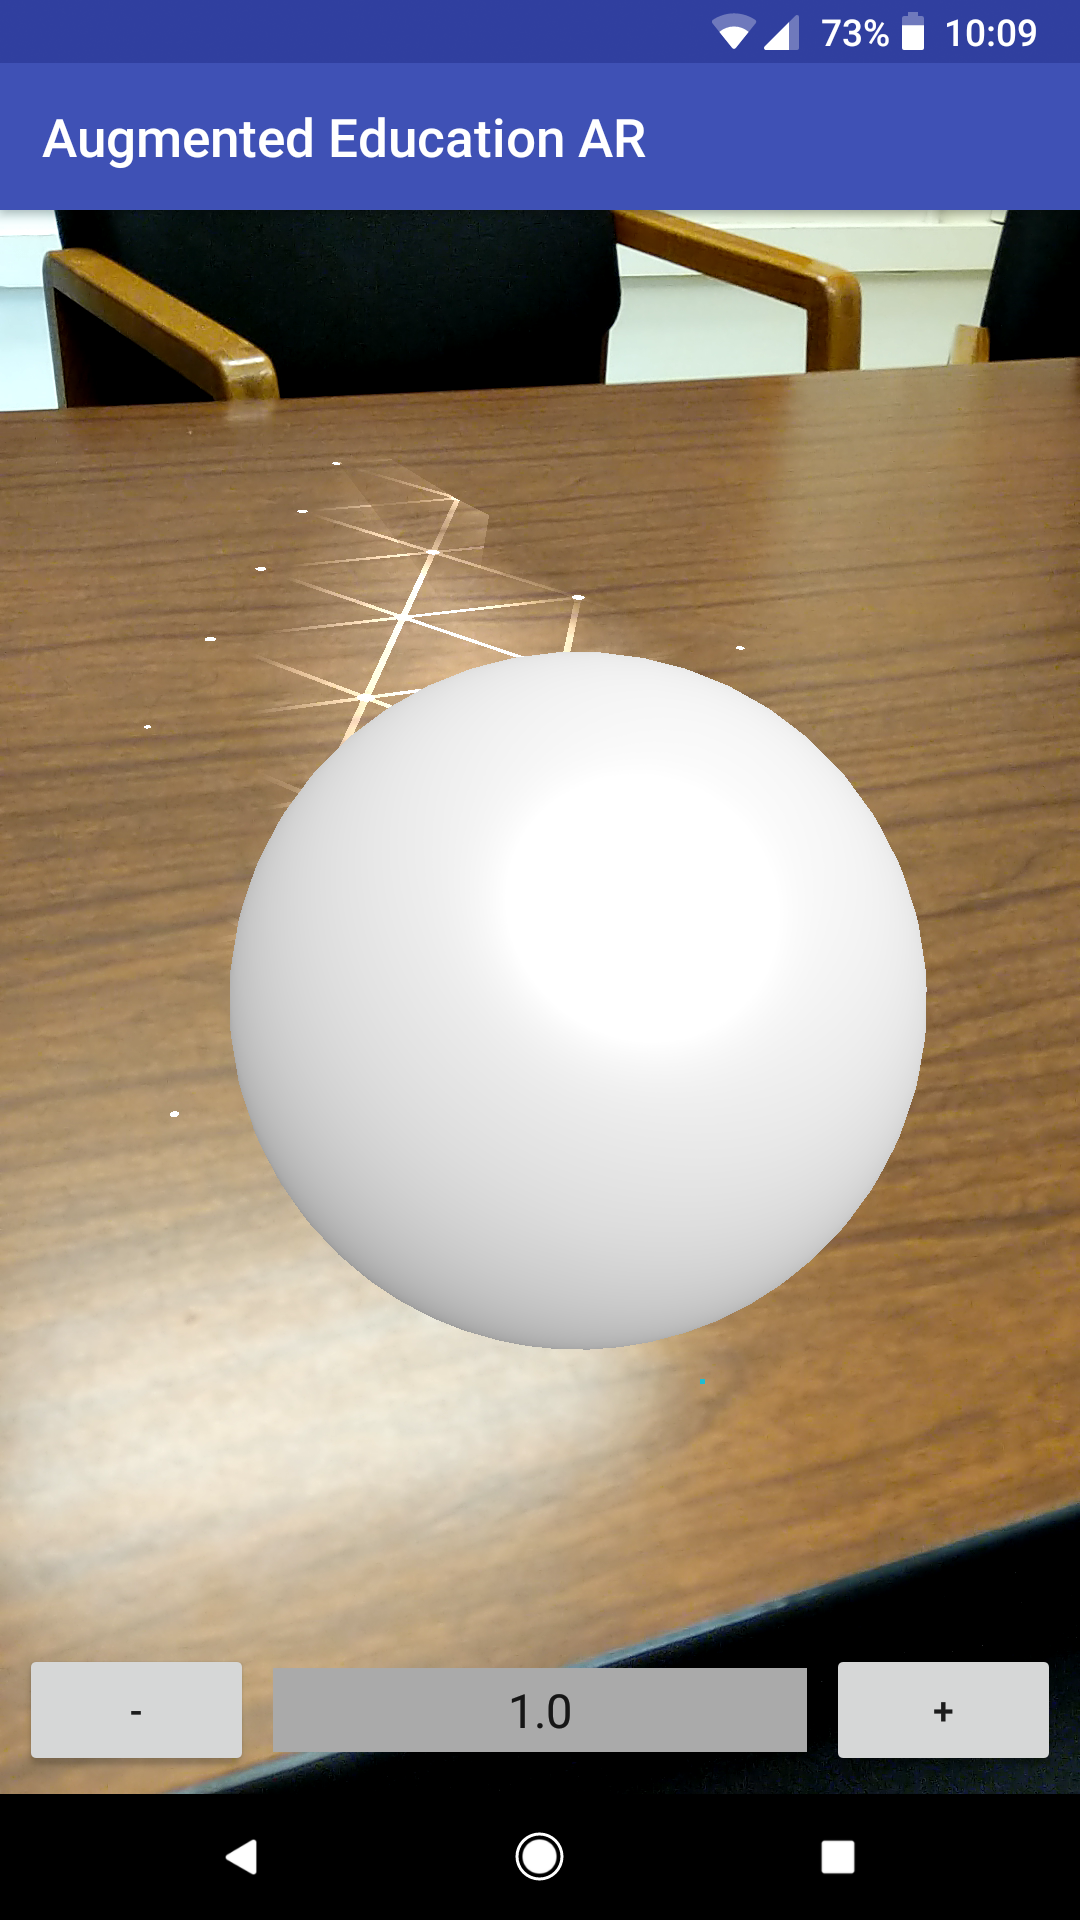
\includegraphics[width=0.5\textwidth]{Mobile/Mobile_Sphere}
                \centering
                \caption{Small File - Sphere}
                \label{fig:mobileSphere}
            \end{figure}
            
        \subsubsection{Embedded Images}
            
            Some 3D modeling software generates OBJ files with PNG textures referenced in the MTL instead of defining RGB values. It was necessary to test that these files were also supported by the app after adding extra functionality for them. Figure \ref{fig:mobileEmbeddedPhone} shows the PNG texture working, but it doesn't match the intended plot perfectly (Figure \ref{fig:mobileEmbeddedWindows}). This is because the app currently does not support drawing multiple images on top of each other yet.
        
            \begin{figure}[H]
                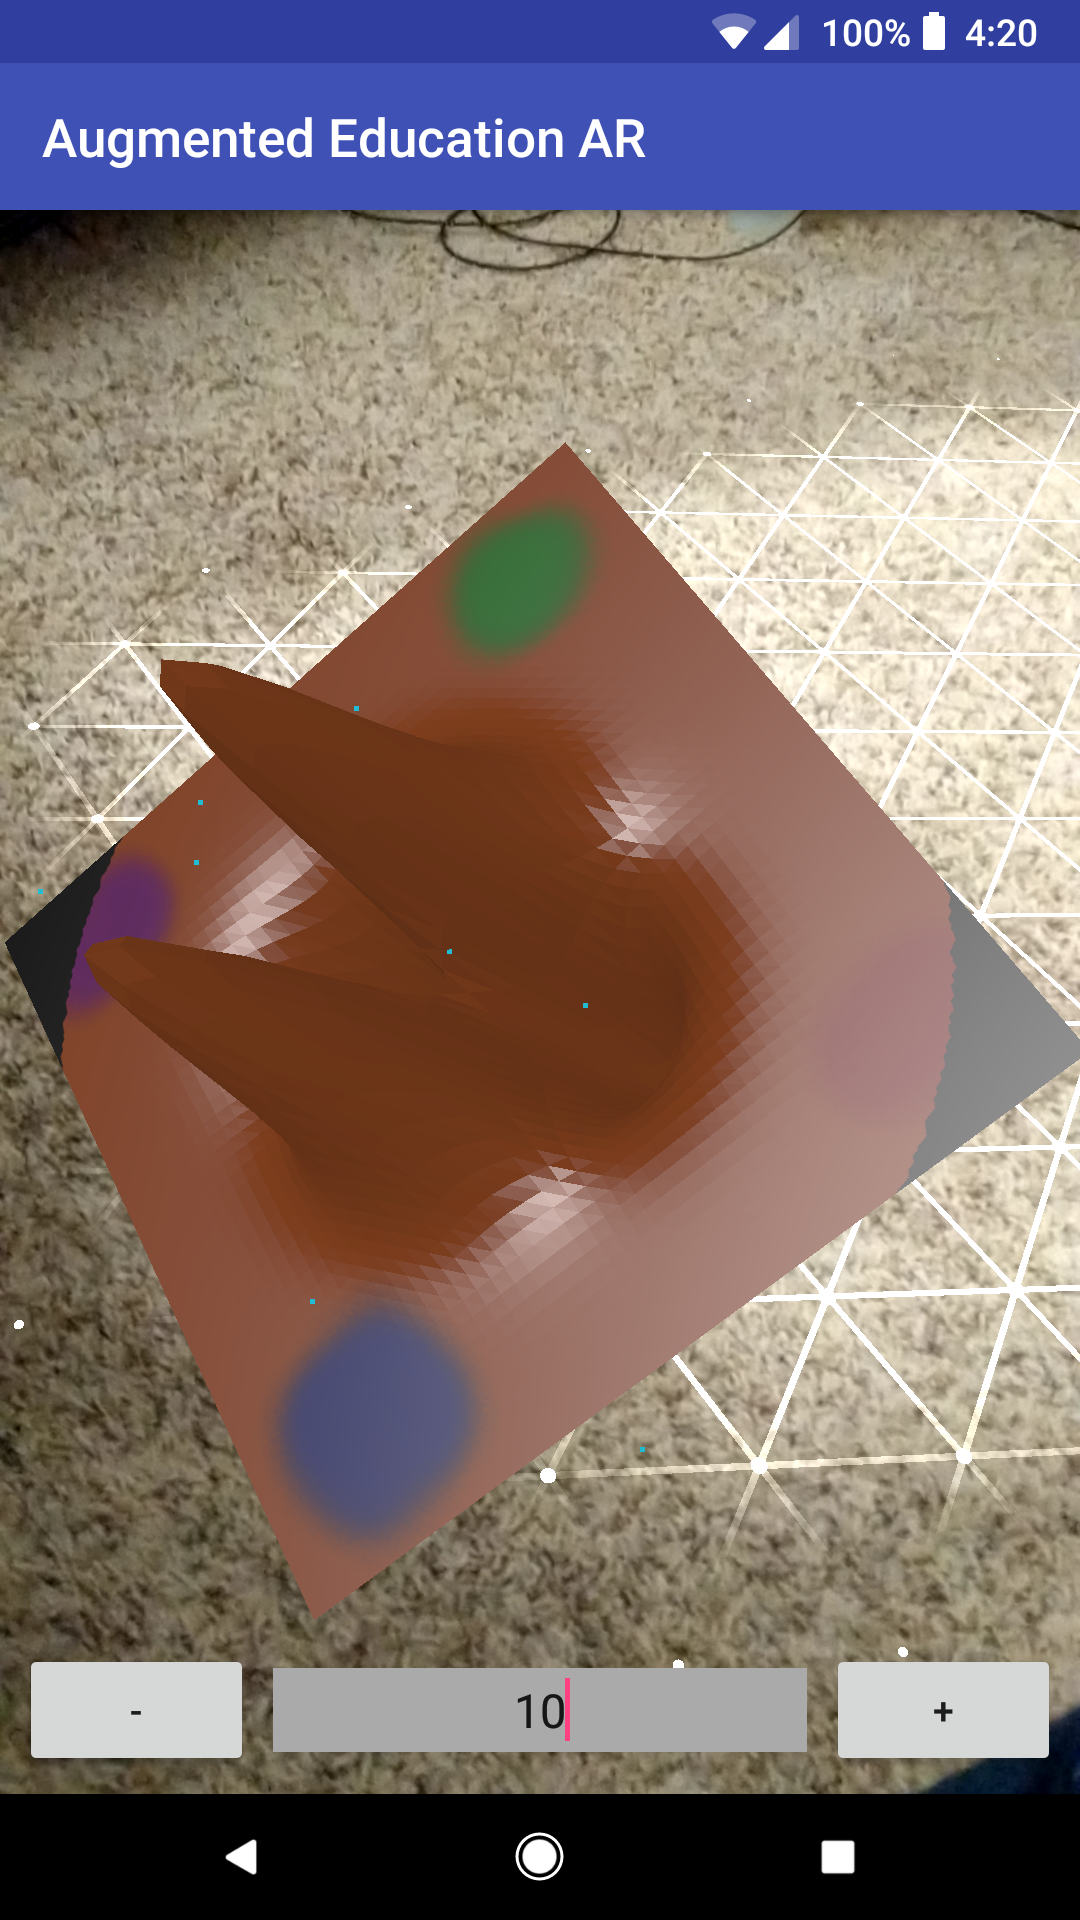
\includegraphics[width=0.5\textwidth]{Mobile/Mobile_ImagesPhone}
                \centering
                \caption{Embedded Image - Viewing on the phone}
                \label{fig:mobileEmbeddedPhone}
            \end{figure}

            \begin{figure}[H]
                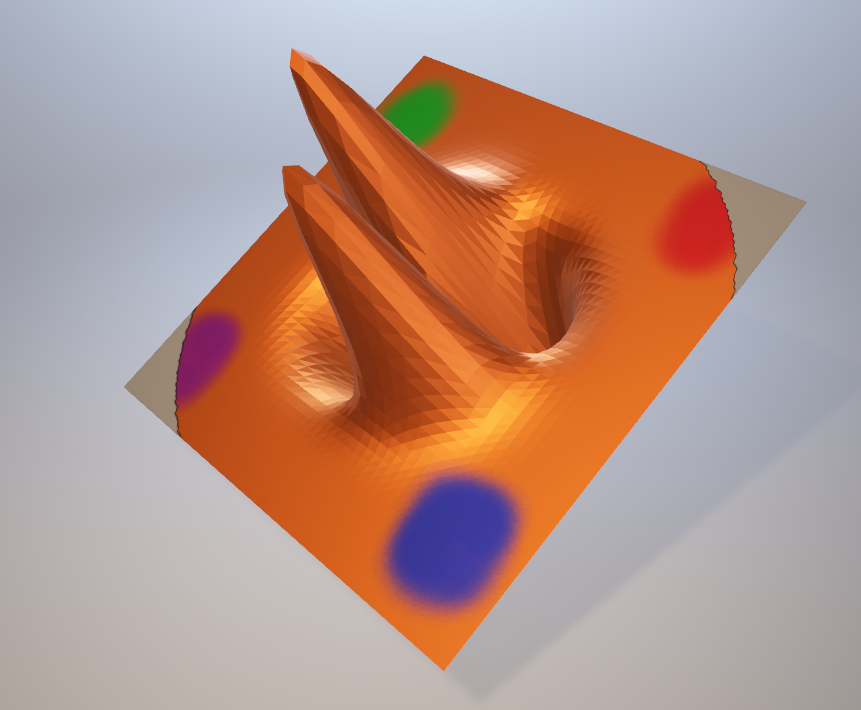
\includegraphics[width=0.5\textwidth]{Mobile/Mobile_ImagesWin}
                \centering
                \caption{Embedded Image - Viewing in the Windows Viewer}
                \label{fig:mobileEmbeddedWindows}
            \end{figure}

        \subsubsection{Scaling}

            Different models scale differently when initially drawn in the app. A scale factor of 1.0 on one model may be too small or too large, making the model difficult to visualize. To remedy this, the app provides an option to increase or decrease the scale factor, as well as change the step so models of different scales can be adjusted properly. Maple models generally need a larger scale factor (approx 3.0) while others like the car need to be adjusted by 0.1 at a time.
        
    \subsection{Web Interface}

        Another major component of the mobile app was the communication with the website.  If the app can display the models, there is little purpose if there is no method to get the models onto the phone.  The web API provided by the web team provides a method for communicating with the website.  It is done using the Volley library, provided by Google.  It abstracts the low level sending/receiving of networking communication away from the developer.  The code for these interfaces in primarily located in the \texttt{WebAccessor} Java class.

        Testing has shown that while the website is on Azure, the responsiveness is not always the best.  It is not infrequent to receive timeout errors on requests.  When this occurs, a message is displayed to the user.
        
        \subsubsection{Endpoints}\label{sec:Mobile_Auth}
        
            The endpoints used by the mobile application allow the app to: authenticate with the website, get a list of owned models, and download a model.  The endpoints were tested using Postman (to make sure the response was what was expected), the Android Studio debugger to make sure the correct fields were set, and a packet capture application to view the actual HTTP message sent from the phone.

            \paragraph{Authenticate}

                The authentication endpoint allowed the user to provide a username and password to get access to the website.  If the user entered valid credentials, an auth token is returned that allows the application to make requests on behalf of the user.  The auth token is used in the other API calls to the server.

                This API call is only performed on the Main Activity screen (the login page).  If a user is not authenticated, the user cannot continue through the app unless they select the Offline Mode button to not perform future web communication tasks.  A success of this component was, if the user supplied valid credentials, a valid auth token was returned.  Otherwise, an error message should be printed.  The testing was performed manually by trying invalid usernames/passwords.  In these cases, the website did not provide a valid auth token.  When correct usernames/passwords were entered, an auth token is returned.

                The Postman view that was used to test the endpoint (on the web side) is shown in Figure \ref{fig:mobilePostmanGetAuthToken}.

                \begin{figure}[H]
                    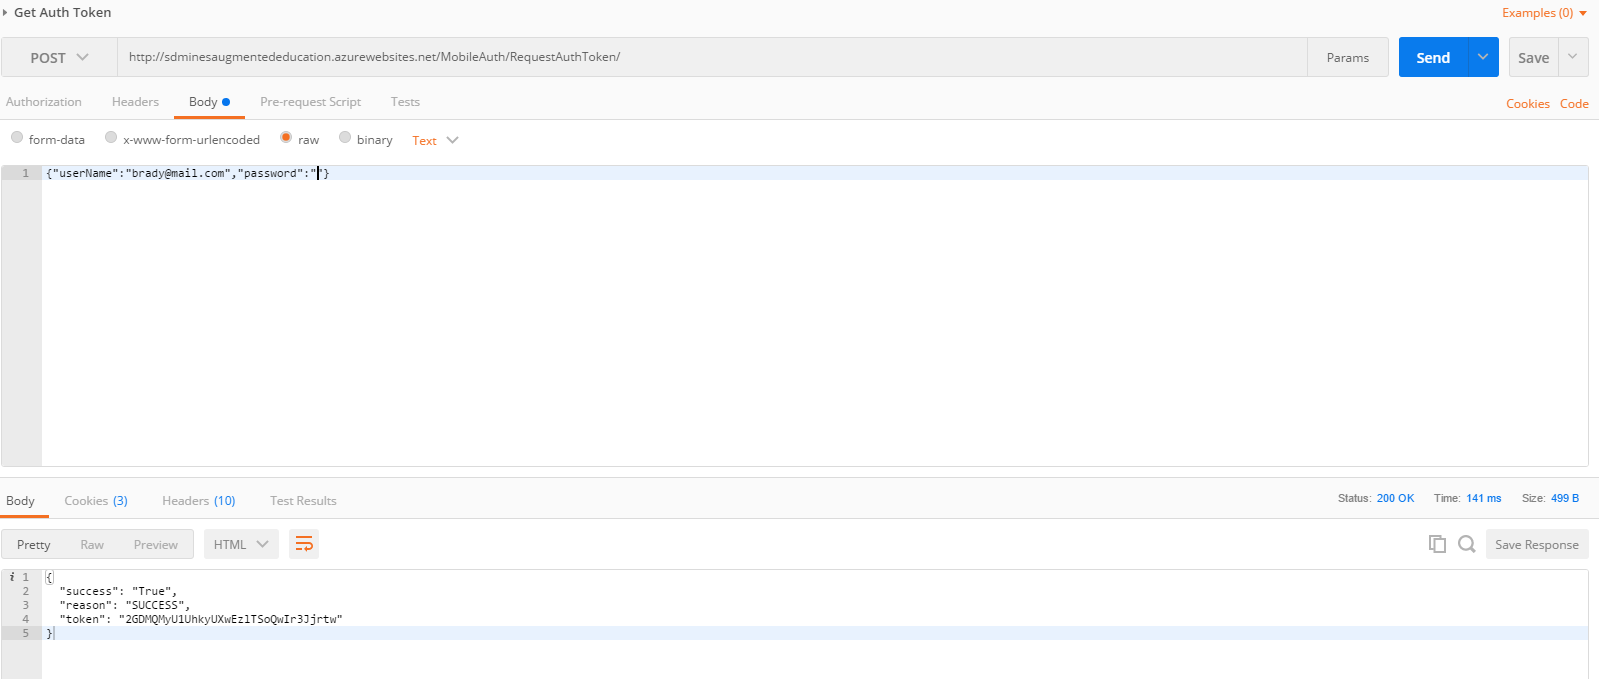
\includegraphics[width=0.75\textwidth]{postman_GetAuthToken}
                    \centering
                    \caption{Postman - Get authentication token}
                    \label{fig:mobilePostmanGetAuthToken}
                \end{figure}
                
            \paragraph{List Models}

                Another endpoint that is used by the mobile device is the one to get a listing of files owned by the user.  Like with the authentication token request, this call was tested manually to ensure the HTTP packets were well formed, and as expected.  Postman was again used to help test.  Figure \ref{fig:mobilePostmanListFiles} shows the Postman setup to send a request for a file listing.  
                
                \begin{figure}[H]
                    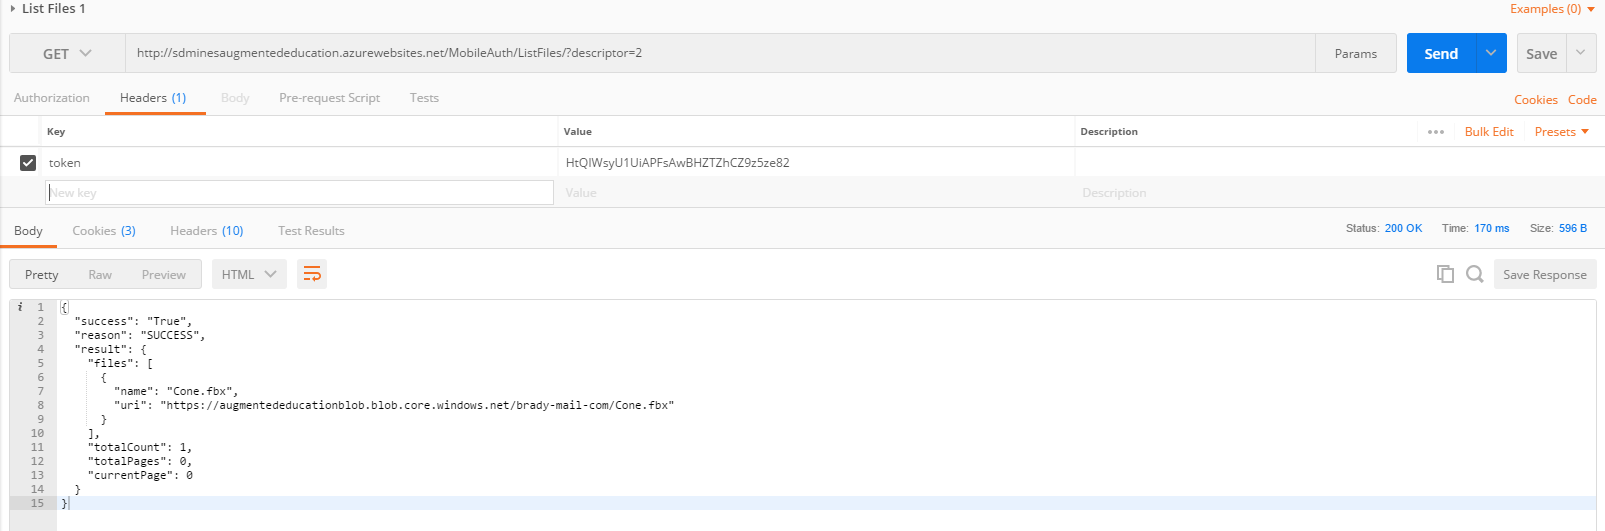
\includegraphics[width=0.75\textwidth]{postman_ListFiles}
                    \centering
                    \caption{Postman - List files}
                    \label{fig:mobilePostmanListFiles}
                \end{figure}
                
                Note, the \texttt{descriptor=} at the end of the URL, as it is used to state which files are desired for download.  An agreement was made between the mobile and web teams on what the levels should be.  There is an enumeration defined in the Java code with more details on the values and meanings.  Testing the different values showed a bug in the web code that always caused an error on the mobile device.  This issue was fixed by the web team.
            
            \paragraph{Download Model}

                Downloading a model includes contacting two endpoints.  One is used to get a temporary link to actually download the file, and the next downloads the file from that URL.  This is used so the phone can store the long term location, and get a temporary active URL to get the file.  Testing for these sections again included using Postman, and using a web browser to facilitate the download.  The Postman settings to get the temporary URL are located in Figure \ref{fig:mobilePostmanDownloadFile}.

                \begin{figure}[H]
                    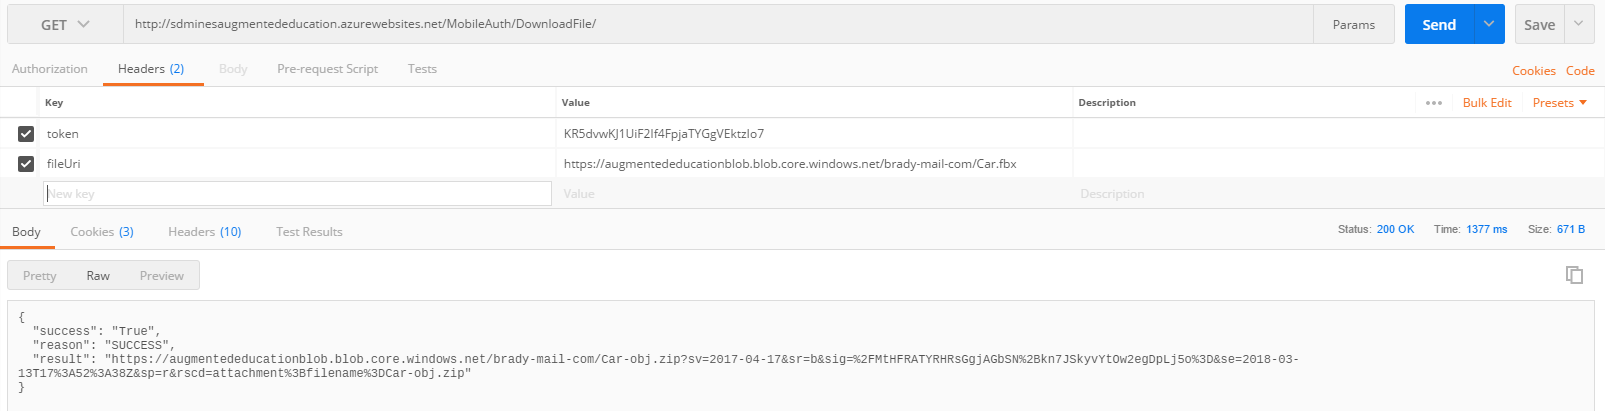
\includegraphics[width=0.75\textwidth]{postman_DownloadFile}
                    \centering
                    \caption{Postman - Download a file}
                    \label{fig:mobilePostmanDownloadFile}
                \end{figure}

                The field \texttt{result} contains the temporary URL.  It would then be put into a web browser (typically Firefox or Chrome) and the file is downloaded.  The file downloaded should be in the OBJ file format, since it is the one that is parse-able by the phone.  The website should use the file conversion software ensure this.  When the models are downloaded, they are stored in a \texttt{Models} directory on the phone.  The file system on the device can be viewed with the Downloads app.  Note, if the model is downloaded, and it does not show up in the file structure, the phone should be restarted.  Commonly, the files do not show up until the device is restarted.  A new folder will be created in the \texttt{Models} directory.  This is because one OBJ model can have multiple other models associated with it, including MTL (material) files and images.  When the models are downloaded, a zip archive is actually downloaded and extracted.

                Future developers should be aware of how the models are saved from the Android download manager.  When making the call for the download manager to do the download, a final path/file name must be provided.  This can cause issues if the file is saved with the wrong extension, especially if the files are viewed on the developers computer (and not just on the phone).
        
        \subsubsection{No Internet}

            Since internet can be less than reliable on cell phones, it was important to test if the there was no internet on the phone.  This was done by turning off Wifi on the testing phones (as they do not have cellular activated).  As expected, if there is no internet, an error message is displayed to the user that the communication was unsuccessful.
        
    \subsection{Offline Mode}
        
        When preparing for the Senior Design Fair, the mobile team decided that it would be a good idea to add an offline mode so the user can view models without having to authenticate with the server.  This was because the Wifi capabilities at the fair would be slim to none.  Therefore, an "Offline Mode" button was added to the login page to allow the user to continue offline.  Testing needed to be done on this to only show models registered as on the phone, as the user would not be able to download remote files without first authenticating.  This was tested and implemented in the application.  The application will not get a list of models from the website or download files from the website in offline mode.  The rest of the functionality (such as viewing the models) remained the same, which was as desired.

    \subsection{QR Code Scanning}
        
        To test that the app was scanning QR codes as expected during development, the team tried a number of different QR codes found online and printed on objects around. There were a surprising amount of these objects on hand with printed QR codes to test with. Testing on these gave an idea of the performance of the QR code scanner for varying QR code sizes.

        The scanner worked with QR codes that pointed to the 3D model downloads.  One difficulty of testing this was the way that the list of models was populated.  When the list was originally populated, all models owned by the user, and models that were public were added to the list.  So, all of the models that the user could access would already be in the list, so scanning a QR code would do nothing.  A later revision changed this so only privately owned files were added to the list, so QR codes can now usefully be scanned. Once the team had the functionality to embed the download link in a QR code, the team tested downloading a number of files manually using their respective QR codes.

    \subsection{Database}
        
        To test the database, the team primarily tested manually by using the test 3D model files. The database is populated by all the models private to the user's account. The team verified that when models are added to the user's account, the database is updated with a listing of the new models. The database also adds entries for scanned QR code files.

%This chapter describes the results and conclusions of your research.   This would be the final report for a research project.  
%
%\section{Result 1}
%
%\section{Result 2}
%
%\section{Conclusions}
%
%\section{Further work}    %% Research track  only

\bibliographystyle{plain}
\bibliography{designrefs.bib}
\addcontentsline{toc}{chapter}{Bibliography}


% We want to add the Software agreement to the end and number the
% pages separately from the document.  We don't want to do a standard
% chapter heading, but we do want it to appear in the table of contents
% and in the index used for on-line viewing.  We defined the \agreement
% macro to set things up for us.
\agreement

\chapter{Software Agreement}
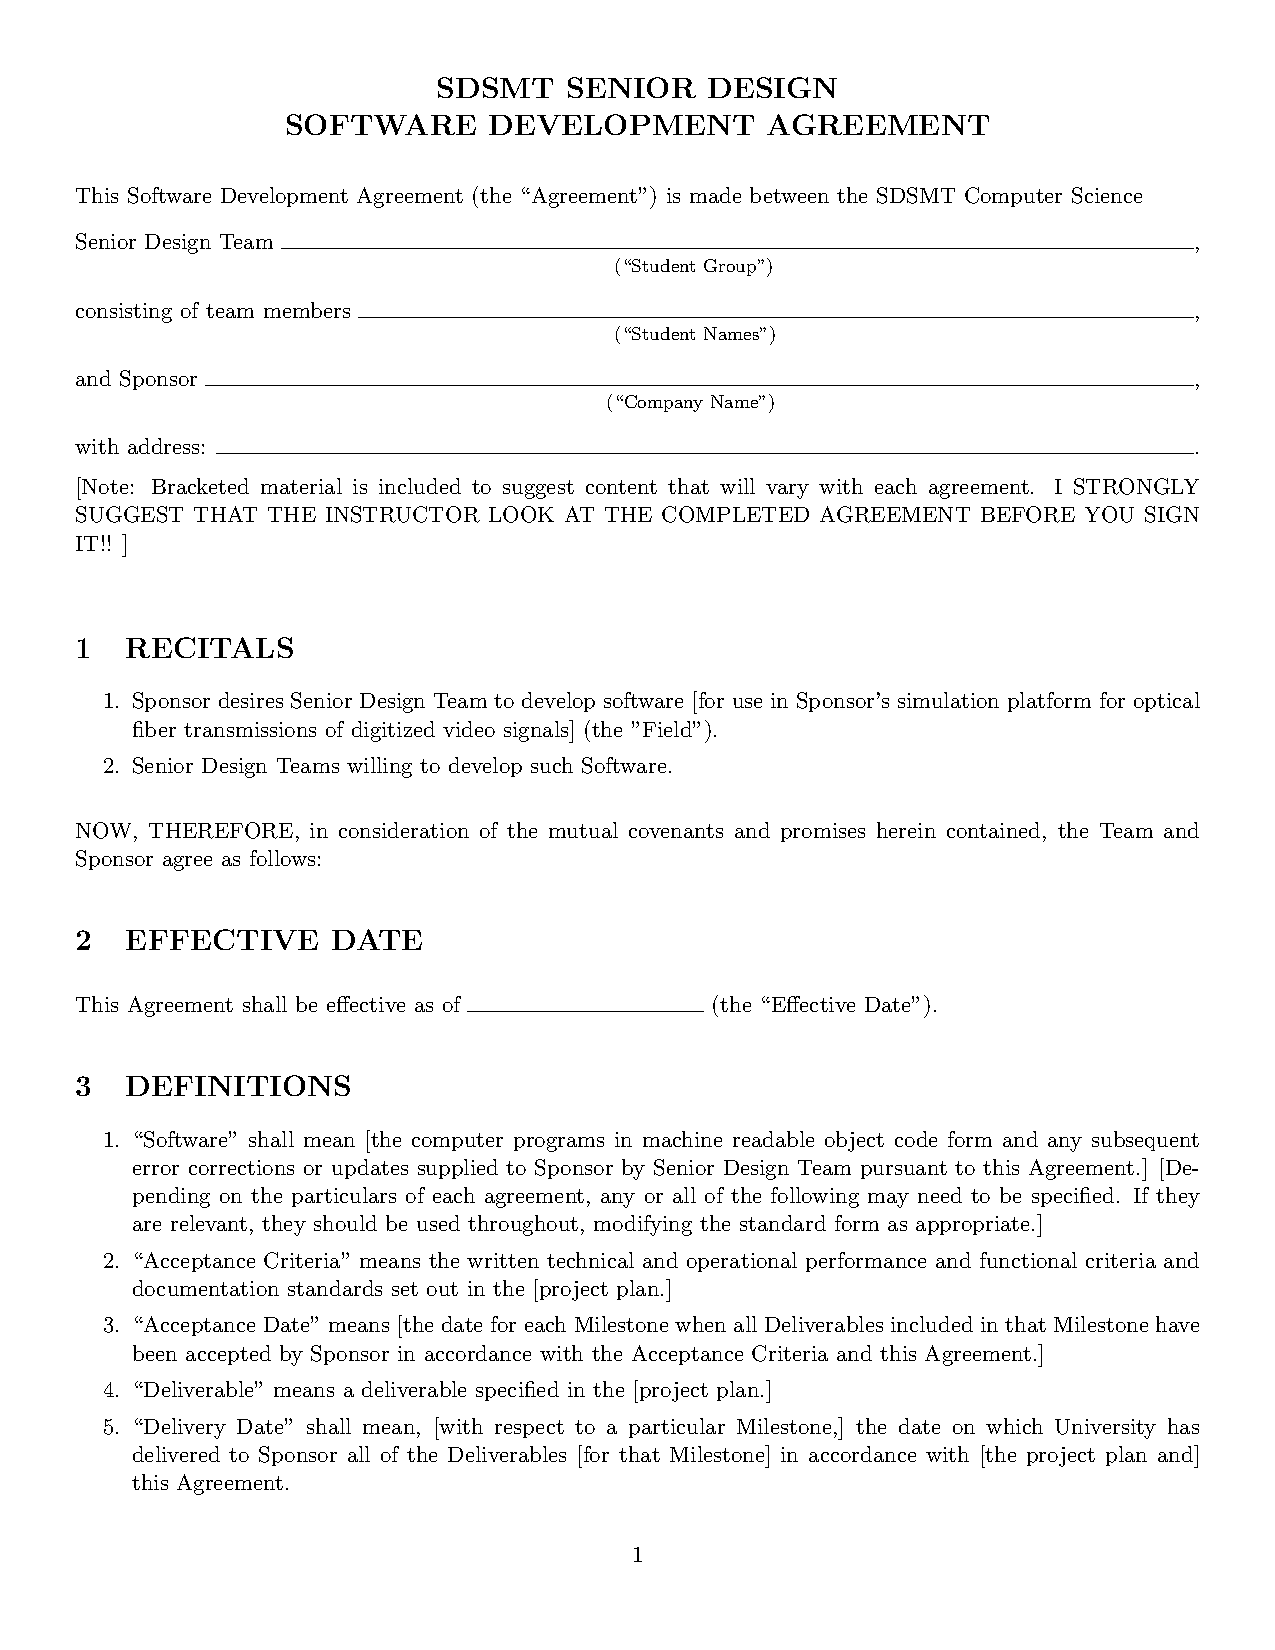
\includepdf[pages={1-4}]{SoftwareContract.pdf}

% In our style file, appendices are numbered with capital letters
\appendix

\chapter{Product Description}
The final product will include the following features:

\begin{enumerate}
	\item Web Team:
	\begin{itemize}
		\item Password protected user login page. 
		\item Ability to upload supported 3D CAD files. 
		\item Uploaded files will be stored in cloud.
		\item Upon request, a unique direct download link and QR code associated with the file will be generated and supplied to user. 
		\item Uploaded files will be converted to the correct file type supported by the requesting AR device via Conversion Software.
		\item Upon accessing download link or QR code, associated file with appropriate type will be delivered to supported device.
		\item Users will be able to manage permissions of their files to make them private or public.
		\item Users may update files to replace the existing file.
		\item Users may delete files. 
		\item Converted files (not originals) that remain unused for period of time may be deleted by the website to avoid wasting cloud storage space.  
	\end{itemize}
	\item Conversion Software:
	\begin{itemize}
		\item Will convert supported input file type to specified and supported output file type. 
		\item Will be written in C++. 
		\item Will be hosted on back end of website. 
		\item Will support the following input file types: FBX, DAE, BLEND, OBJ, STL, PLY.
		\item Will support the following output file types: FBX, DAE, OBJ, STL, PLY.
	\end{itemize} 
\end{enumerate}

Milestones:

\begin{itemize}
	\item 9/18/2017    - Define milestones and user stories
	
	\item 10/2/2017    - Base website created with file upload ability
	
	\item 10/16/2017  - Wire frames, Presentation 1 documents, standalone file conversion
	
	\item 10/30/2017  - File upload/download, file conversion integrated
	
	\item 11/13/2017  - QR code generation, standalone advanced file conversion 
	
	\item 11/27/2017  - File conversion integration, create users, Presentation 2 documents
	
	\item 12/04/2017   - Finish documentation, second semester prep
	
	\item 12/13/2017  - MVP delivered to sponsor

	\item 04/27/2017  - Final product delivered to sponsor.
\end{itemize}


\vspace{2\baselineskip}
\centerline{\Large {\bf NOTE:} {\em Appendix A is part of the contract.}}




% !TEX root = DesignDocument.tex


\chapter{Class Index}
% !TEX encoding = UTF-8 Unicode
% !TEX root = DesignDocument.tex

\section{Website}

\section{File Conversion}

\begin{DoxyCompactList}

    
\item \contentsline{section}
{\hyperlink{website_component1}{Component 1} }
{\pageref{website_component1}}{}
    
\item \contentsline{section}
{\hyperlink{fileconversion_parseparameters}{ParseParameters} }
{\pageref{fileconversion_parseparameters}}{}

\item \contentsline{section}
{\hyperlink{fileconversion_abstractconverter}{AbstractConverter} }
{\pageref{fileconversion_abstractconverter}}{}

\item \contentsline{section}
{\hyperlink{fileconversion_assimpconverter}{AssimpConverter} }
{\pageref{fileconversion_assimpconverter}}{}

\end{DoxyCompactList}

\chapter{Class Documentation}
\hypertarget{class_poly}{\section{Poly Class Reference}
\label{class_poly}\index{Poly@{Poly}}
}
\subsection*{Public Member Functions}
\begin{DoxyCompactItemize}
\item 
\hyperlink{class_poly_aa3def076b74bed67904976ad4f9fe9b1}{Poly} ()
\item 
\hyperlink{class_poly_a2f8530284140c31c0aa391dd4d0b61be}{$\sim$\-Poly} ()
\item 
int \hyperlink{class_poly_a14a7ad77ce612b0c54f531d307ee4b39}{myfunction} (int)
\end{DoxyCompactItemize}


\subsection{Constructor \& Destructor Documentation}
\hypertarget{class_poly_aa3def076b74bed67904976ad4f9fe9b1}{\index{Poly@{Poly}!Poly@{Poly}}
\index{Poly@{Poly}!Poly@{Poly}}
\subsubsection[{Poly}]{\setlength{\rightskip}{0pt plus 5cm}Poly\-::\-Poly (
\begin{DoxyParamCaption}
{}
\end{DoxyParamCaption}
)}}\label{class_poly_aa3def076b74bed67904976ad4f9fe9b1}
My constructor \hypertarget{class_poly_a2f8530284140c31c0aa391dd4d0b61be}{\index{Poly@{Poly}!$\sim$\-Poly@{$\sim$\-Poly}}
\index{$\sim$\-Poly@{$\sim$\-Poly}!Poly@{Poly}}
\subsubsection[{$\sim$\-Poly}]{\setlength{\rightskip}{0pt plus 5cm}Poly\-::$\sim$\-Poly (
\begin{DoxyParamCaption}
{}
\end{DoxyParamCaption}
)}}\label{class_poly_a2f8530284140c31c0aa391dd4d0b61be}
My destructor 

\subsection{Member Function Documentation}
\hypertarget{class_poly_a14a7ad77ce612b0c54f531d307ee4b39}{\index{Poly@{Poly}!myfunction@{myfunction}}
\index{myfunction@{myfunction}!Poly@{Poly}}
\subsubsection[{myfunction}]{\setlength{\rightskip}{0pt plus 5cm}int Poly\-::myfunction (
\begin{DoxyParamCaption}
\item[{int}]{a}
\end{DoxyParamCaption}
)}}\label{class_poly_a14a7ad77ce612b0c54f531d307ee4b39}
my own example function fancy new function

new variable 

The documentation for this class was generated from the following file\-:\begin{DoxyCompactItemize}
\item 
hello.\-cpp\end{DoxyCompactItemize}

  %% All tracks


% !TEX encoding = UTF-8 Unicode
% !TEX root = DesignDocument.tex

\chapter{Business Plan}
\includepdf[pages={1-33}]{InTouchLLCBusinessPlan.pdf}

   %% Entrepreneur track only 
% !TEX root = DesignDocument.tex


\chapter{Experimental Log}

For research projects one needs to keep a log of all research/lab activities.   

%% If you have multiple labs, you may want to break the labs into sections, check 
%% with the profession on format.
%% \section{Lab 1}

\begin{description}
\item [10/15/15]  Ran modified filter on data sets 1 - 6.  Results were ...
\item [10/17/15]  Changed tolerance on sensor and collected data.  These ...
\end{description}   %% Research track  only


% \chapter{Publications}   %% Research track 
% % !TEX root = DesignDocument.tex


Research Track:  
This chapter will include any publications generated from the research.  Most likely these will be preprints and one will just include the pdf.

%\includepdf[pages={1-5}]{Pub1.pdf}



\chapter{Acknowledgment}
\label{SpecialThanks}  
Special thanks to Dr. Christer Karlsson, Dr. Jeff McGough, Dr. Adam Piper, Dr. Brent Deschamp, and Dr. King Adkins for your time spent ensuring this product will make an impact in the classroom. 
\vspace{\baselineskip}

Special thanks to Todd Gagne for your time spent mentoring development of the InTouch L.L.C. business plan. 


\chapter{Supporting Materials}
\label{ch:support}

These are materials that we refer to in our documentation. It includes the 
mobile computing grant submitted by Dr. McGough and other professors from 
various departments at SD Mines.


\section{Mobile Computing Grant}
\includepdf[pages={1-8}]{MobileComputingGrant2017.pdf}

\section{HoloLens Bridge Demo at Intersection of SD Mines and Main St, Rapid City, SD}


\section{HoloLens Classroom Bridge Demo}

\section{Mobile App Sine Wave Demo}


\section{Mobile App Sphere Demo}


\section{Mobile App Car Demo}


\section{ARCore Demo}


\section{Senior Design Poster}
\includepdf{AE_Senior_Design_Poster.pdf}

\section{Senior Design Fair Media Handout}
\includepdf[pages={1-1}]{SeniorDesignFairMediaHandout.pdf}

\section{Giant Vision Poster}
\includepdf[pages={1-1}]{GiantVisionPoster.pdf}

\section{Giant Vision Media Handout}
\includepdf[pages={1-1}]{GiantVisionMediaHandout.pdf} 

% chapters in backmatter don't have numbers, but they appear in the
% table of contents, and are numbered BM-X where X is the page number
% relative to where the backmatter begins.
\backmatter

%% Example
%\chapter{Course Syllabus}
%\includepdf[pages={1-17}]{syllabus.pdf}

%%% Remove after reading
%\chapter{\LaTeX\ Example}
%% !TEX root = DesignDocument.tex


\LaTeX\xspace sample file:  {\color{red} Remove from submitted materials}

\section{Introduction}
This is a sample input file.  Comparing it with the output it
generates can show you how to produce a simple document of
your own.

\section{Ordinary Text}  % Produces section heading.  Lower-level
                                    % sections are begun with similar 
                                    % \subsection and \subsubsection commands.

The ends  of words and sentences are marked 
  by   spaces. It  doesn't matter how many 
spaces    you type; one is as good as 100.  The
end of   a line counts as a space.

One   or more   blank lines denote the  end 
of  a paragraph.  

Since any number of consecutive spaces are treated like a single
one, the formatting of the input file makes no difference to
      \TeX,         % The \TeX command generates the TeX logo.
but it makes a difference to you.  
When you use
      \LaTeX,       % The \LaTeX command generates the LaTeX logo.
making your input file as easy to read as possible
will be a great help as you write your document and when you
change it.  This sample file shows how you can add comments to
your own input file.

Because printing is different from typewriting, there are a 
number of things that you have to do differently when preparing 
an input file than if you were just typing the document directly.  
Quotation marks like 
       ``this'' 
have to be handled specially, as do quotes within quotes: 
       ``\,`this'                  % \, separates the double and single quote.
        is what I just 
        wrote, not  `that'\,''.  

Dashes come in three sizes: an 
       intra-word 
dash, a medium dash for number ranges like 
       1--2, 
and a punctuation 
       dash---like 
this.

A sentence-ending space should be larger than the space between words
within a sentence.  You sometimes have to type special commands in
conjunction with punctuation characters to get this right, as in the
following sentence.
       Gnats, gnus, etc.\    % `\ ' makes an inter-word space.
       all begin with G\@.   % \@ marks end-of-sentence punctuation.
You should check the spaces after periods when reading your output to
make sure you haven't forgotten any special cases.
Generating an ellipsis 
       \ldots\    % `\ ' needed because TeX ignores spaces after 
                  % command names like \ldots made from \ + letters.
                  %
                  % Note how a `%' character causes TeX to ignore the 
                  % end of the input line, so these blank lines do not
                  % start a new paragraph.
with the right spacing around the periods 
requires a special  command.  

\TeX\ interprets some common characters as commands, so you must type
special commands to generate them.  These characters include the
following: 
       \$ \& \% \# \{ and \}.

In printing, text is emphasized by using an
       {\em italic\/}  % The \/ command produces the tiny extra space that
                       % should be added between a slanted and a following
                       % unslanted letter.
type style.  

\begin{em}
   A long segment of text can also be emphasized in this way.  Text within
   such a segment given additional emphasis 
          with\/ {\em Roman} 
   type.  Italic type loses its ability to emphasize and become simply
   distracting when used excessively.  
\end{em}

It is sometimes necessary to prevent \TeX\ from breaking a line where
it might otherwise do so.  This may be at a space, as between the
``Mr.'' and ``Jones'' in
       ``Mr.~Jones'',        % ~ produces an unbreakable interword space.
or within a word---especially when the word is a symbol like
       \mbox{\em itemnum\/} 
that makes little sense when hyphenated across 
       lines.

Footnotes\footnote{This is an example of a footnote.}
pose no problem.

\TeX\ is good at typesetting mathematical formulas like
       \( x-3y = 7 \) 
or
       \( a_{1} > x^{2n} / y^{2n} > x' \).
Remember that a letter like
       $x$        % $ ... $  and  \( ... \)  are equivalent
is a formula when it denotes a mathematical symbol, and should
be treated as one.

\section{Displayed Text}

Text is displayed by indenting it from the left margin.
Quotations are commonly displayed.  There are short quotations
\begin{quote}
   This is a short a quotation.  It consists of a 
   single paragraph of text.  There is no paragraph
   indentation.
\end{quote}
and longer ones.
\begin{quotation}
   This is a longer quotation.  It consists of two paragraphs
   of text.  The beginning of each paragraph is indicated
   by an extra indentation.

   This is the second paragraph of the quotation.  It is just
   as dull as the first paragraph.
\end{quotation}
Another frequently-displayed structure is a list.
The following is an example of an {\em itemized} list.
\begin{itemize}
   \item  This is the first item of an itemized list.  Each item 
          in the list is marked with a ``tick''.  The document
          style determines what kind of tick mark is used.

   \item  This is the second item of the list.  It contains another
          list nested inside it.  The inner list is an {\em enumerated}
          list.
          \begin{enumerate}
              \item This is the first item of an enumerated list that
                    is nested within the itemized list.

              \item This is the second item of the inner list.  \LaTeX\
                    allows you to nest lists deeper than you really should.
          \end{enumerate}
          This is the rest of the second item of the outer list.  It
          is no more interesting than any other part of the item.
   \item  This is the third item of the list.
\end{itemize}
You can even display poetry.
\begin{verse}
   There is an environment for verse \\    % The \\ command separates lines
   Whose features some poets will curse.   % within a stanza.

                           % One or more blank lines separate stanzas.

   For instead of making\\
   Them do {\em all\/} line breaking, \\
   It allows them to put too many words on a line when they'd 
   rather be forced to be terse.
\end{verse}

Mathematical formulas may also be displayed.  A displayed formula is
one-line long; multi-line formulas require special formatting
instructions.
   \[  x' + y^{2} = z_{i}^{2}\]
Don't start a paragraph with a displayed equation, nor make
one a paragraph by itself.

\section{Build process}

To build \LaTeX\ documents you need the latex program.  It is free and available on all operating systems.   Download and install.  Many of us use the TexLive distribution and are very happy with it.    You can use a editor and command line or use an IDE.  To build this document via command line:

\begin{verbatim}
alta>  pdflatex SystemTemplate
\end{verbatim}
If you change the bib entries, then you need to update the bib files:
\begin{verbatim}
alta>  pdflatex SystemTemplate
alta>  bibtex SystemTemplate
alta>  pdflatex SystemTemplate
alta>  pdflatex SystemTemplate
\end{verbatim}

The template files provided also contain a Makefile, which will
make things much easier.  

\section*{Acknowledgment}
Thanks to Leslie Lamport.  






\end{document}
